
\newcommand{\fCII} {\emath{f^{C \times 2}}}
\newcommand{\fPII} {\emath{f^{P \times 2}}}
\section{Experimental Results on Synthetic Data}\label{sec:synData}
\label{section:results}

\subsection{Synthetic Scalar and Gradient Data}
\label{section:synthetic}

To measure the quality of our reconstruction,
we used a number of synthetic scalar and gradient data sets.
Given a point $p$,
let $f^{L_1}_{p}(q)$ be the $L_1$ distance from $p$ to $q$.
A Cube data set is generated by sampling $f^{L_1}_p$
and its gradients on vertices of the regular grid.

Level sets of $f^{L_1}_p$ are cubes whose edges are
parallel to the coordinate axes
and whose facets are orthogonal to those axes.
By rotating $f^{L_1}_p$ around $p$, 
we can generate a scalar field whose level sets are cubes
that are not axis-aligned.
By taking the minimum of two (rotated) scalar fields, 
$f^{L_1}_p$ and $f^{L_1}_{p'}$, 
centered around two different points, $p$ and $p$', respectively,
we get a scalar field whose level sets are the boundaries
of the unions of the two cubes.
We call such data sets TwoCubes and use them 
with various rotations as test sets.

Let $\ell$ be a line.
Let $f^C_{\ell}(q)$ be the Euclidean distance from point $q$ to $\ell$.
The level sets of $f^C_{\ell}(q)$ are infinite cylinders around $\ell$.
Let $\fCII_{\ell,r}(q)$ equal $|f^C_{\ell}(q) - r|$.
The level sets of $\fCII_{\ell,r}(q)$  are pairs of infinite cylinders
at equal distances from the cylinder of radius $r$ around $\ell$.
Let $\fPII_{p,\ell}(q)$ be the distance from $q$ to the plane 
that contains point $p$ and is orthogonal to $\ell$.
Let $f^A_{p,\ell,r}(q)$ be the maximum 
of $\fCII_{\ell,r}(q)$ and of $\fPII_{p,\ell}(q)$.
The level sets are the boundaries of thickened annuli.

The width of the thickened annuli defined by $f^A_{p,\ell,r}$
equals their height.
We can adjust change the difference between the width and height
by adding a constant $c$ to $\fCII_{\ell,r}$.
Let $f^A_{p,\ell,r,c}(q)$ be the maximum 
of $\fCII_{\ell,r}(q)+c$ and of $\fPII_{p,\ell}(q)$.
If $c$ is positive, then the height is $c$ units greater than the width.
If $c$ is negative, then the height is $c$ units less than the width.

Define $f^F_{p,\ell,r,c}(q)$ as the minimum
of $f^A_{p,\ell,r,c}(q)$ and $f^A_{p,\ell,r,-c}(q)$.
The level sets of $f^F_{p,\ell,r,c}(q)$ are the boundaries
of the unions of two thickened annuli.
One annuli has height $c$ units greater than its width
while the other has height $c$ units less than its width.
A Flange data set is a regular grid sampling of $f^F_{p,\ell,r,c}(q)$. 
We use the Flange data sets as test sets.

\subsection{Isosurface Reconstruction on Synthetic Data}
We ran SHREC on 40 Flange datasets with different unique orientations. Figure~\ref{fig:flangeAngle} shows the summary results.
Figure~\protect\subref*{fig:flangeAngle3} shows the countDegree errors for SHREC with synthetic gradients and with RELIGRAD gradients computed directly from scalar data. With synthetic gradients, SHREC produced ``NO" degree errors on the 40 test cases.
With gradients computed from the scalar volume using RELIGRAD 32 cases (80$\%$) produced ``no" degree errors. The maximum number of error was 8.
Figure~\protect\subref*{fig:flangeAngle1} shows the number of simplices with angle difference greater than 30$^\circ$, 40$^\circ$ and 50$^\circ$ from the original mesh for the 40 test cases. Figure~\protect\subref*{fig:flangeAngle2} shows  the number of simplices versus the angle difference for one particular dataset (id 17). This particular dataset has no CountDegree errors, it has three simplices with surface angle difference equals or greater than 30 degrees from the original and one simplex above 40 degrees. The mesh itself has approximately 133 thousand simplices. 
Figure~\ref{fig:flange1} shows the result on a single dataset. The magnified region shows edges with dihedral angle less than $140^\circ$ in red blended with a subset of the ``non-sharp" edges. 
\begin{figure}[htb]
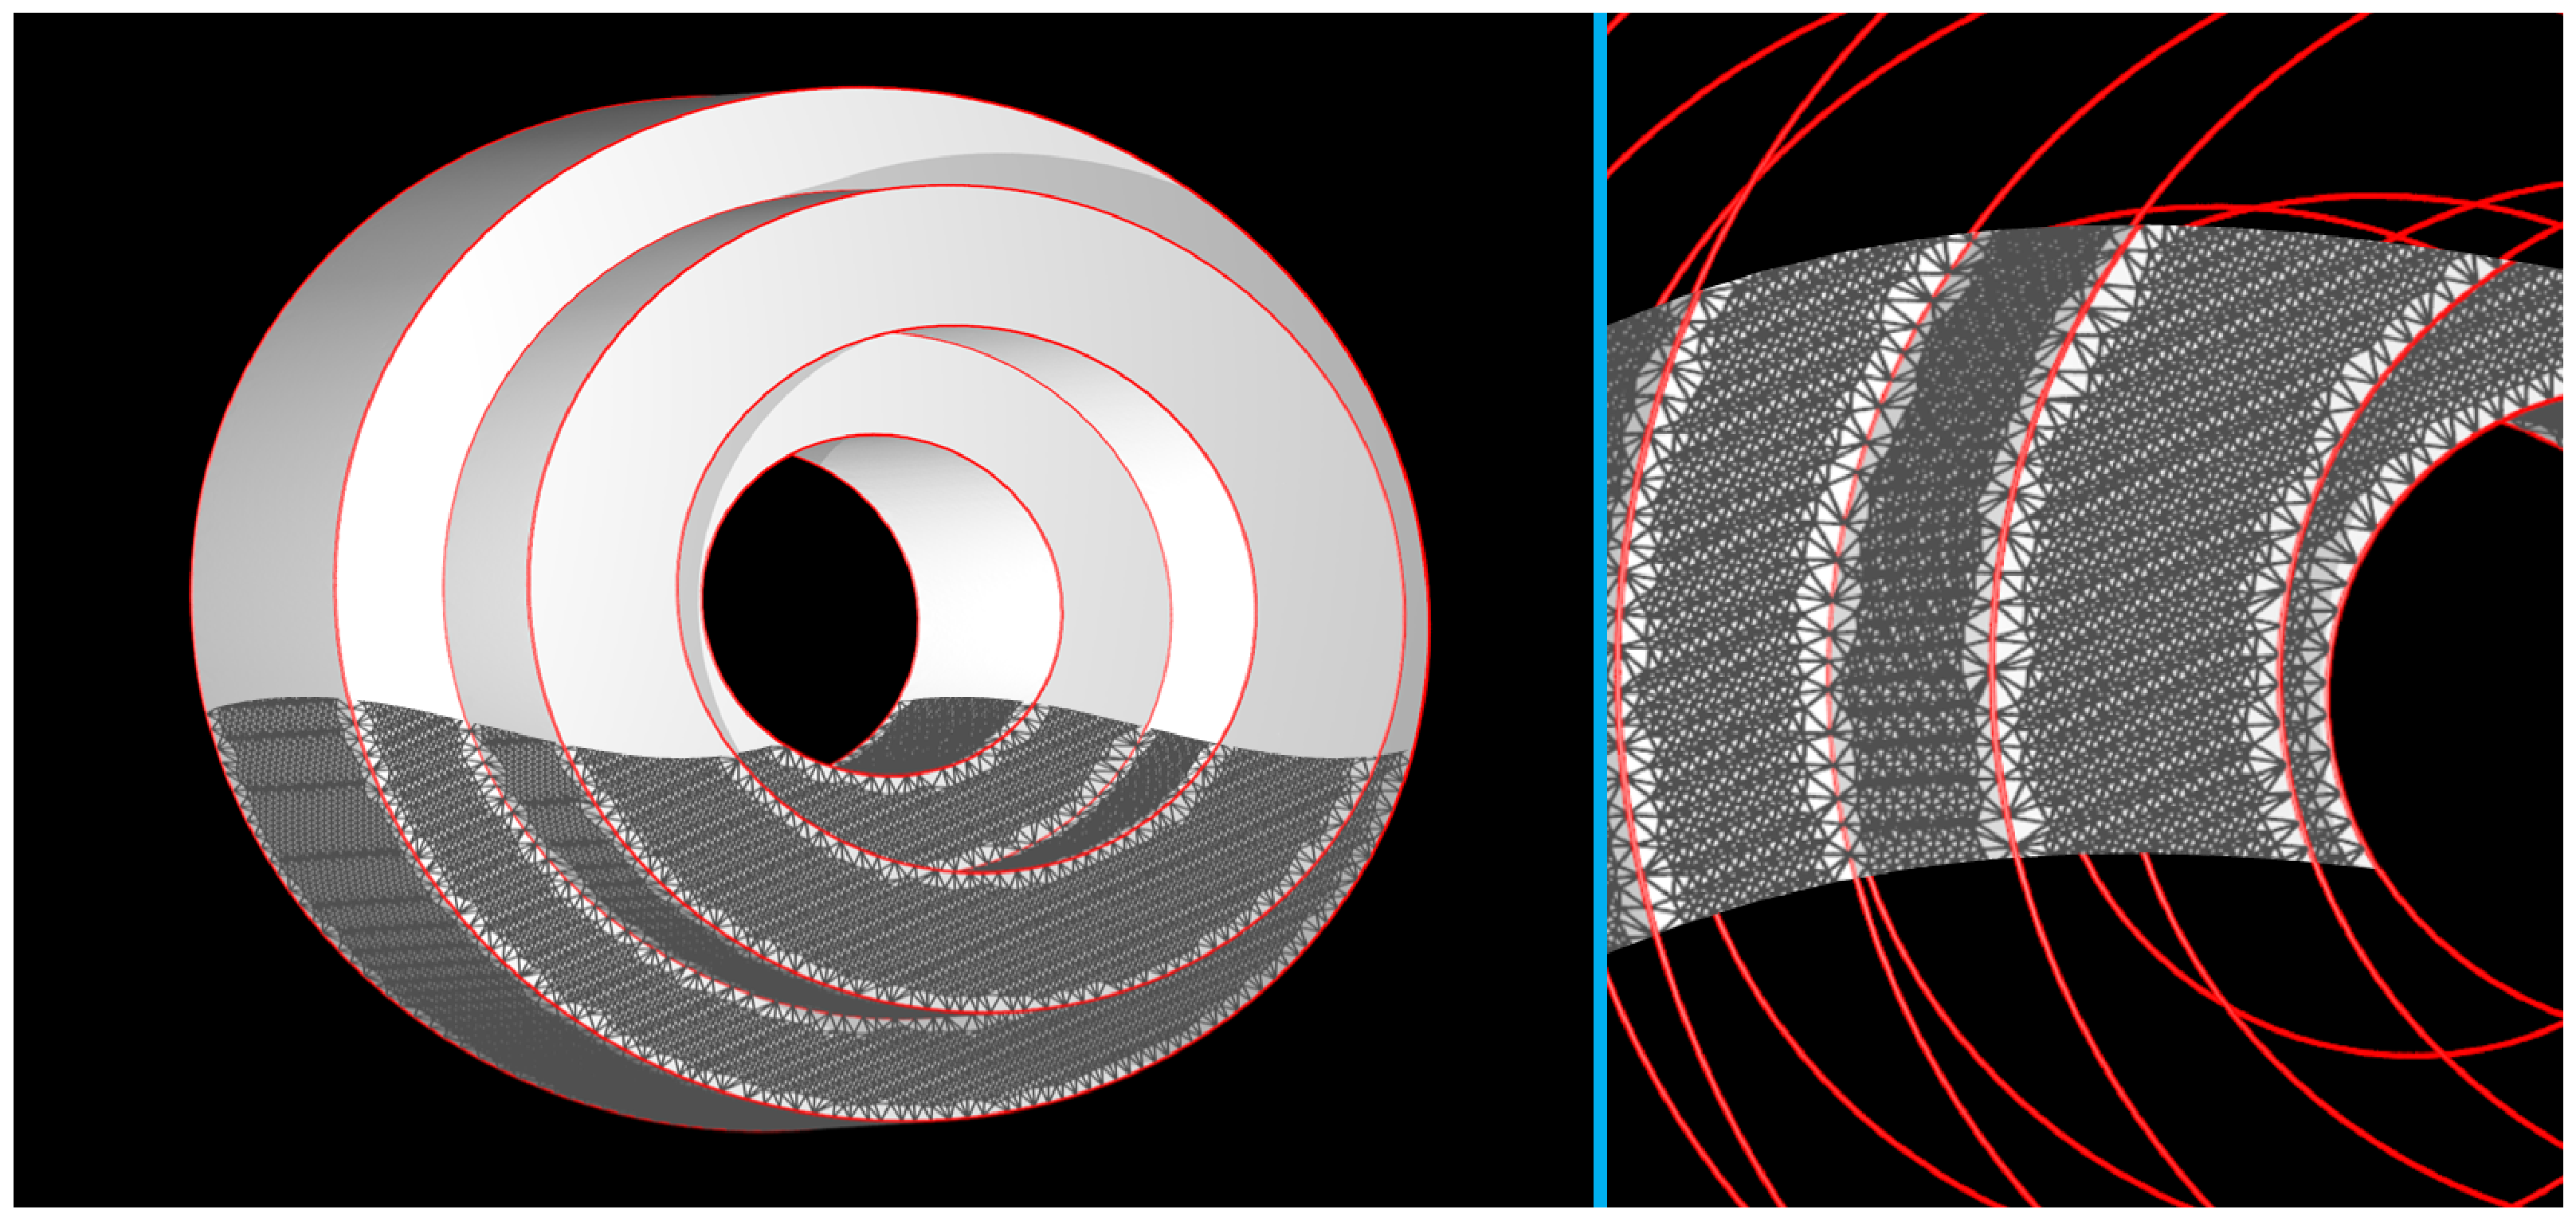
\includegraphics[width=\linewidth]{images/shrecFlangeCombine2.eps}
\caption{Result of SHREC on a Flange dataset. ``Sharp" edges (with dihedral angle less than $140^\circ$) are marked in red. 
``Smooth" edges are in dark grey. The magnified region shows a blend of the ``sharp" edges with a subset of the ``smooth" edges.}
\label{fig:flange1}
\end{figure}
\begin{figure*}[htb]
	\subfloat[]{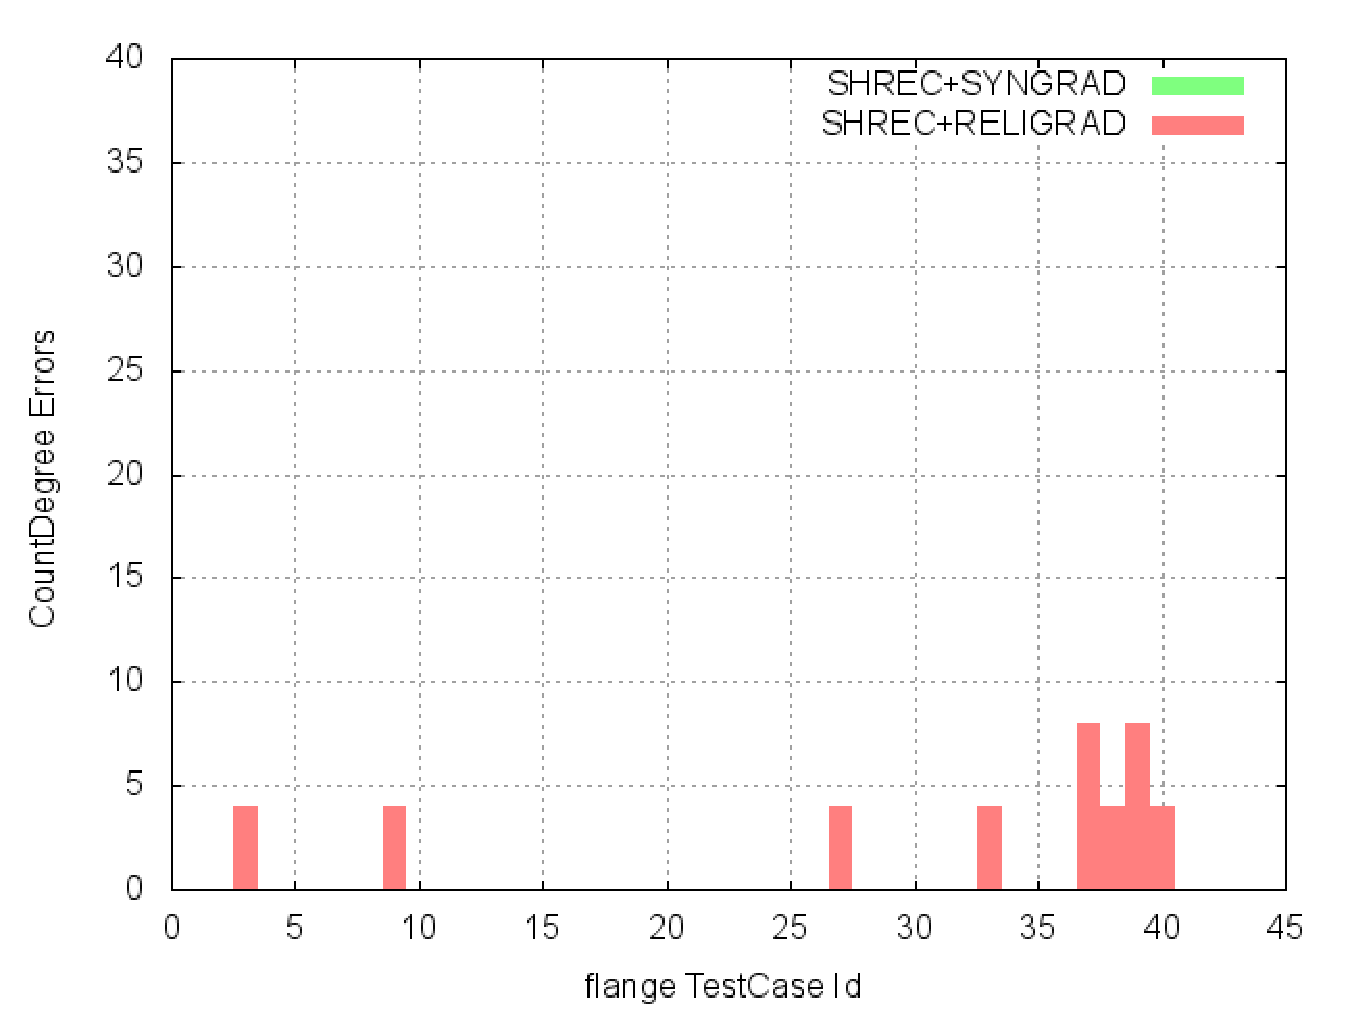
\includegraphics[width=0.33\linewidth]{images/flangeAngle3b.eps}\label{fig:flangeAngle3}}
	\subfloat[]{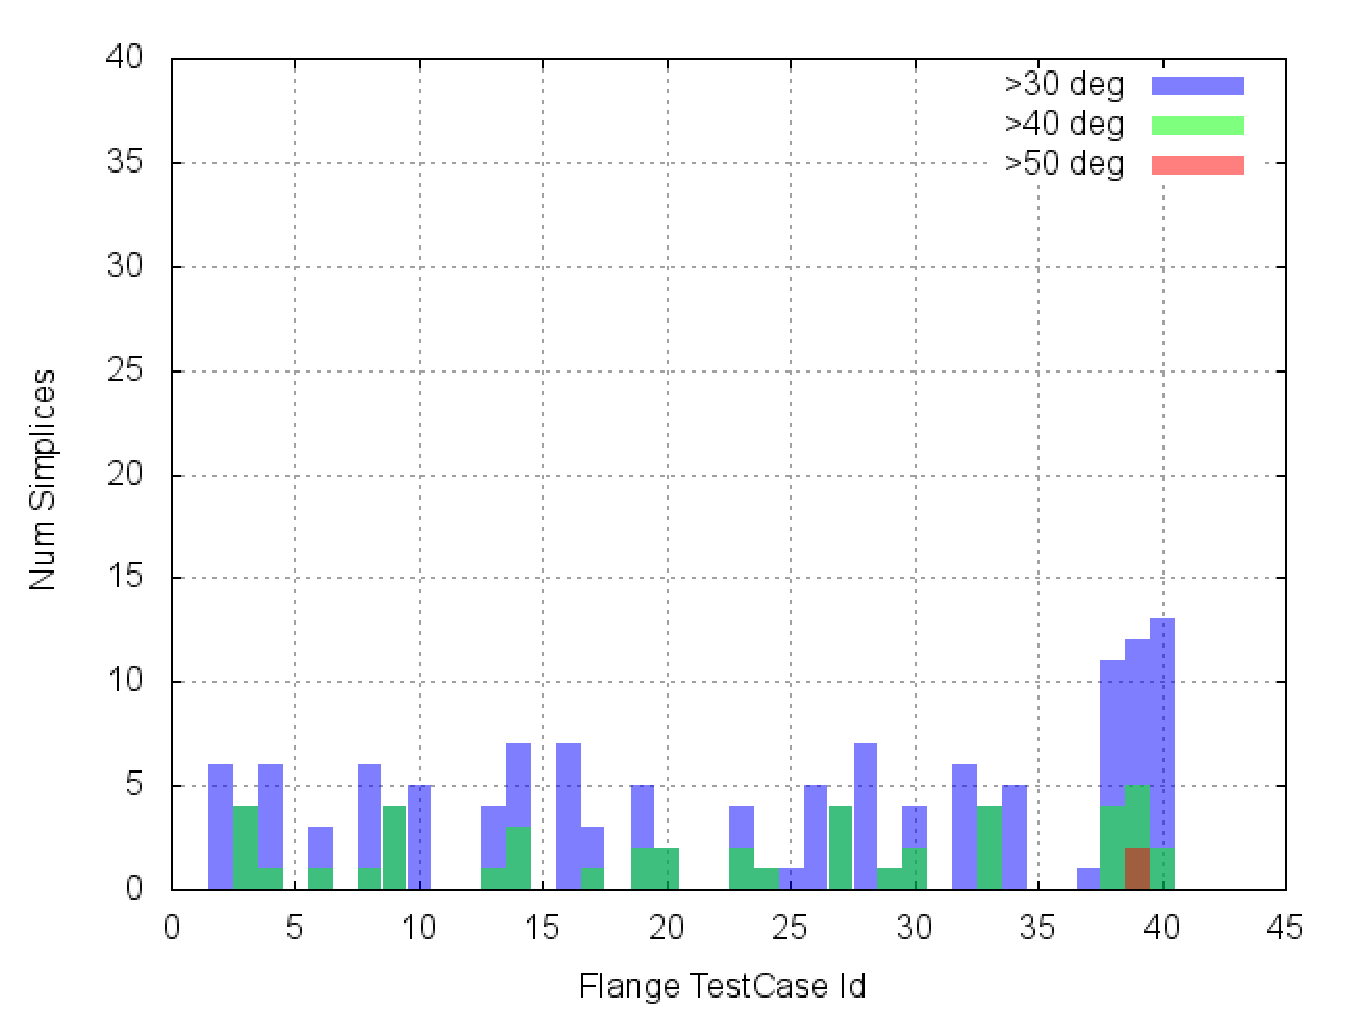
\includegraphics[width=0.33\linewidth]{images/flangeAngle1b.eps}\label{fig:flangeAngle1}}
	\subfloat[]{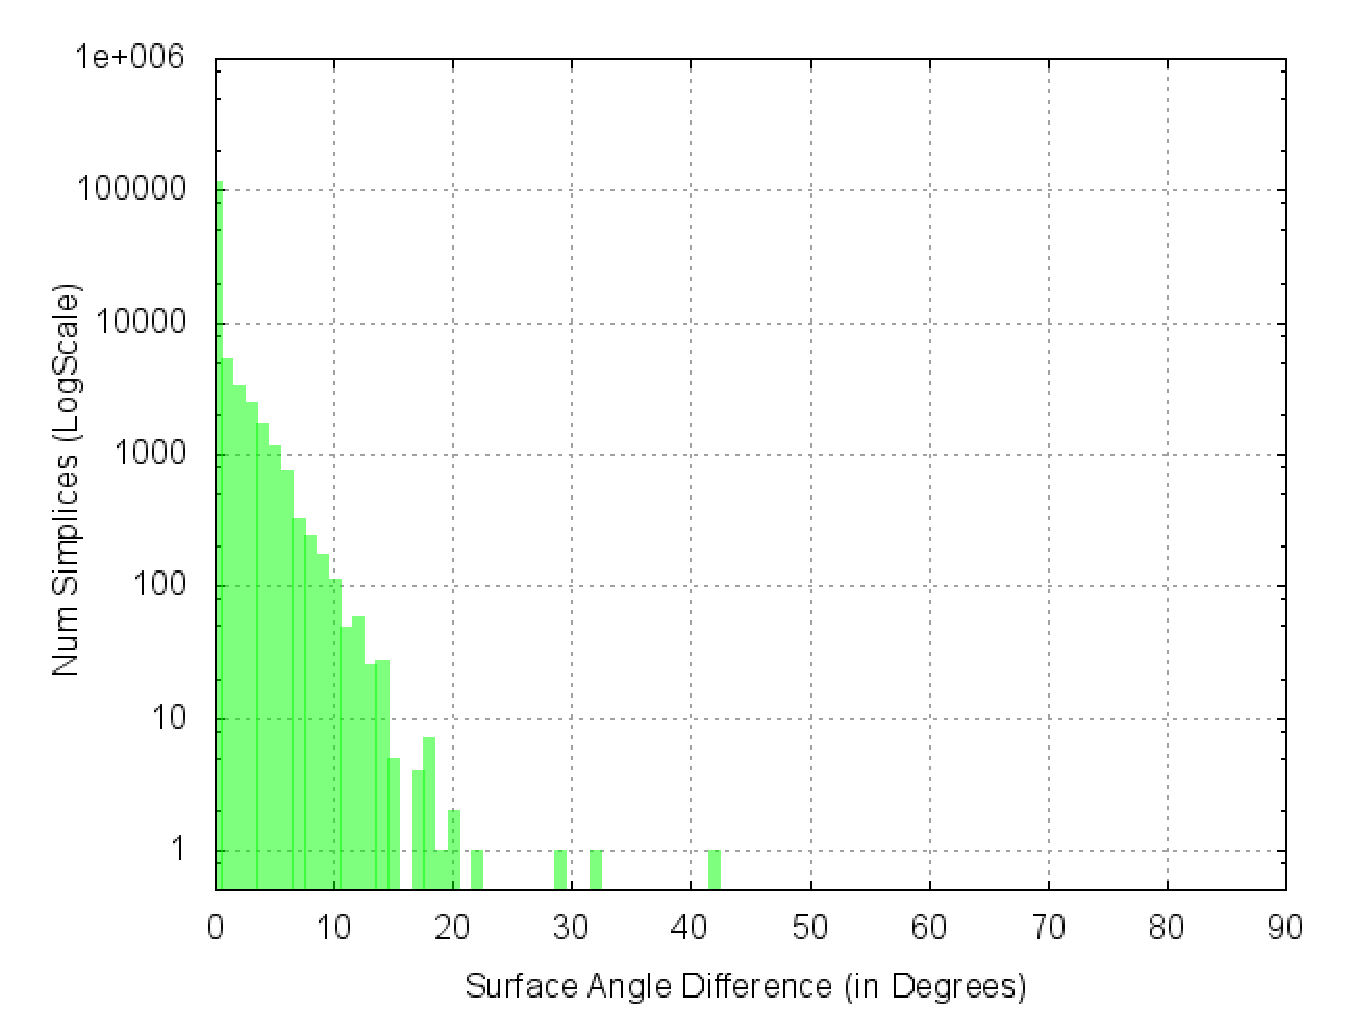
\includegraphics[width=0.33\linewidth]{images/flangeAngle2.eps}\label{fig:flangeAngle2}}
	\caption{SHREC with gradients computed from scalar data using RELIGRAD on 40  FLANGE datasets. (a) Number of CountDegree errors. (b) Number of simplices with angle difference to ``perfect" mesh above 30, 40 and 50 degrees. (b) Shows the angle distribution of one particular case (16) which has three simplices over 30 degrees and 1 above 40 degrees. Total number of simplices is ~133k.}\label{fig:flangeAngle}
\end{figure*}
%\begin{figure*}[p] 
%	\centering
%	\subfloat[]{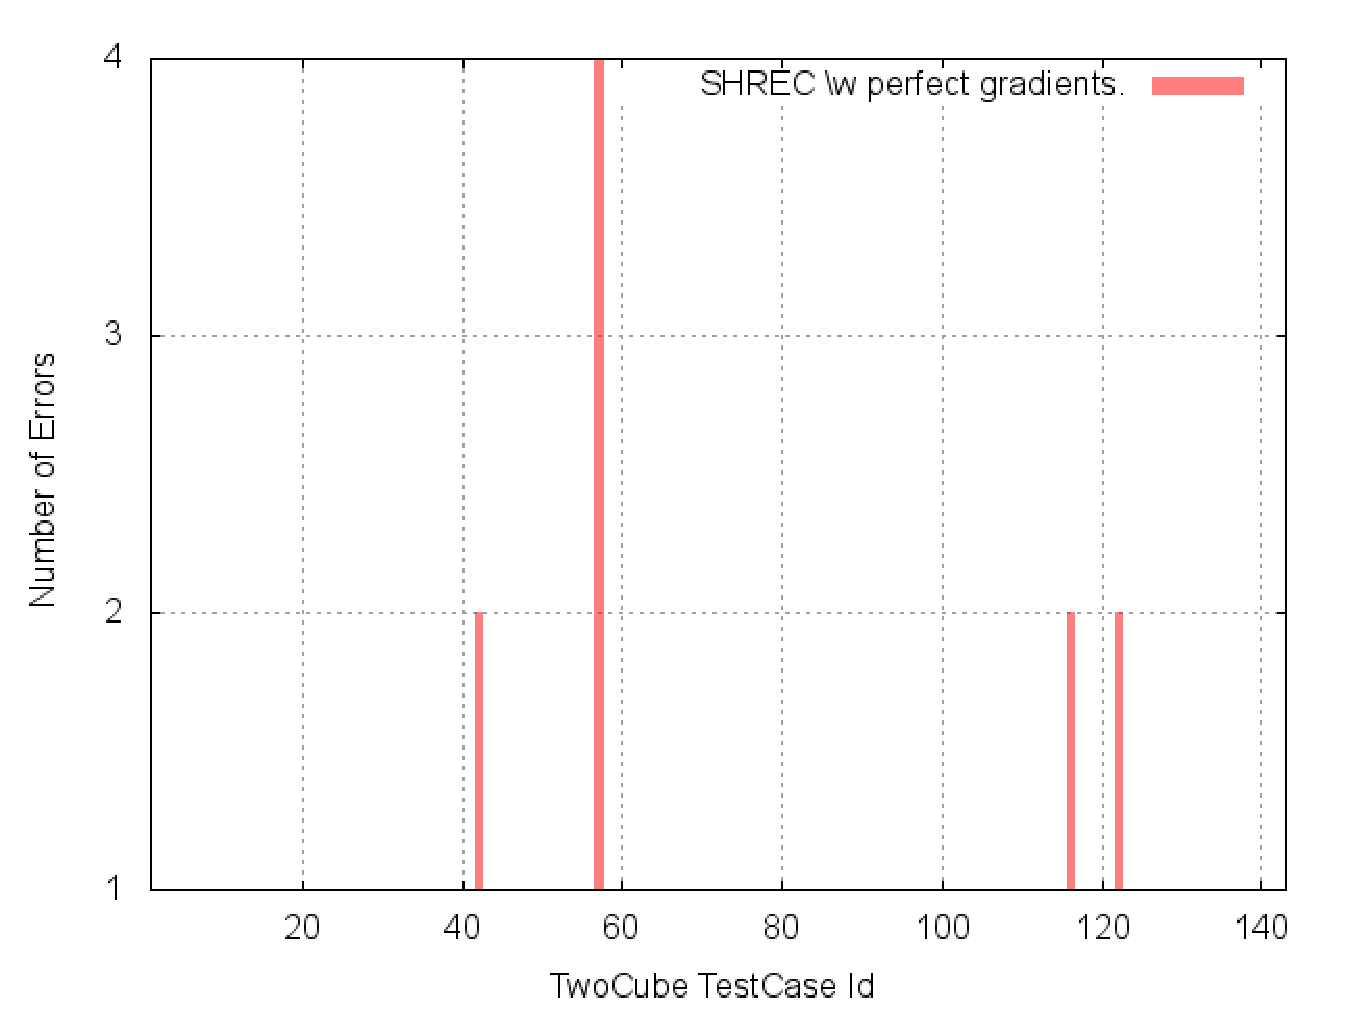
\includegraphics[width=0.5\linewidth]{images/shrecResCol1.eps}\label{fig:shrecTwoCube:a}}
%	\subfloat[]{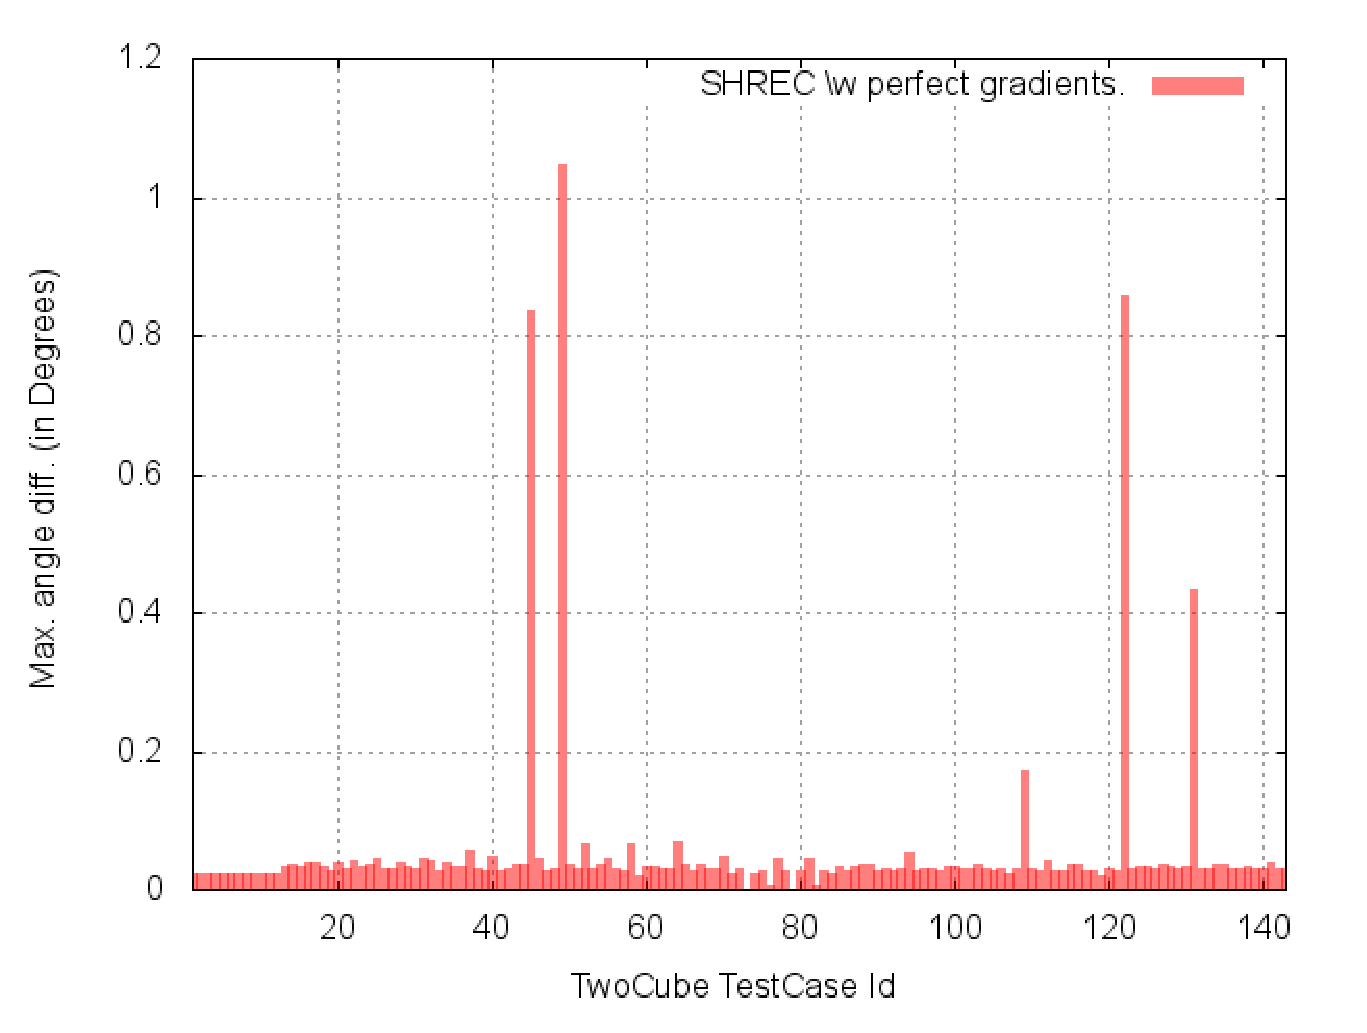
\includegraphics[width=0.5\linewidth]{images/shrecResCol3.eps}\label{fig:shrecTwoCube:b}}\\
%	\subfloat[]{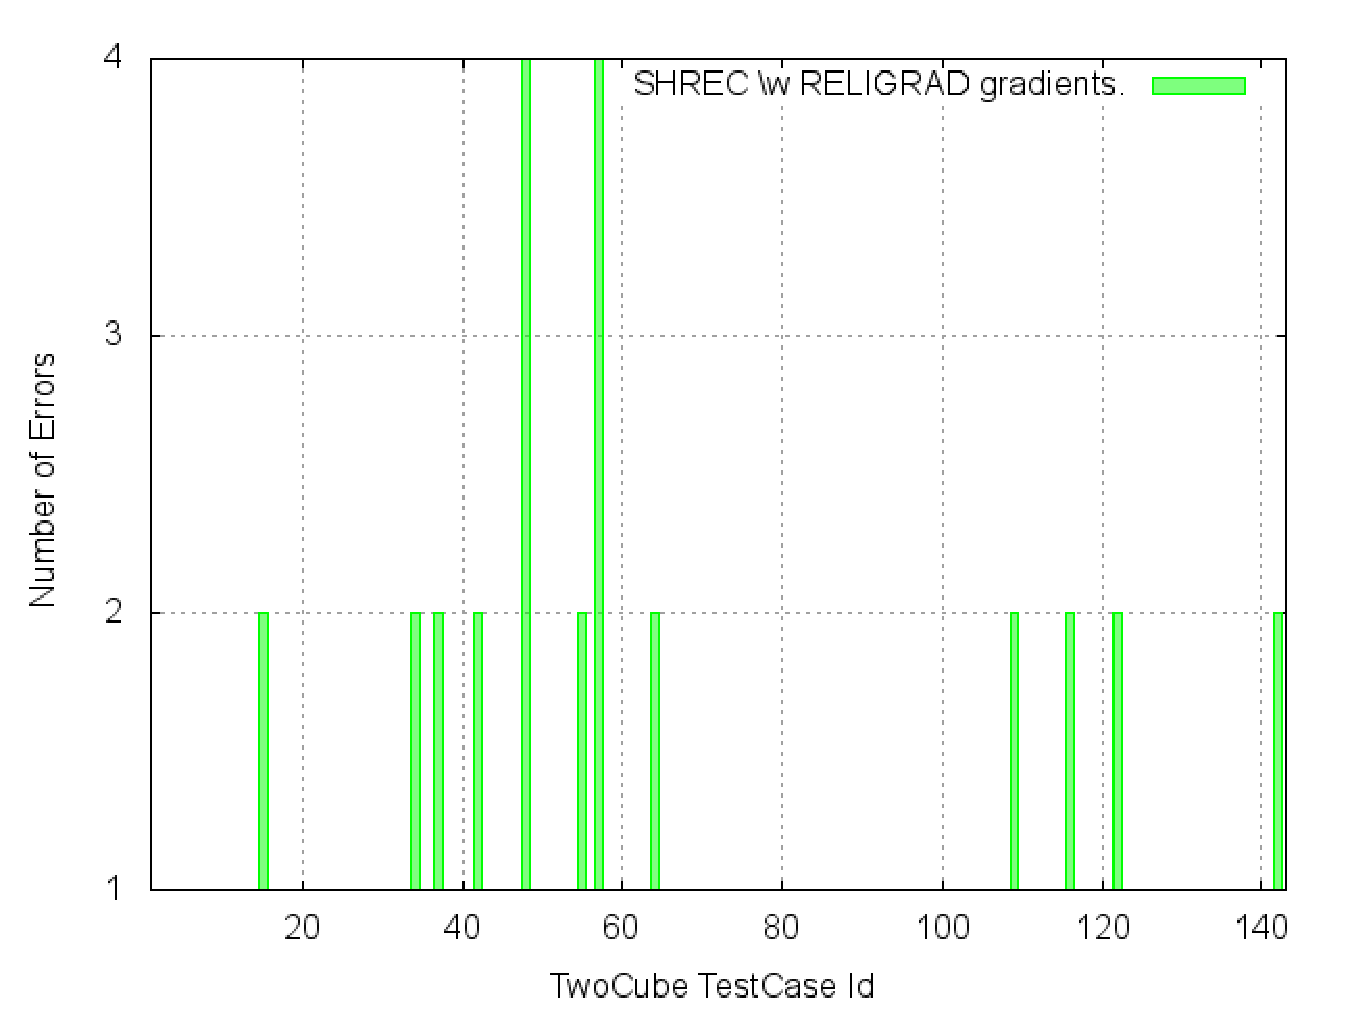
\includegraphics[width=0.5\linewidth]{images/shrecResCol2.eps}\label{fig:shrecTwoCube:c}}
%	\subfloat[]{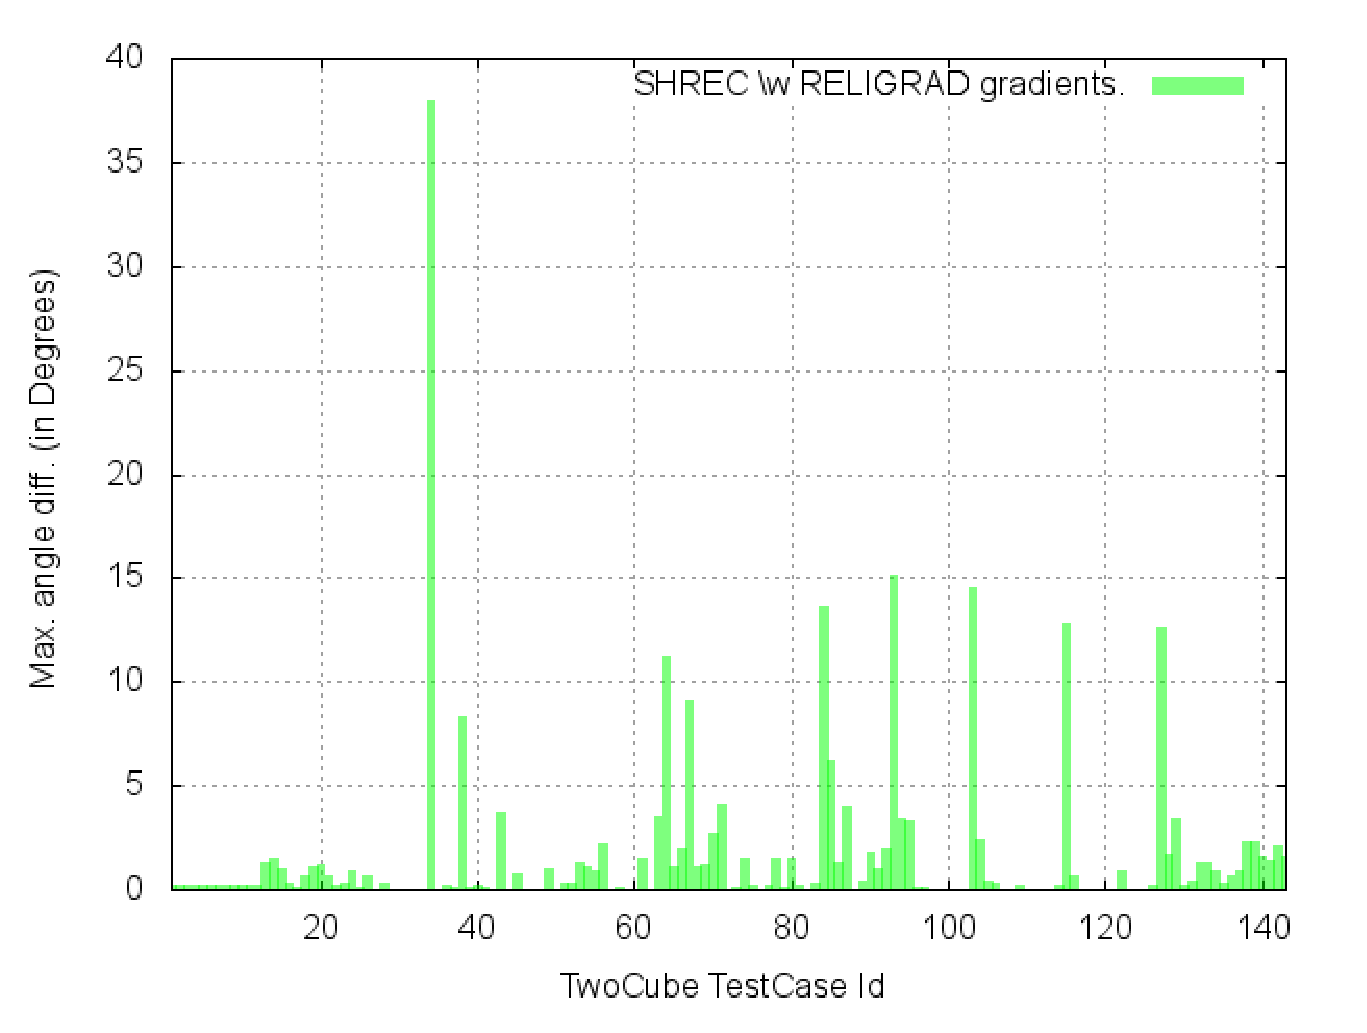
\includegraphics[width=0.5\linewidth]{images/shrecResCol4.eps}\label{fig:shrecTwoCube:d}}
%	\caption{SHREC with perfect gradients and with RELIGRAD gradients(computed directly from scalar data.).~\protect\subref{fig:shrecTwoCube:a} shows the number of CountDegree errors when using SHREC along with the correct gradients.~\protect\subref{fig:shrecTwoCube:c} The same result when using gradients computed directly from scalar data (RELIGRAD). ~\protect\subref{fig:shrecTwoCube:b} shows the maximum angle difference from the ``perfect mesh" when using correct gradients.~\protect\subref{fig:shrecTwoCube:d} The same result when using RELIGRAD gradients. }
%	\label{fig:shrecTwoCube}
%	\vskip-0.2cm
%\end{figure*}
\begin{figure*}
	\centering	
	\subfloat[SHREC+ synthetic Gradients]{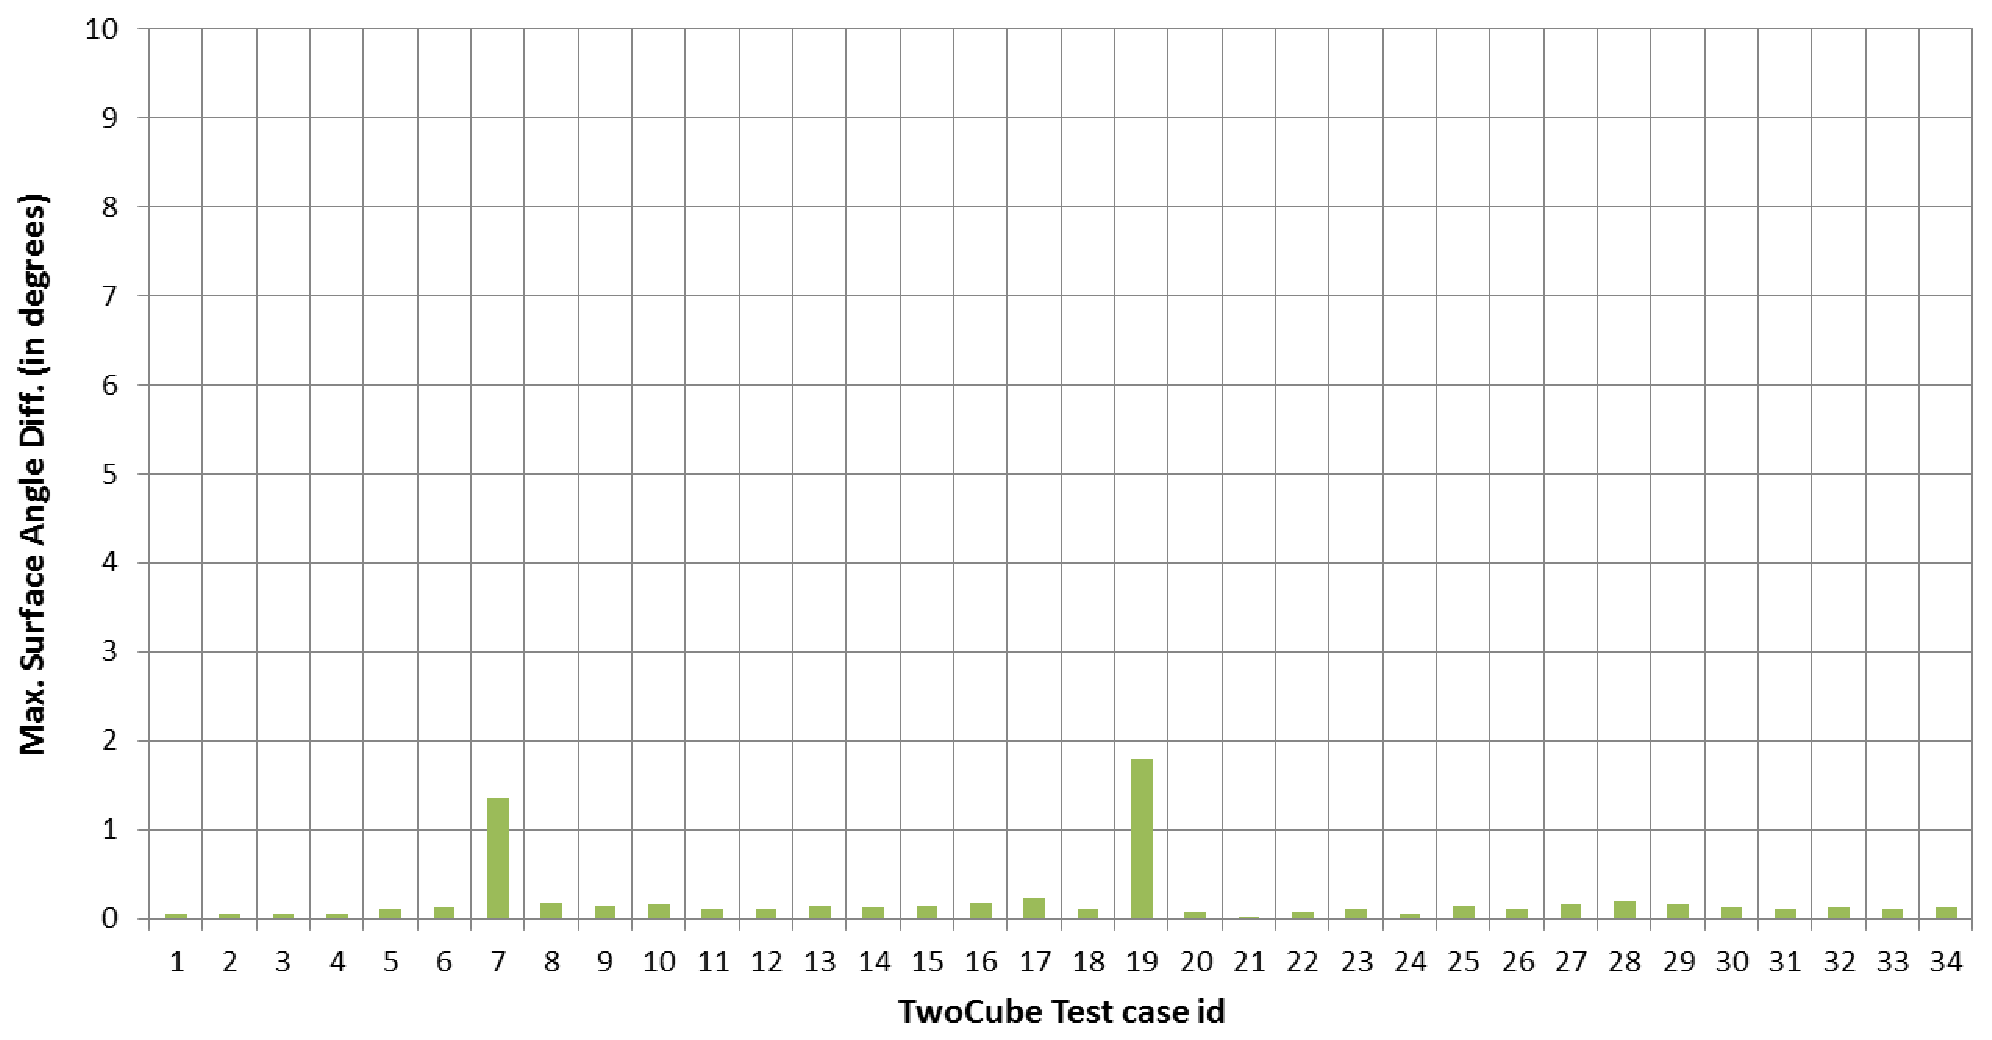
\includegraphics[width=0.45\linewidth]{images/tw1.eps}
		\label{fig:summ_tw:a}}\quad
	\subfloat[SHREC+ RELIGRAD Gradients]{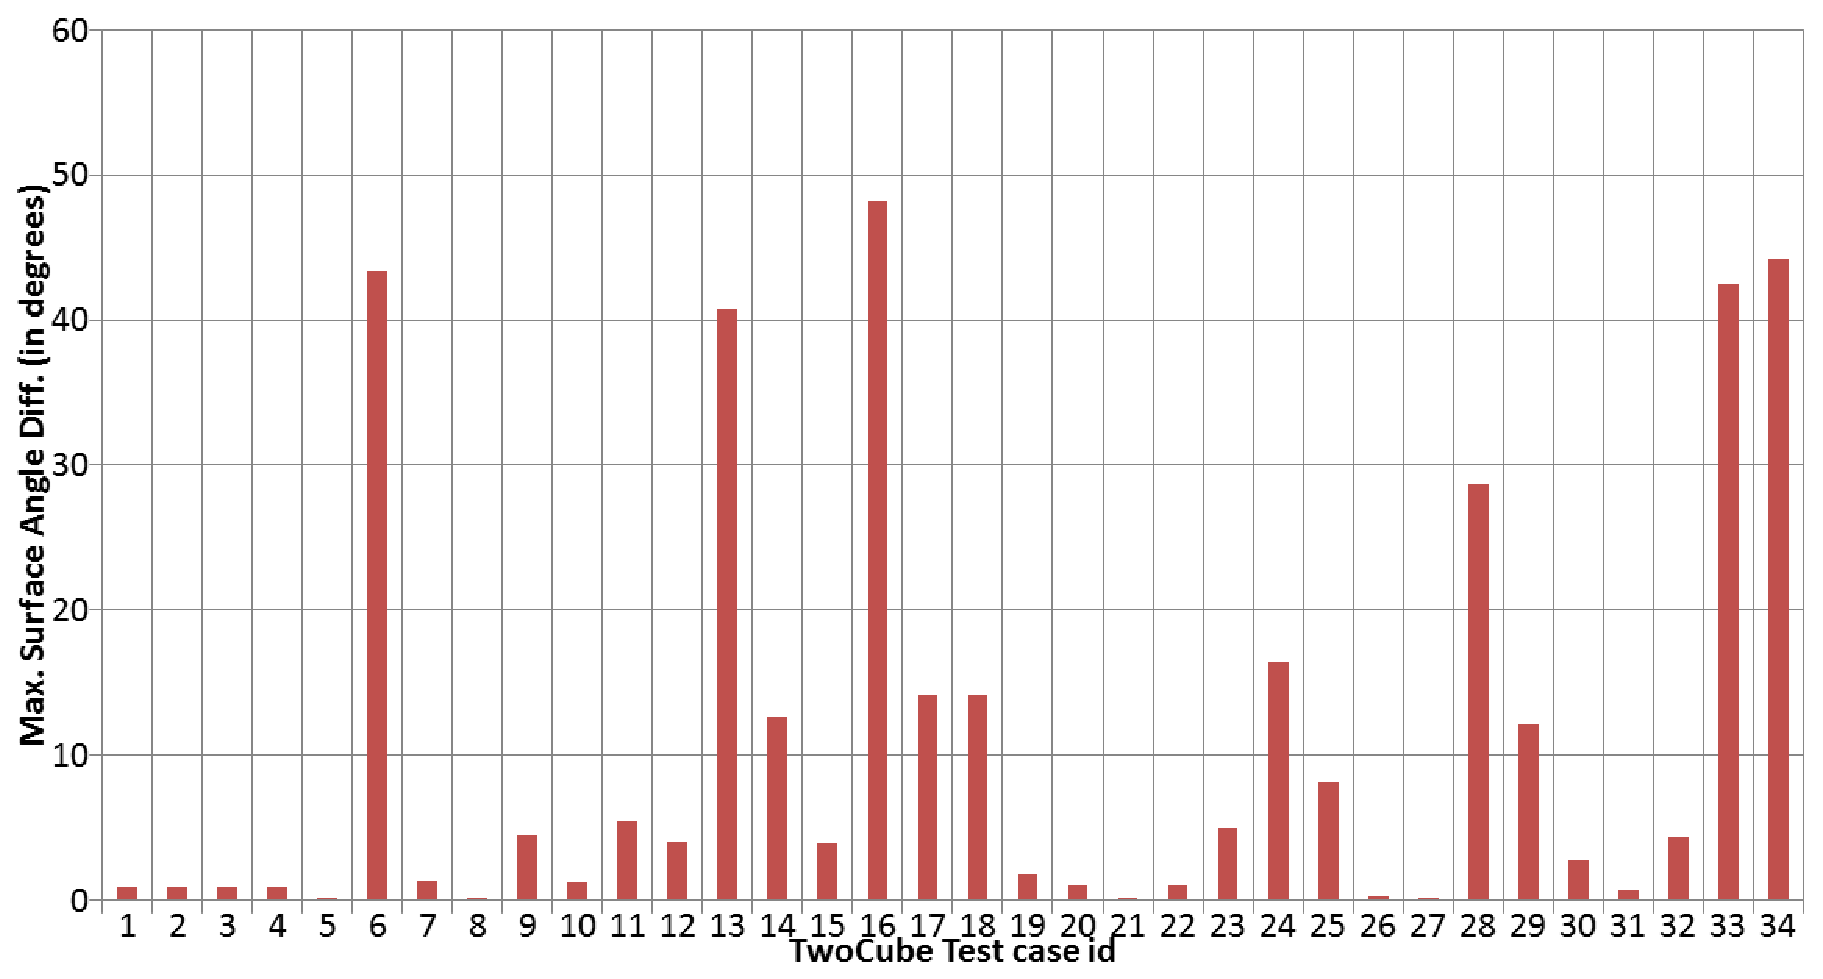
\includegraphics[width=0.45\linewidth]{images/tw2.eps}
		\label{fig:summ_tw:b}}\\
	\subfloat[SHREC+ RELIGRAD Gradients]{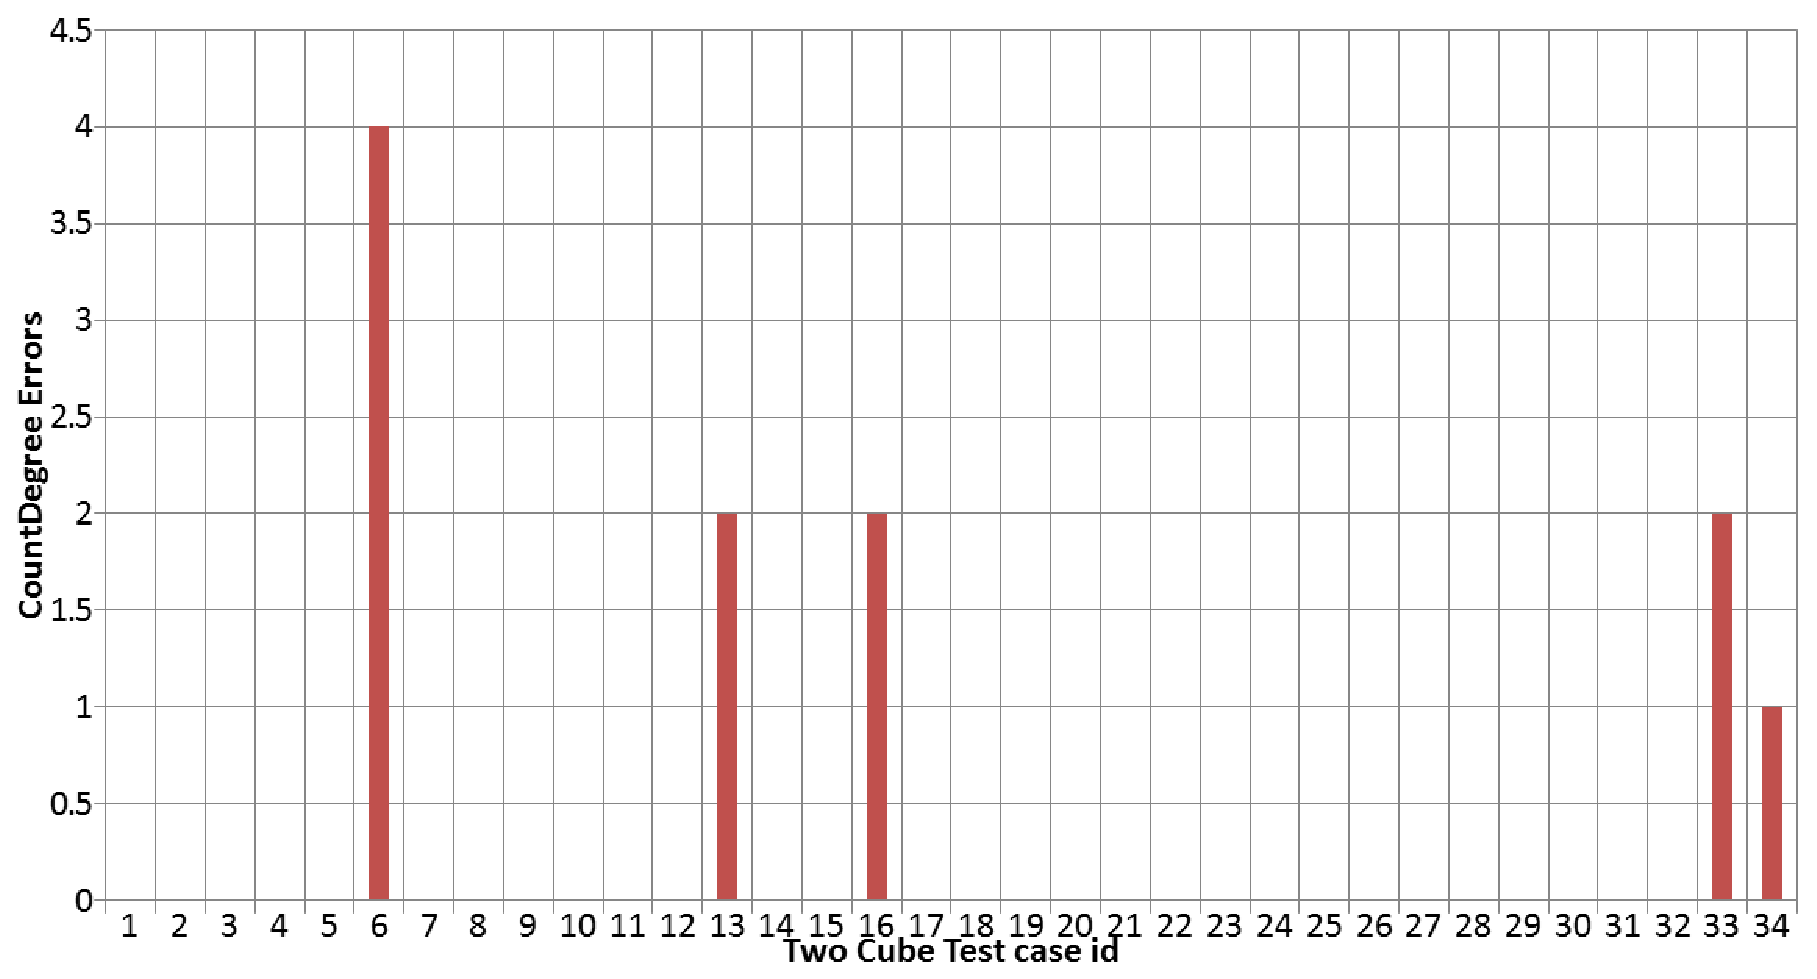
\includegraphics[width=0.45\linewidth]{images/tw3.eps}
		\label{fig:summ_tw:c}}\quad
	\subfloat[SHREC+ RELIGRAD Gradients]{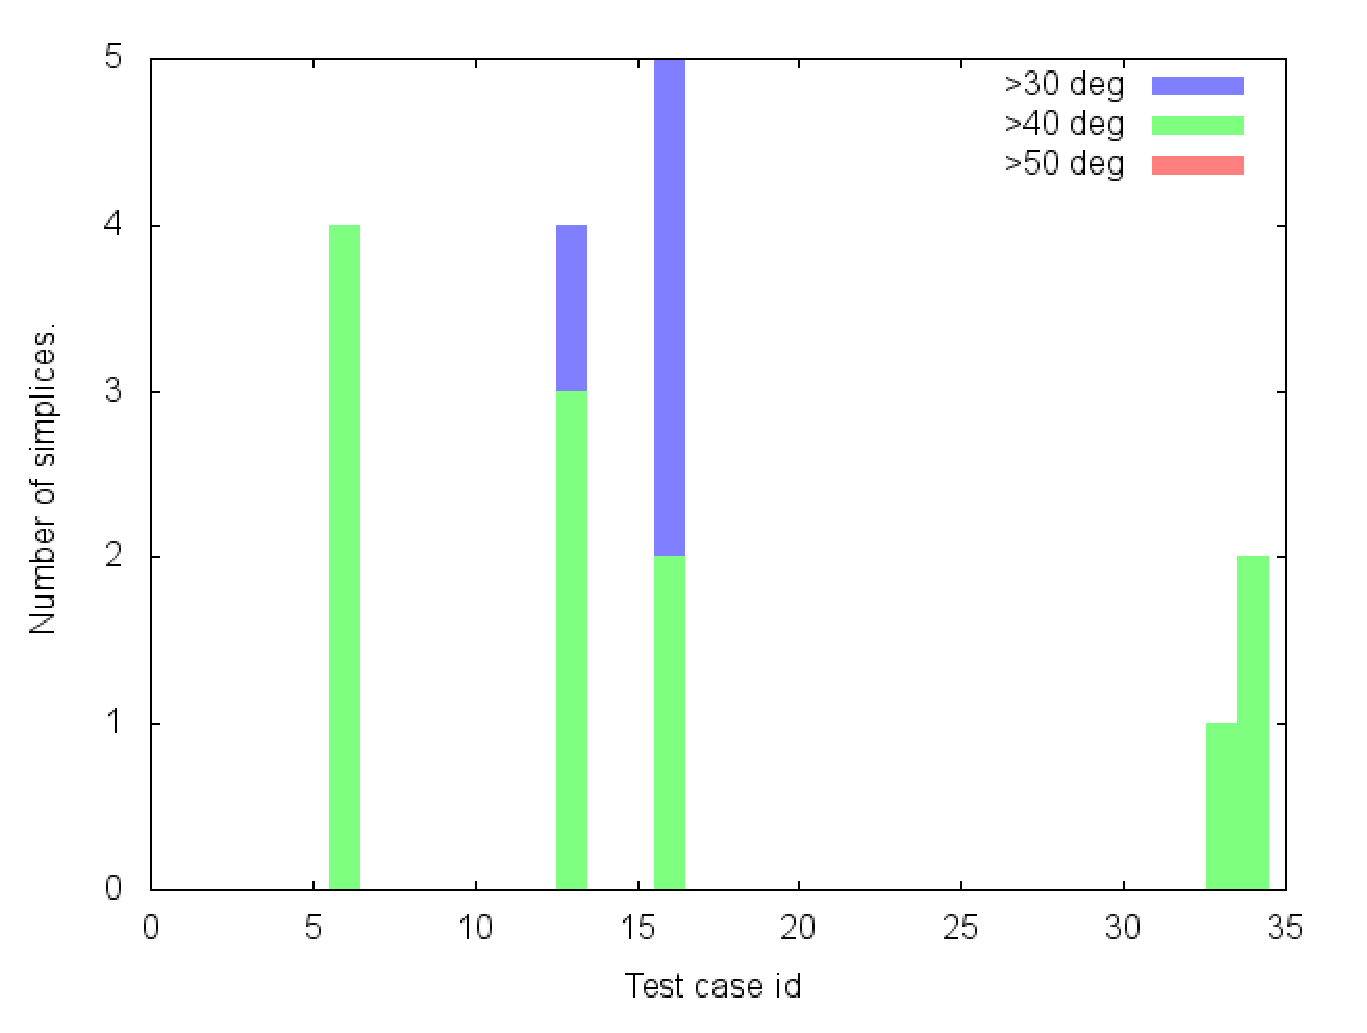
\includegraphics[height=0.25\linewidth]{images/twoCube35_test_1.eps}
		\label{fig:summ_tw:d}}
	\caption{SHREC summary results on 34 twocube datasets. Figure~\protect\subref{fig:summ_tw:a} shows the maximum surface angle difference from the synthetic meshes when using SHREC with synthetic gradients. Figure~\protect\subref{fig:summ_tw:b} shows the maximum surface angle difference for the same test cases when using SHREC with RELIGRAD gradients. Figure~\protect\subref{fig:summ_tw:c} shows the countDegree errors when using SHREC with RELIGRAD gradients. 
	Figure~\protect\subref{fig:summ_tw:d} shows the number of simplices with surface angle difference more than 30, 40, 50$^{\circ}$ for SHREC running with RELIGRAD. 
	 Note: SHREC with synthetic gradients produces "NO" countDegree errors and the maximum surface angle error (Fig.~\protect\subref{fig:summ_tw:a}) is less than 1.8$^{\circ}$, to small to show angle distribution. }
	\label{fig:shrecTwoCube}
\end{figure*}


We next ran SHREC on 34 TwoCube datasets once again with different orientations. Figure~\ref{fig:shrecTwoCube} shows the summary results. As with Flange we first tested SHREC with synthetic gradients and then with gradients computed from the scalar data using RELIGRAD.

On the 34 twoCube datasets, SHREC with synthetic gradients generated no countDegree errors. 
Figure~\protect\subref*{fig:summ_tw:a} shows the results for maximum surface angle difference from the synthetic mesh, using the SHREC algorithm along with synthetic gradients as input. The reconstructions are very accurate, the maximum angle difference was less than 2$^{\circ}$. 

Next we discuss results with SHREC using gradients generated using RELIGRAD;
Figure~\protect\subref*{fig:summ_tw:b}, shows the maximum angle difference from the synthetic mesh was less than 50$^\circ$ (id 16). CountDegree summary (Figure~\protect\subref*{fig:summ_tw:c}) shows that only 5 out of 34 datasets, had errors with a maximum of 4. Figure~\protect\subref*{fig:summ_tw:d} shows that dataset (id 16) which had the maximum surface angle difference error had only 5 simplices with angle difference more than 30$^\circ$ and a single simplex over 40$^\circ$.
Figure~\ref{fig:shrecPerfect1} shows the mesh and the edges generated on a particular dataset.

Results of running SHREC with RELIGRAD on 15 Cannon datasets  with different orientations are shown in Figure~\protect\subref*{fig:cannon:b},~\protect\subref*{fig:cannon:a}. Figure~\protect\subref*{fig:cannon:b} shows the CountDegree errors generated for the 15 cannon sets using gradients computed from RELIGRAD, the maximum error generated was 2. SHREC using synthetic gradients generated 'NO' errors. Figure~\protect\subref*{fig:cannon:a} shows one representative result using SHREC and RELIGRAD directly from scalar data. The magnified region shows a portion of the sharp edge. 

Similarly, Figure ~\protect\subref*{fig:cone:b},~\protect\subref*{fig:cone:a} show our results of running SHREC with RELIGRAD and synthetic gradient on the 14 Cone datasets.
SHREC with synthetic gradients generates errors in only two cases with a  maximum of 4 countDegree errors. 
\begin{figure}[tb]
	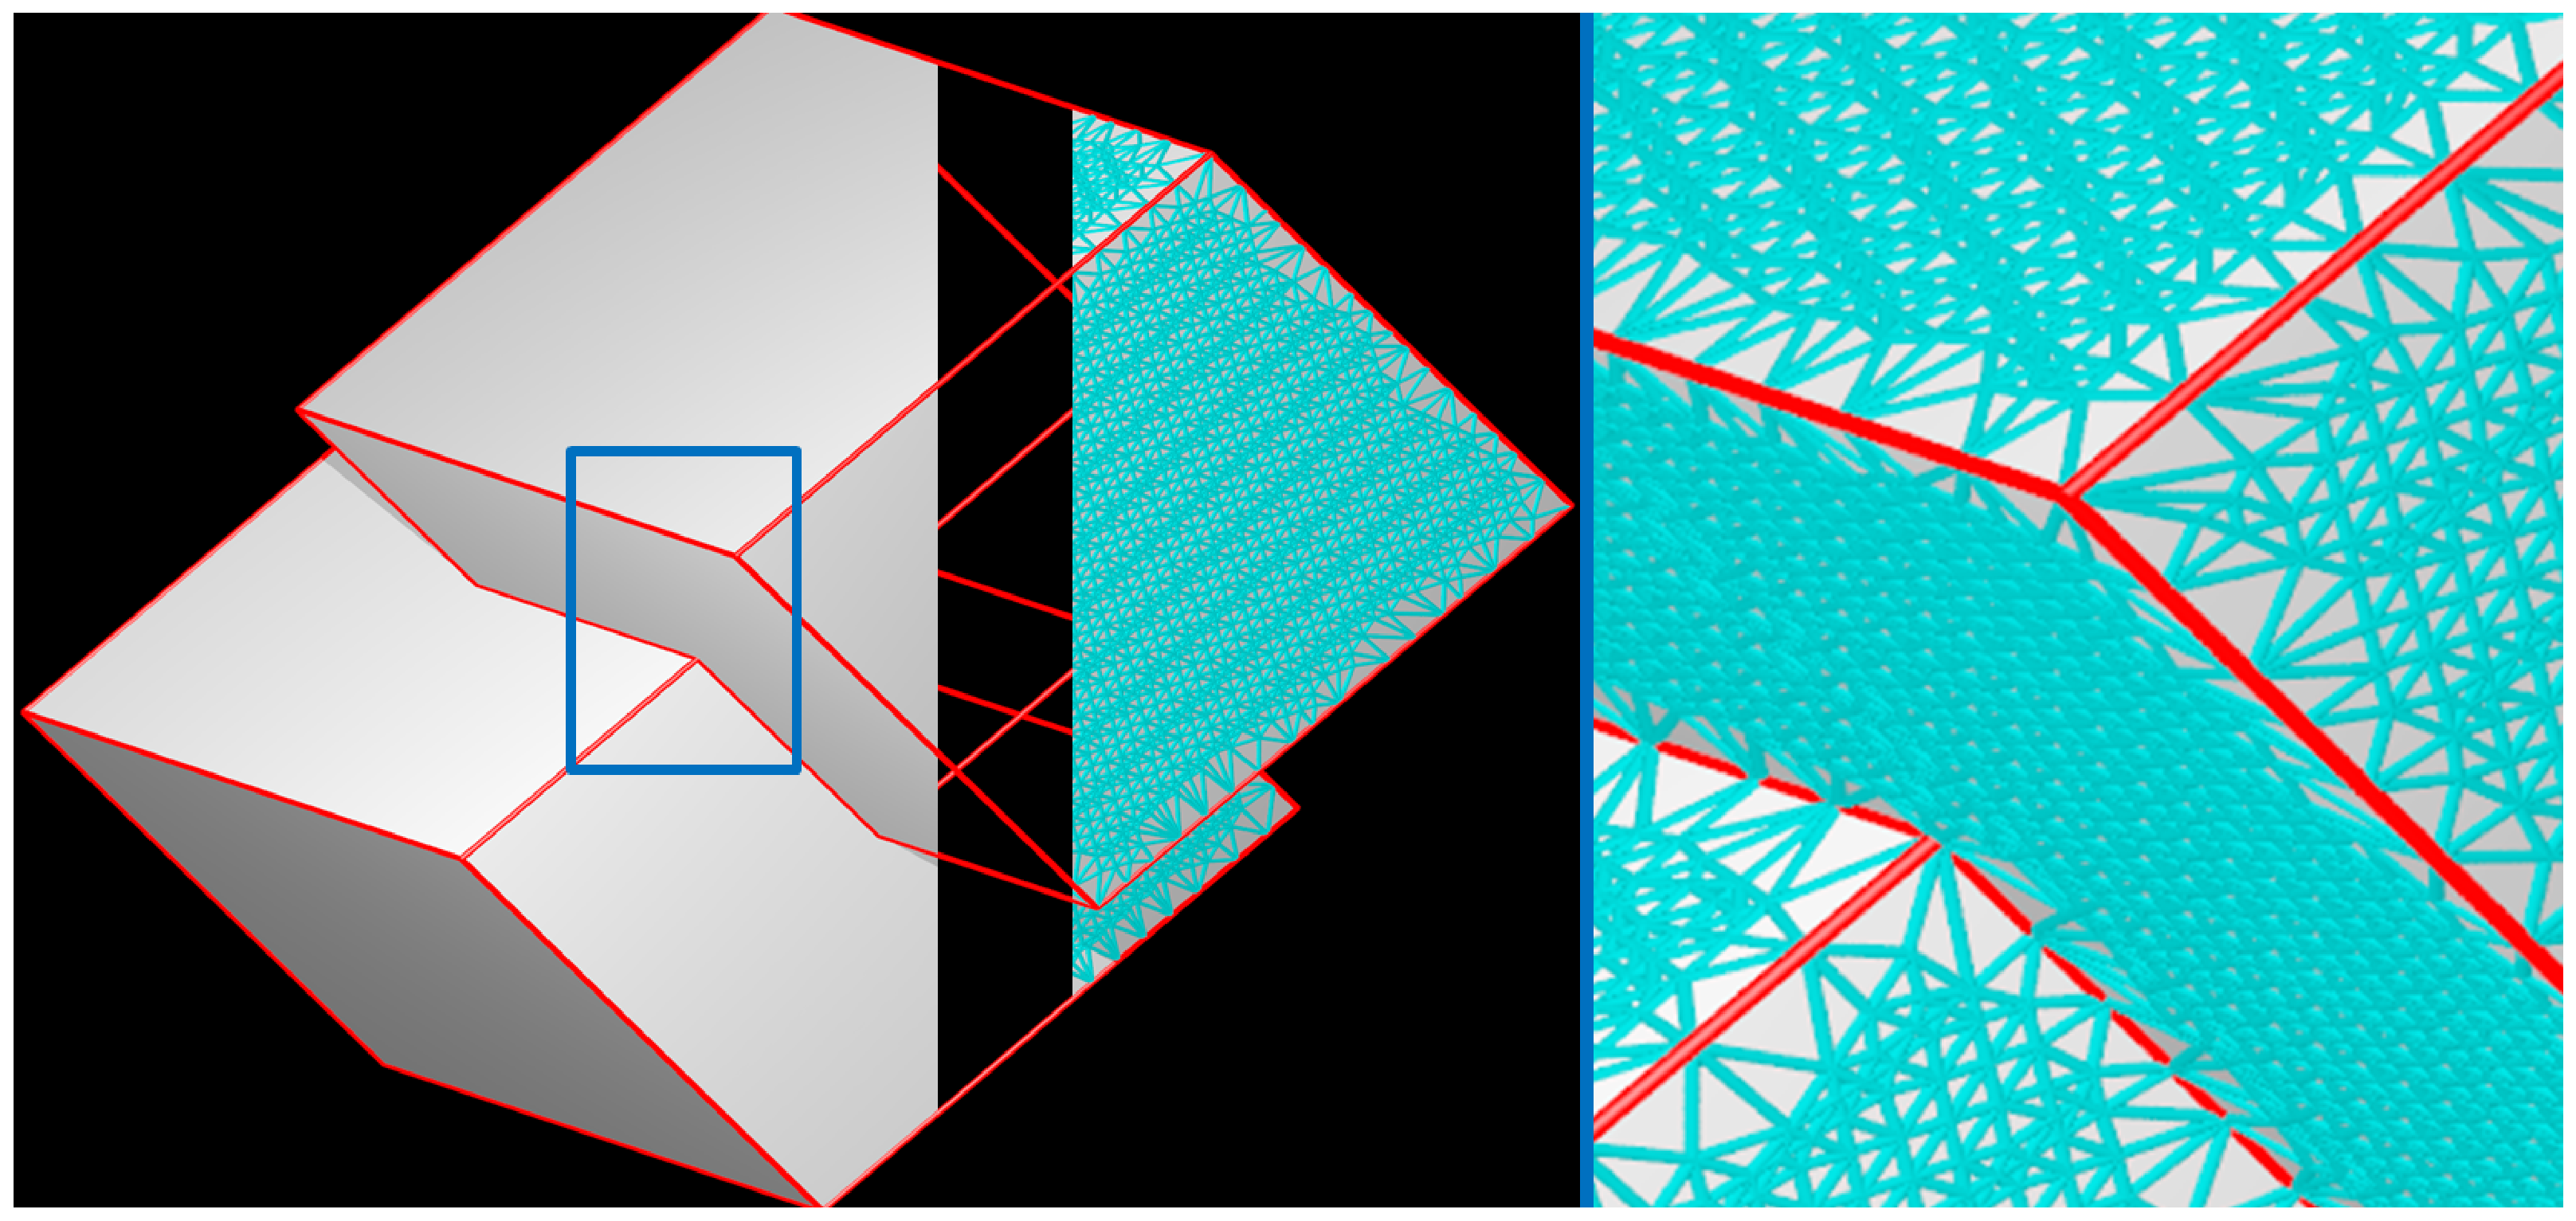
\includegraphics[width=\linewidth]{images/shrecPerfect.eps}
	\caption{Result of SHREC on a twoCube dataset. ``sharp" edges are marked in red. Smooth edges are shown in cyan. The magnified region shows the output mesh edges around a corner.}
	\label{fig:shrecPerfect1}
\end{figure}
\begin{figure}[htb]
	\subfloat[]{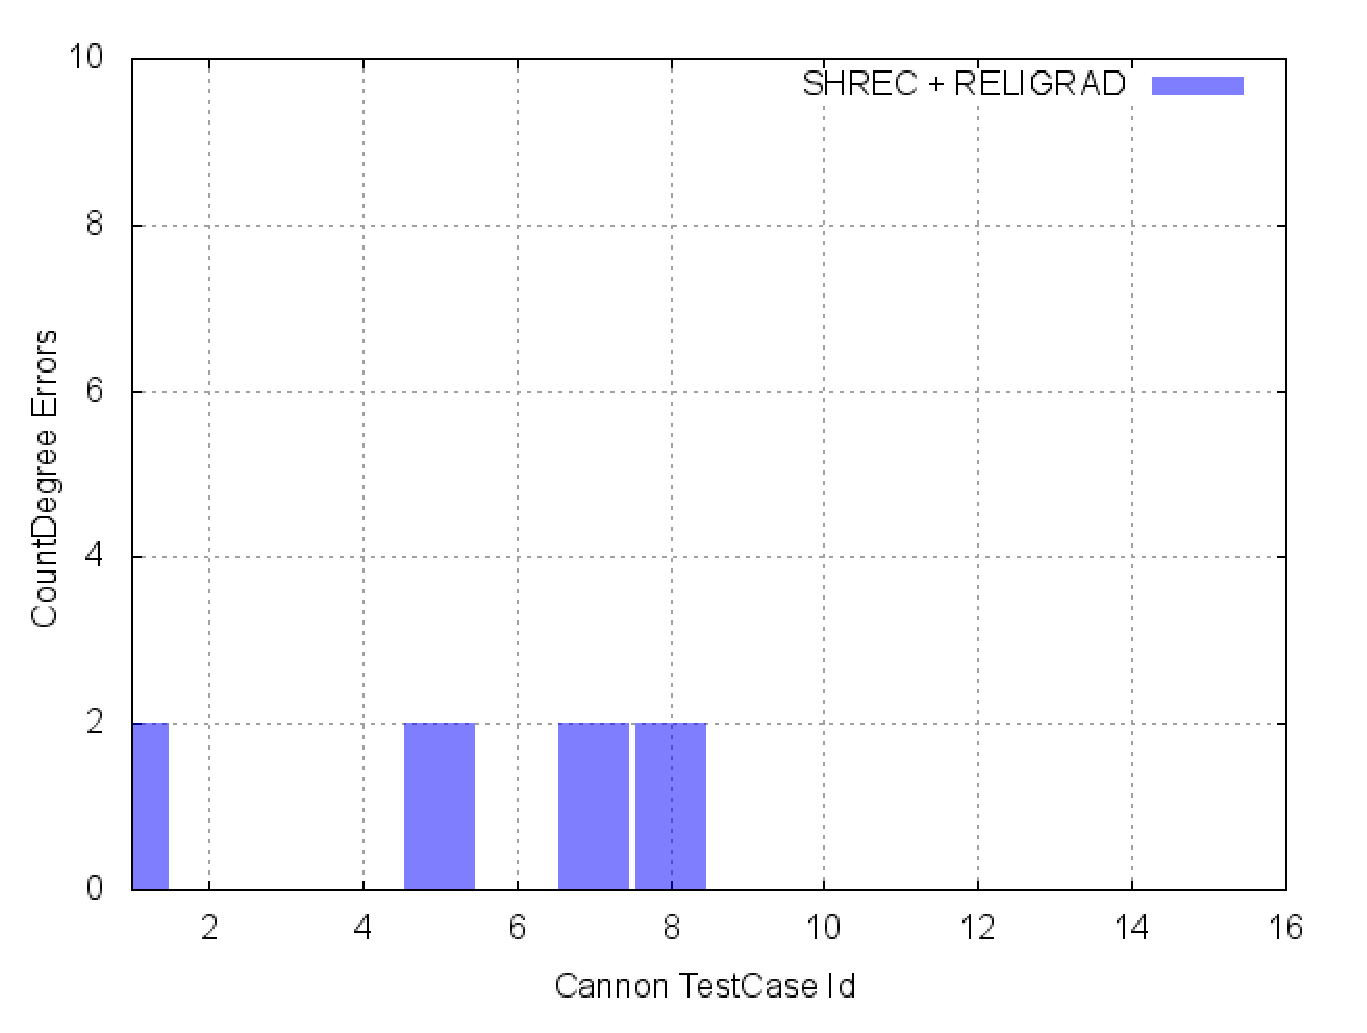
\includegraphics[width=0.5\linewidth]{images/cannon.eps}\label{fig:cannon:b}}
	\subfloat[]{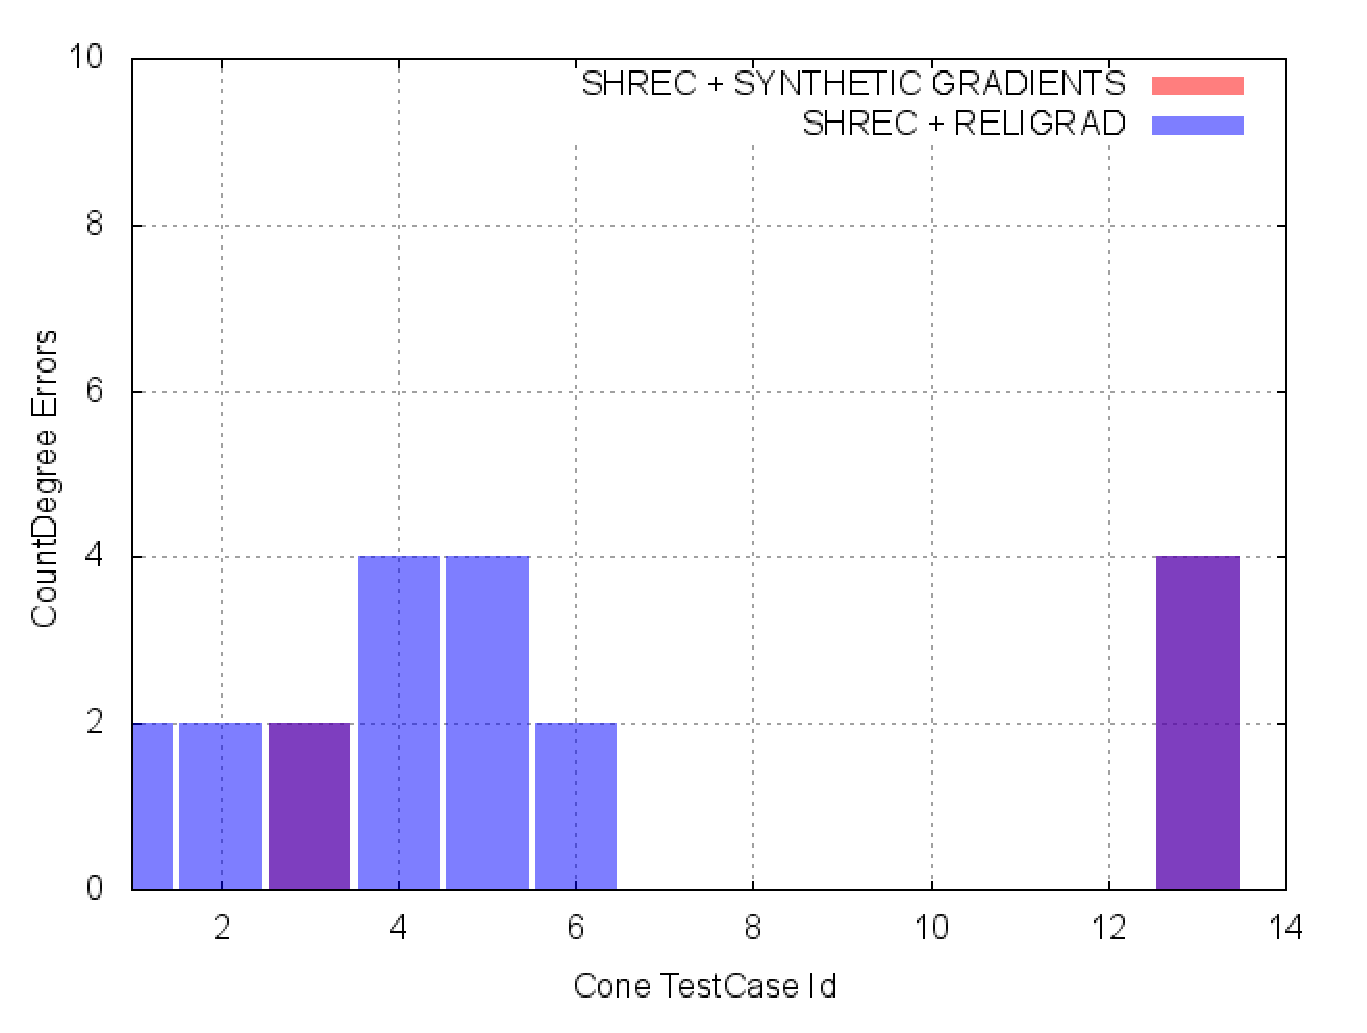
\includegraphics[width=0.5\linewidth]{images/cone.eps}\label{fig:cone:b}}
	\caption{Summary result of algorithm SHREC on Cannon and cone Datasets. (a) CountDegree Errors on 15 Cannon datasets using RELIGRAD gradients. SHREC with synthetic gradients had no errors and is not shown. (b) CountDegree errors on 14 Cone datasets using RELIGRAD and synthetic gradients.}
	\label{fig:cannon_cone_summary}
\end{figure}
\begin{figure}[tb]
	\subfloat[]{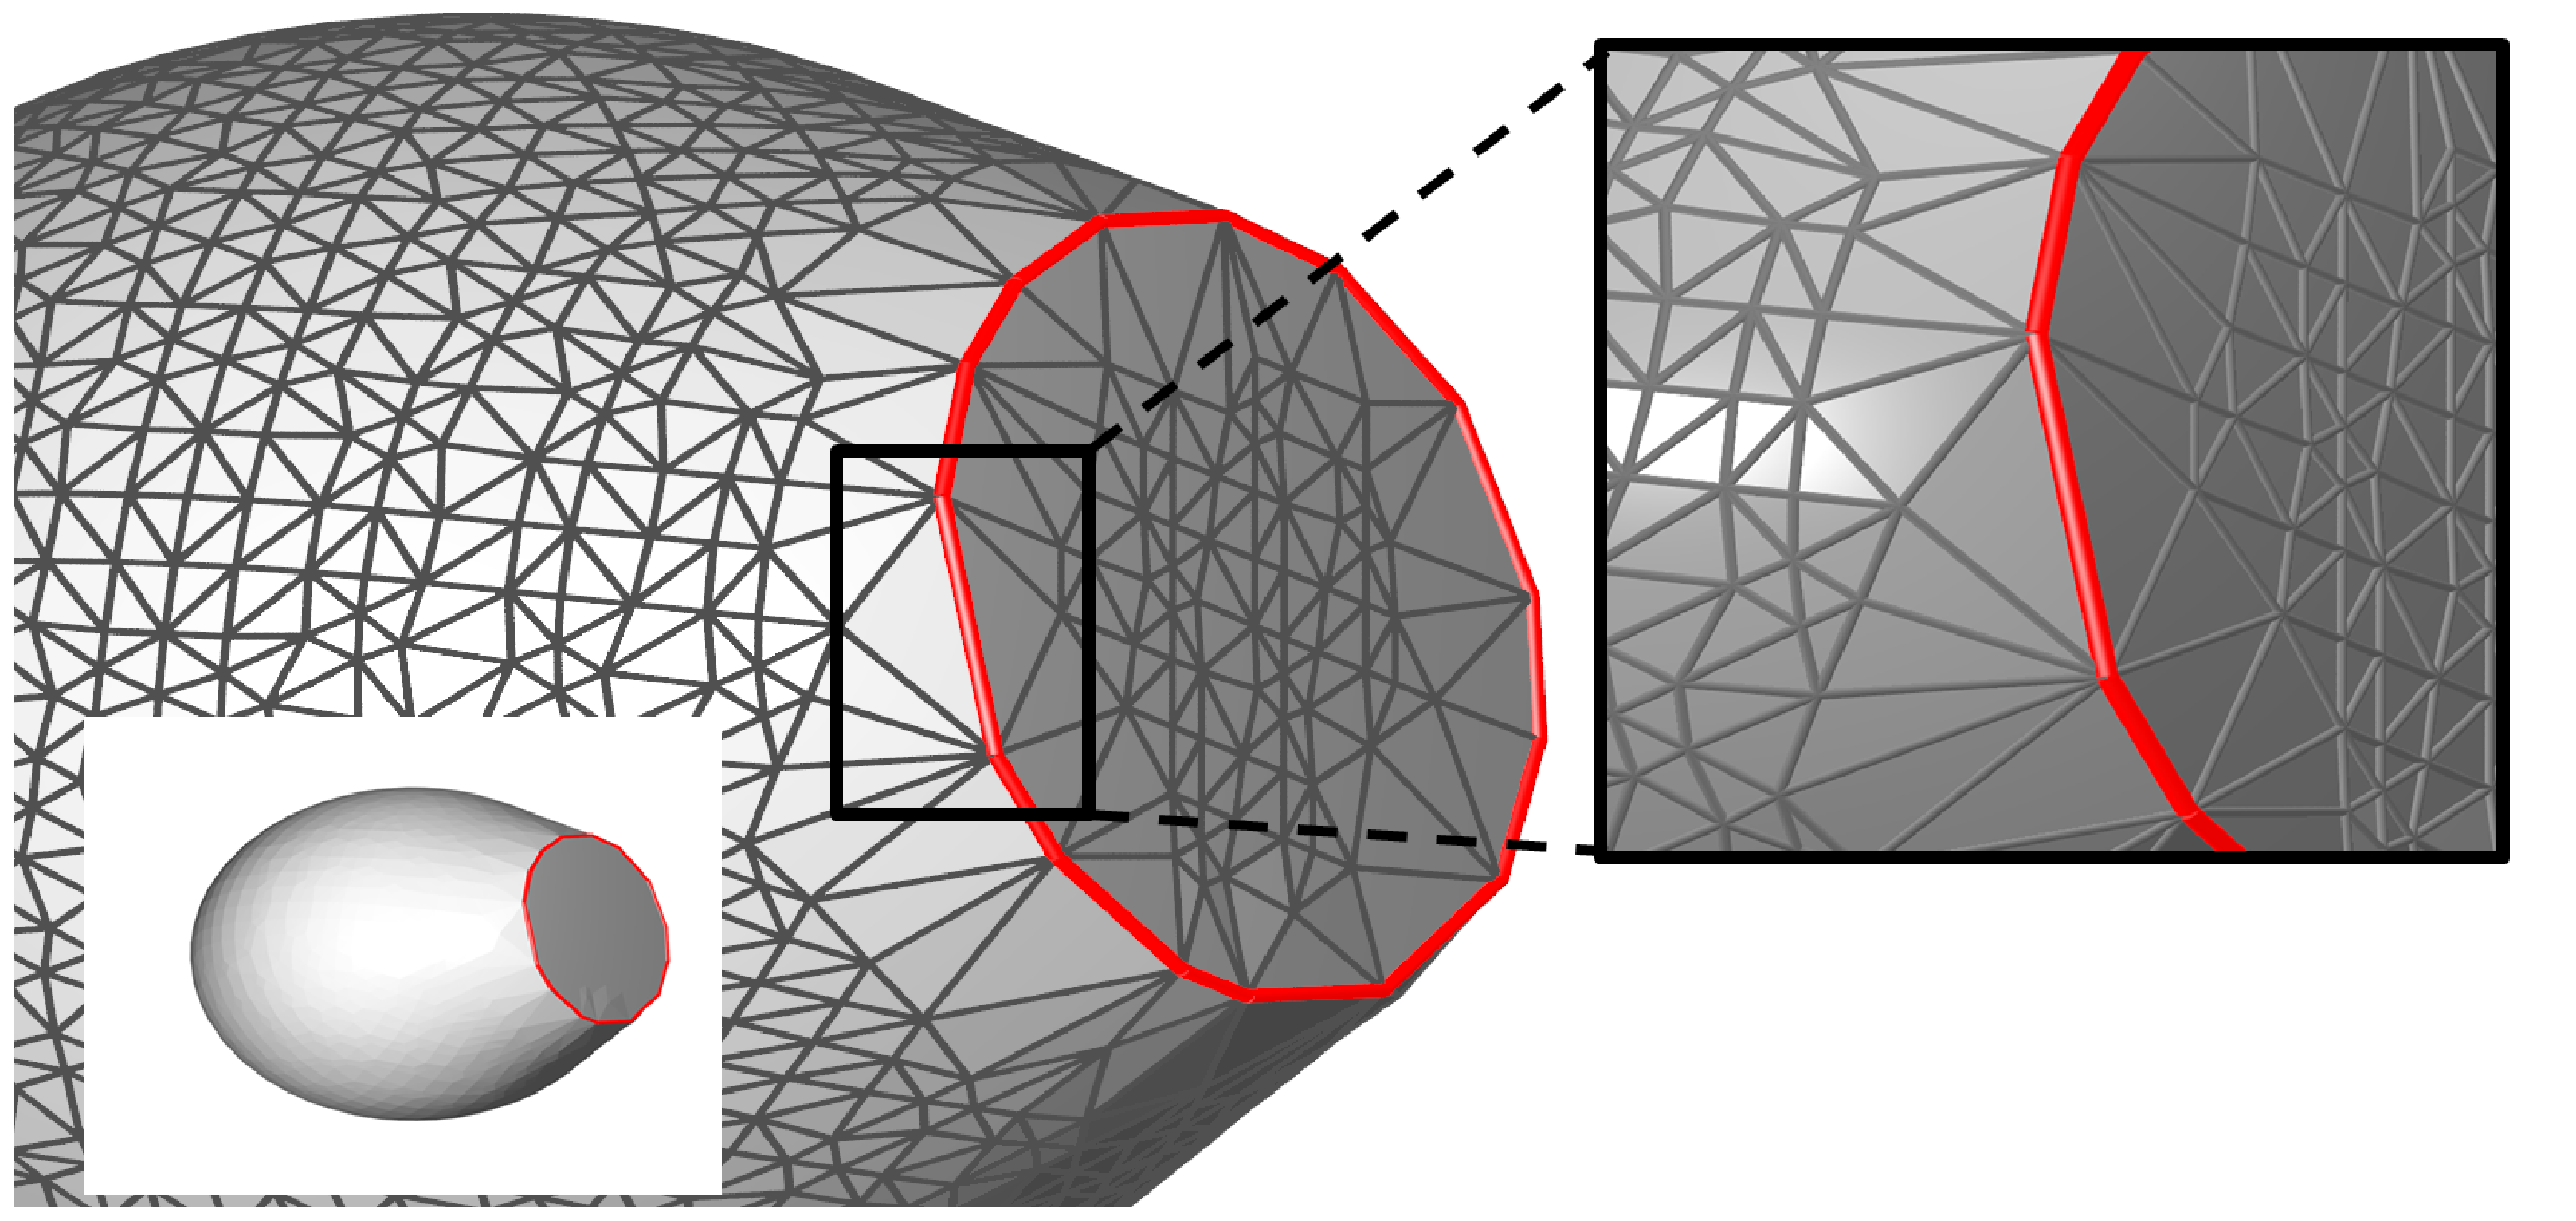
\includegraphics[width=0.5\linewidth]{images/cannon2.eps}\label{fig:cannon:a}}
	\subfloat[]{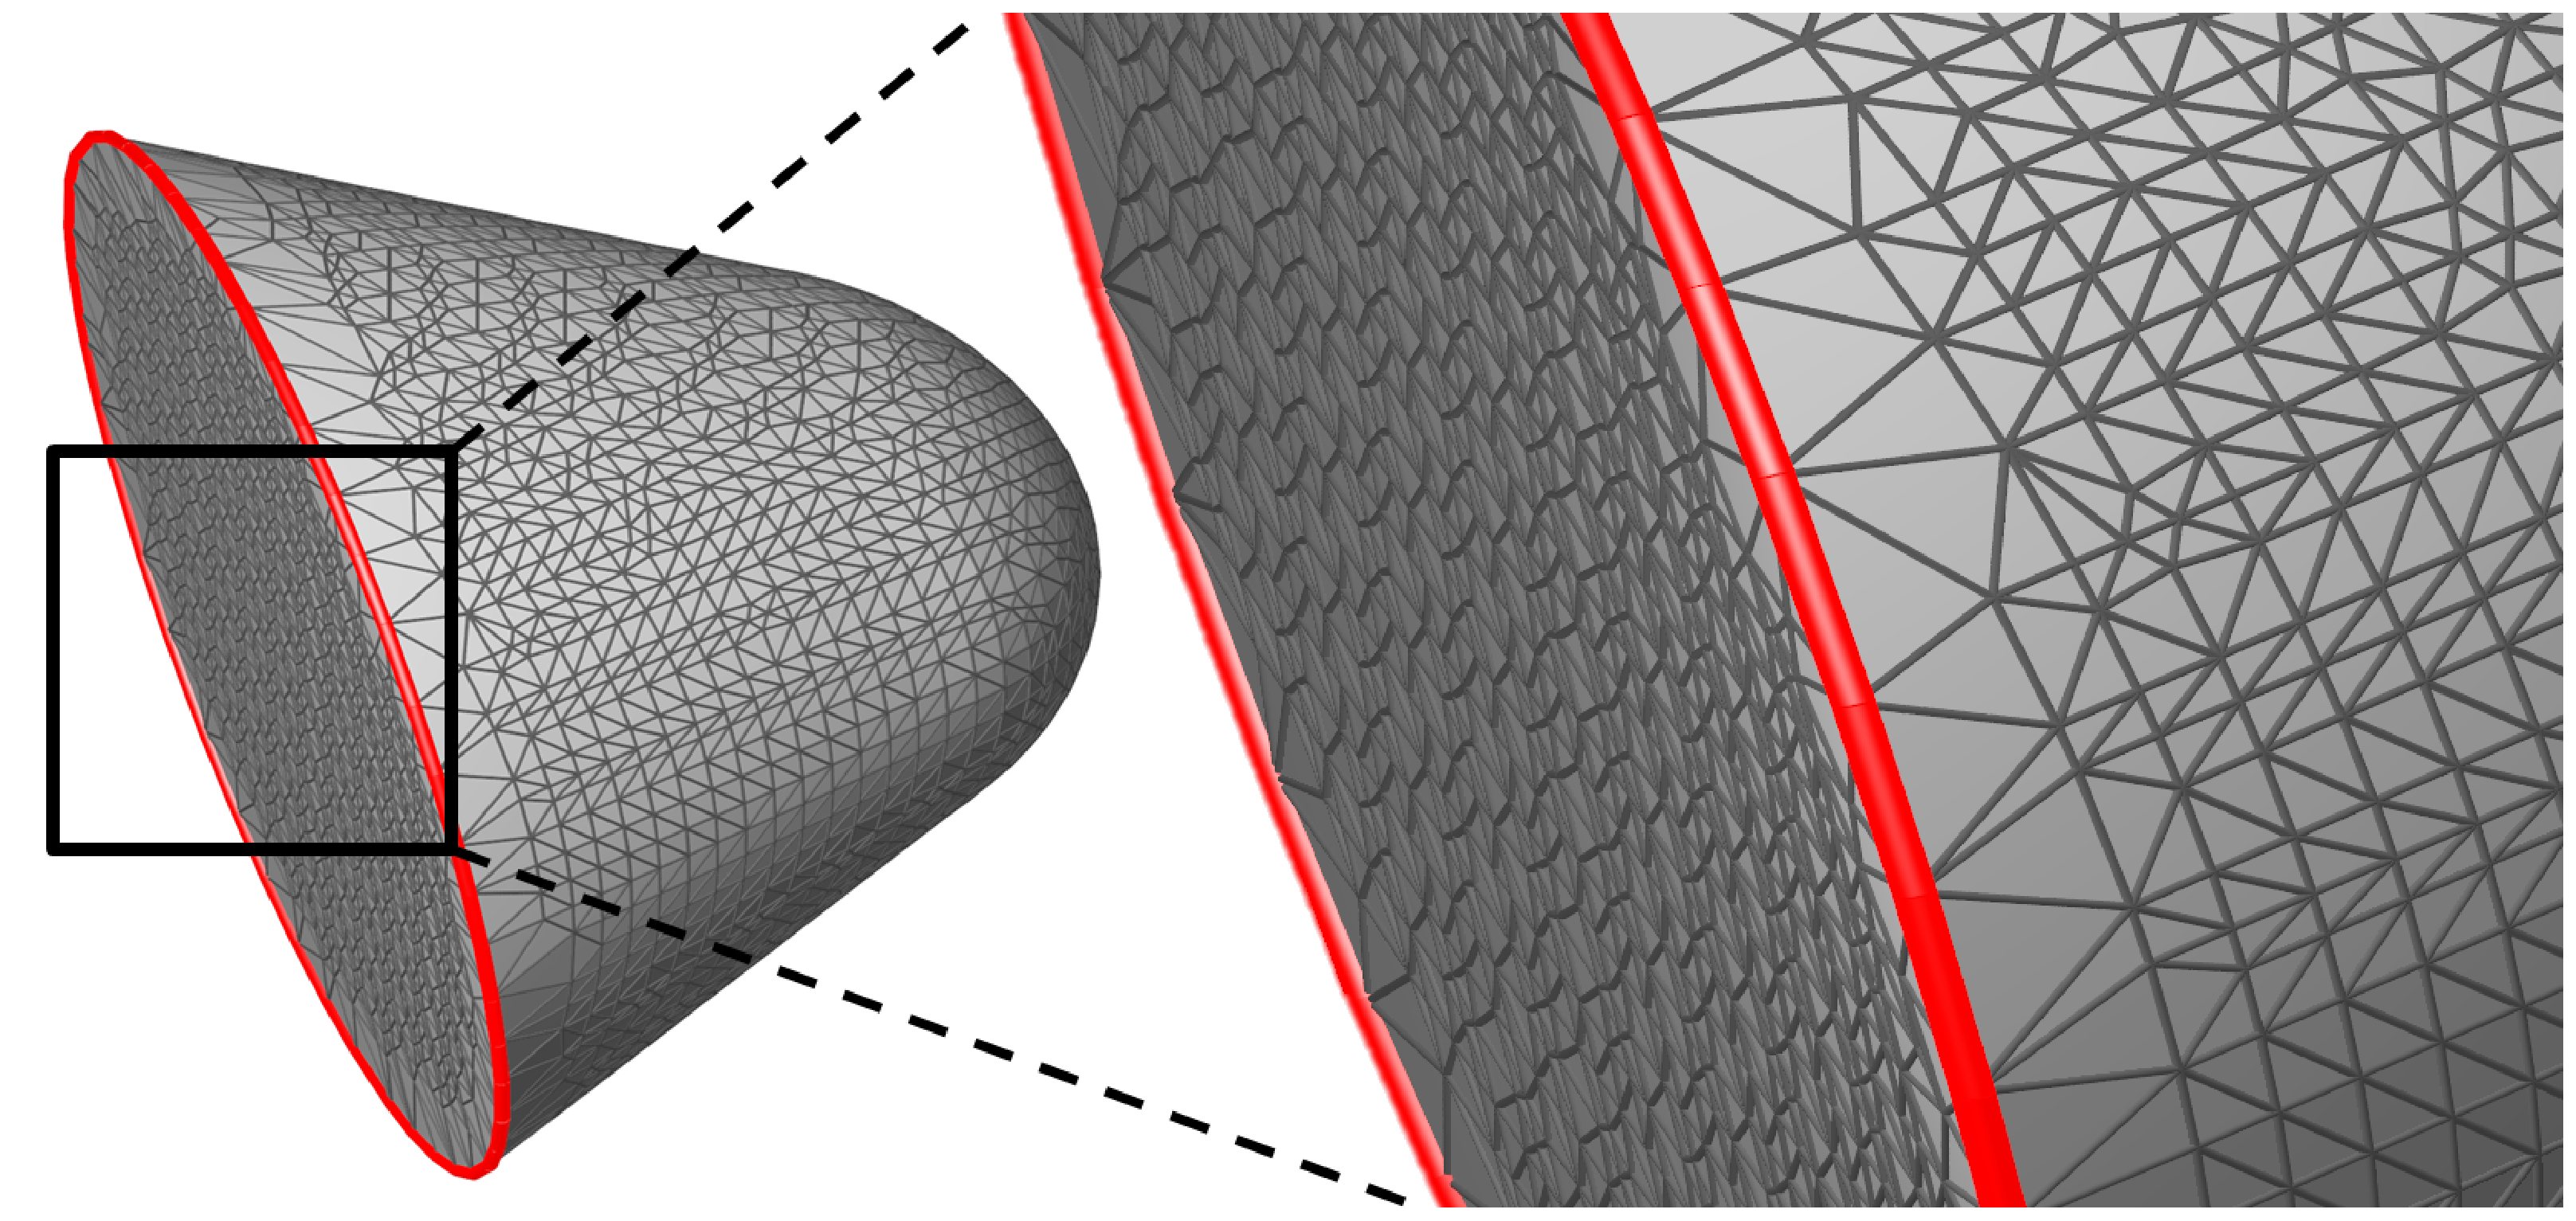
\includegraphics[width=0.5\linewidth]{images/cone2.eps}\label{fig:cone:a}}
	\caption{Result of algorithm SHREC with RELIGRAD gradients on Cannon and Cone datasets}
	\label{fig:cannon_cone}
\end{figure}
\section{Experimental Results on CT Data}
We tested the SHREC algorithm on a number of real industrial dataset. Here we show the results on three of the them. 
Figure~\ref{fig:ict:hondaEng} shows the result of reconstruction on a subset of a Honda Engine data set using SHREC and RELIGRAD. The Honda engine data is $411*431*61$ in dimension. The magnified regions (images with black border) show that the sharp edges are well reconstructed. In yellow border boxes, we see magnified parts of the mesh along with the sharp and non-sharp edges generated by SHREC. In red we see an image of the original part which is reconstructed. 


Figure~\ref{fig:ict:volt} shows the result on our Volt dataset; The dimension of the data set is $101*111*61$. Volt is a scan of a generic 440 voltage electrical connector. Once again we see that SHREC along with RELIGRAD is able to reconstruct the sharp (flange-like) curves accurately. Finally, Figure~\ref{fig:ict:CMM} shows a part of our coordinate measuring machine (CMM) data (size $500*500*196$), Figure~\protect\subref*{fig:ict:CMM:a} shows the reconstruction result. Figure~\protect\subref*{fig:ict:CMM:b} shows a single slice of the CT scan, mapped to the ``heat" color map. 

Through these reconstructions and others we have confirmed that SHREC performs well on real industrial CT data sets. 
\begin{figure}\centering
	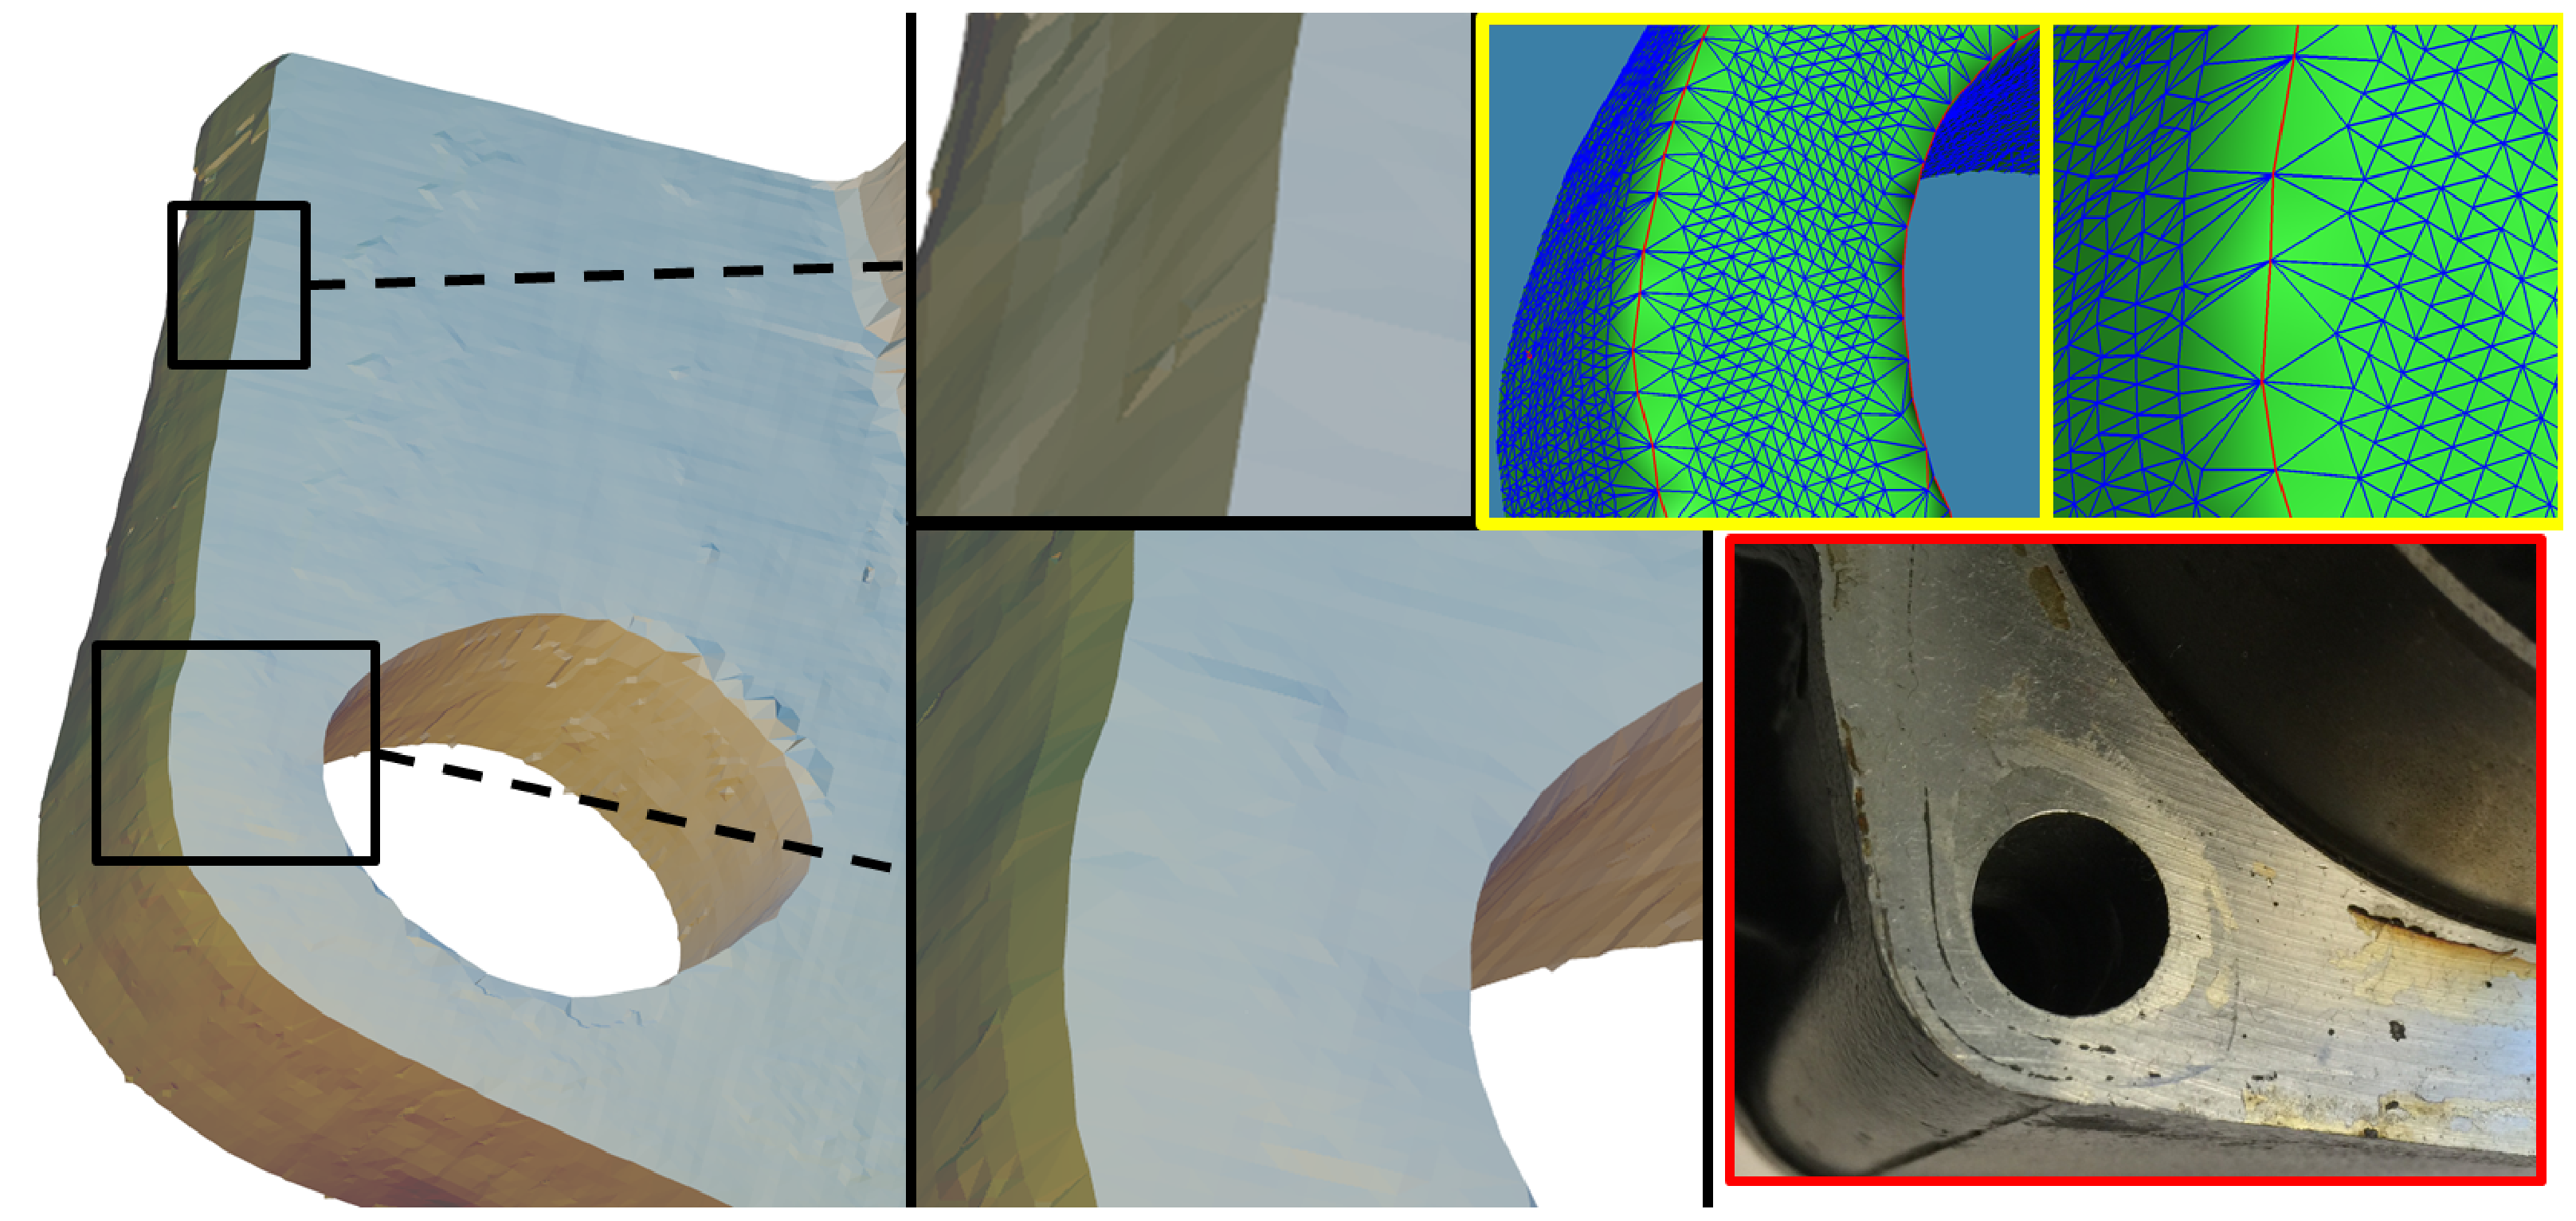
\includegraphics[width=\linewidth]{images/ictsetA_2.eps}
	\caption{SHREC with RELIGRAD gradients computed from part of industrial CT data (Honda Engine). Magnified regions show ``sharp" edges reconstructed. In red, picture from the original item.}
	\label{fig:ict:hondaEng}
\end{figure}
\begin{figure}\centering
	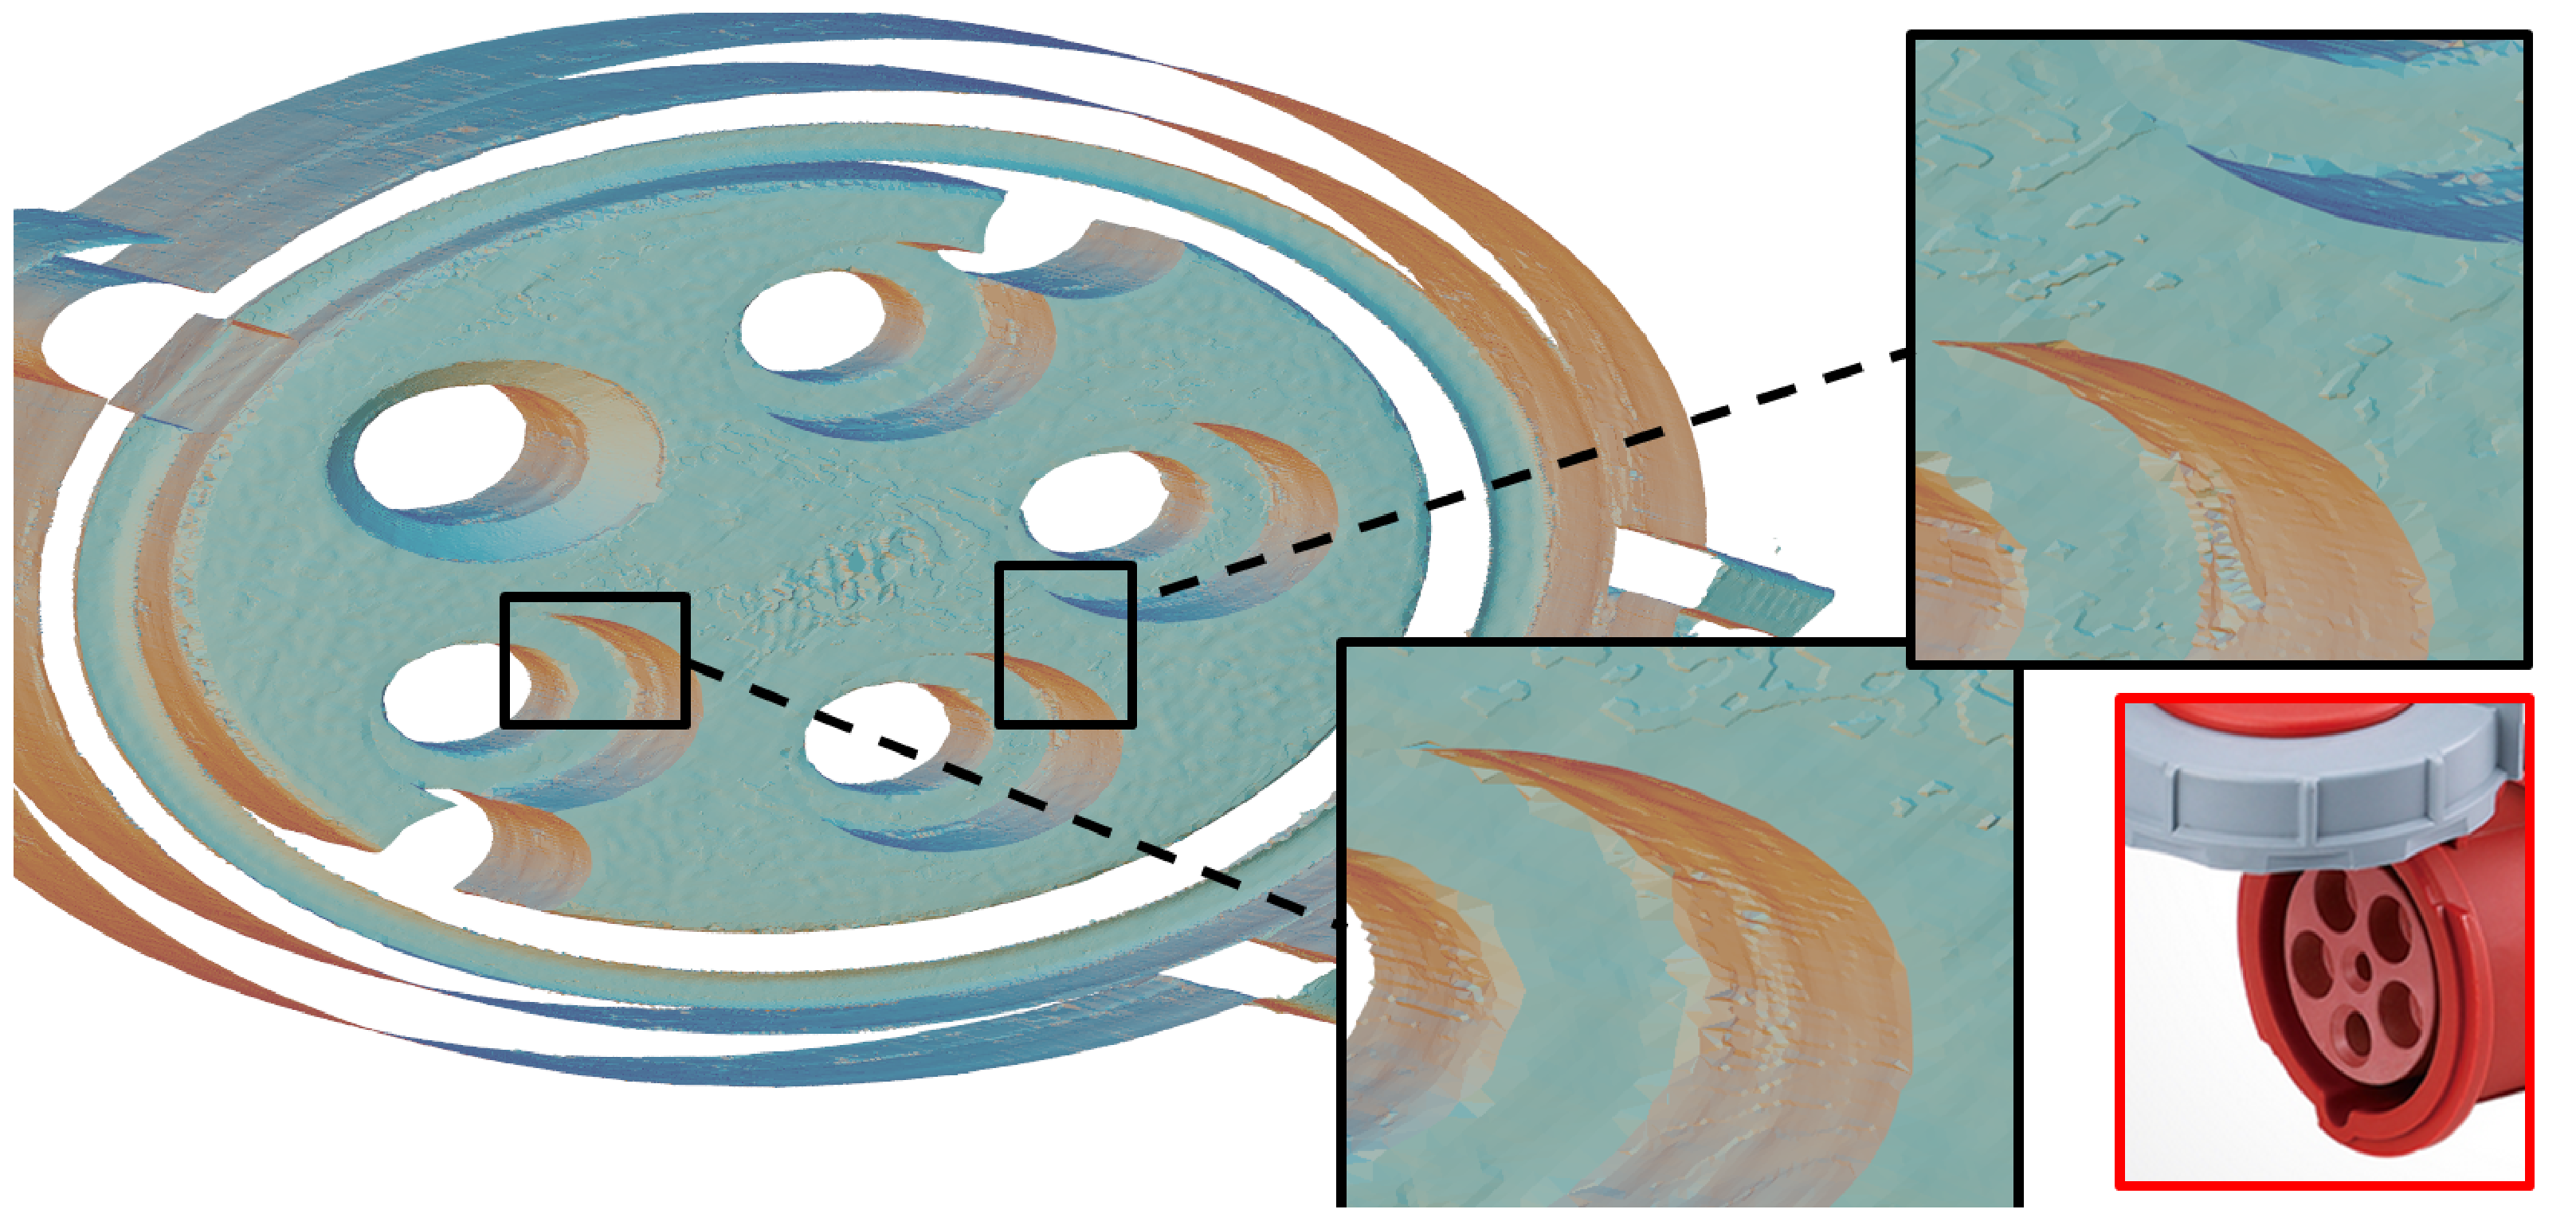
\includegraphics[width=\linewidth]{images/volt.eps}
	\caption{SHREC with RELIGRAD gradients computed from part of the VOLT data. Magnified regions show ``sharp" reconstructed edges. In red picture of the original item.}
	\label{fig:ict:volt}
\end{figure}
\begin{figure}[htb]
	\centering
	\subfloat[]{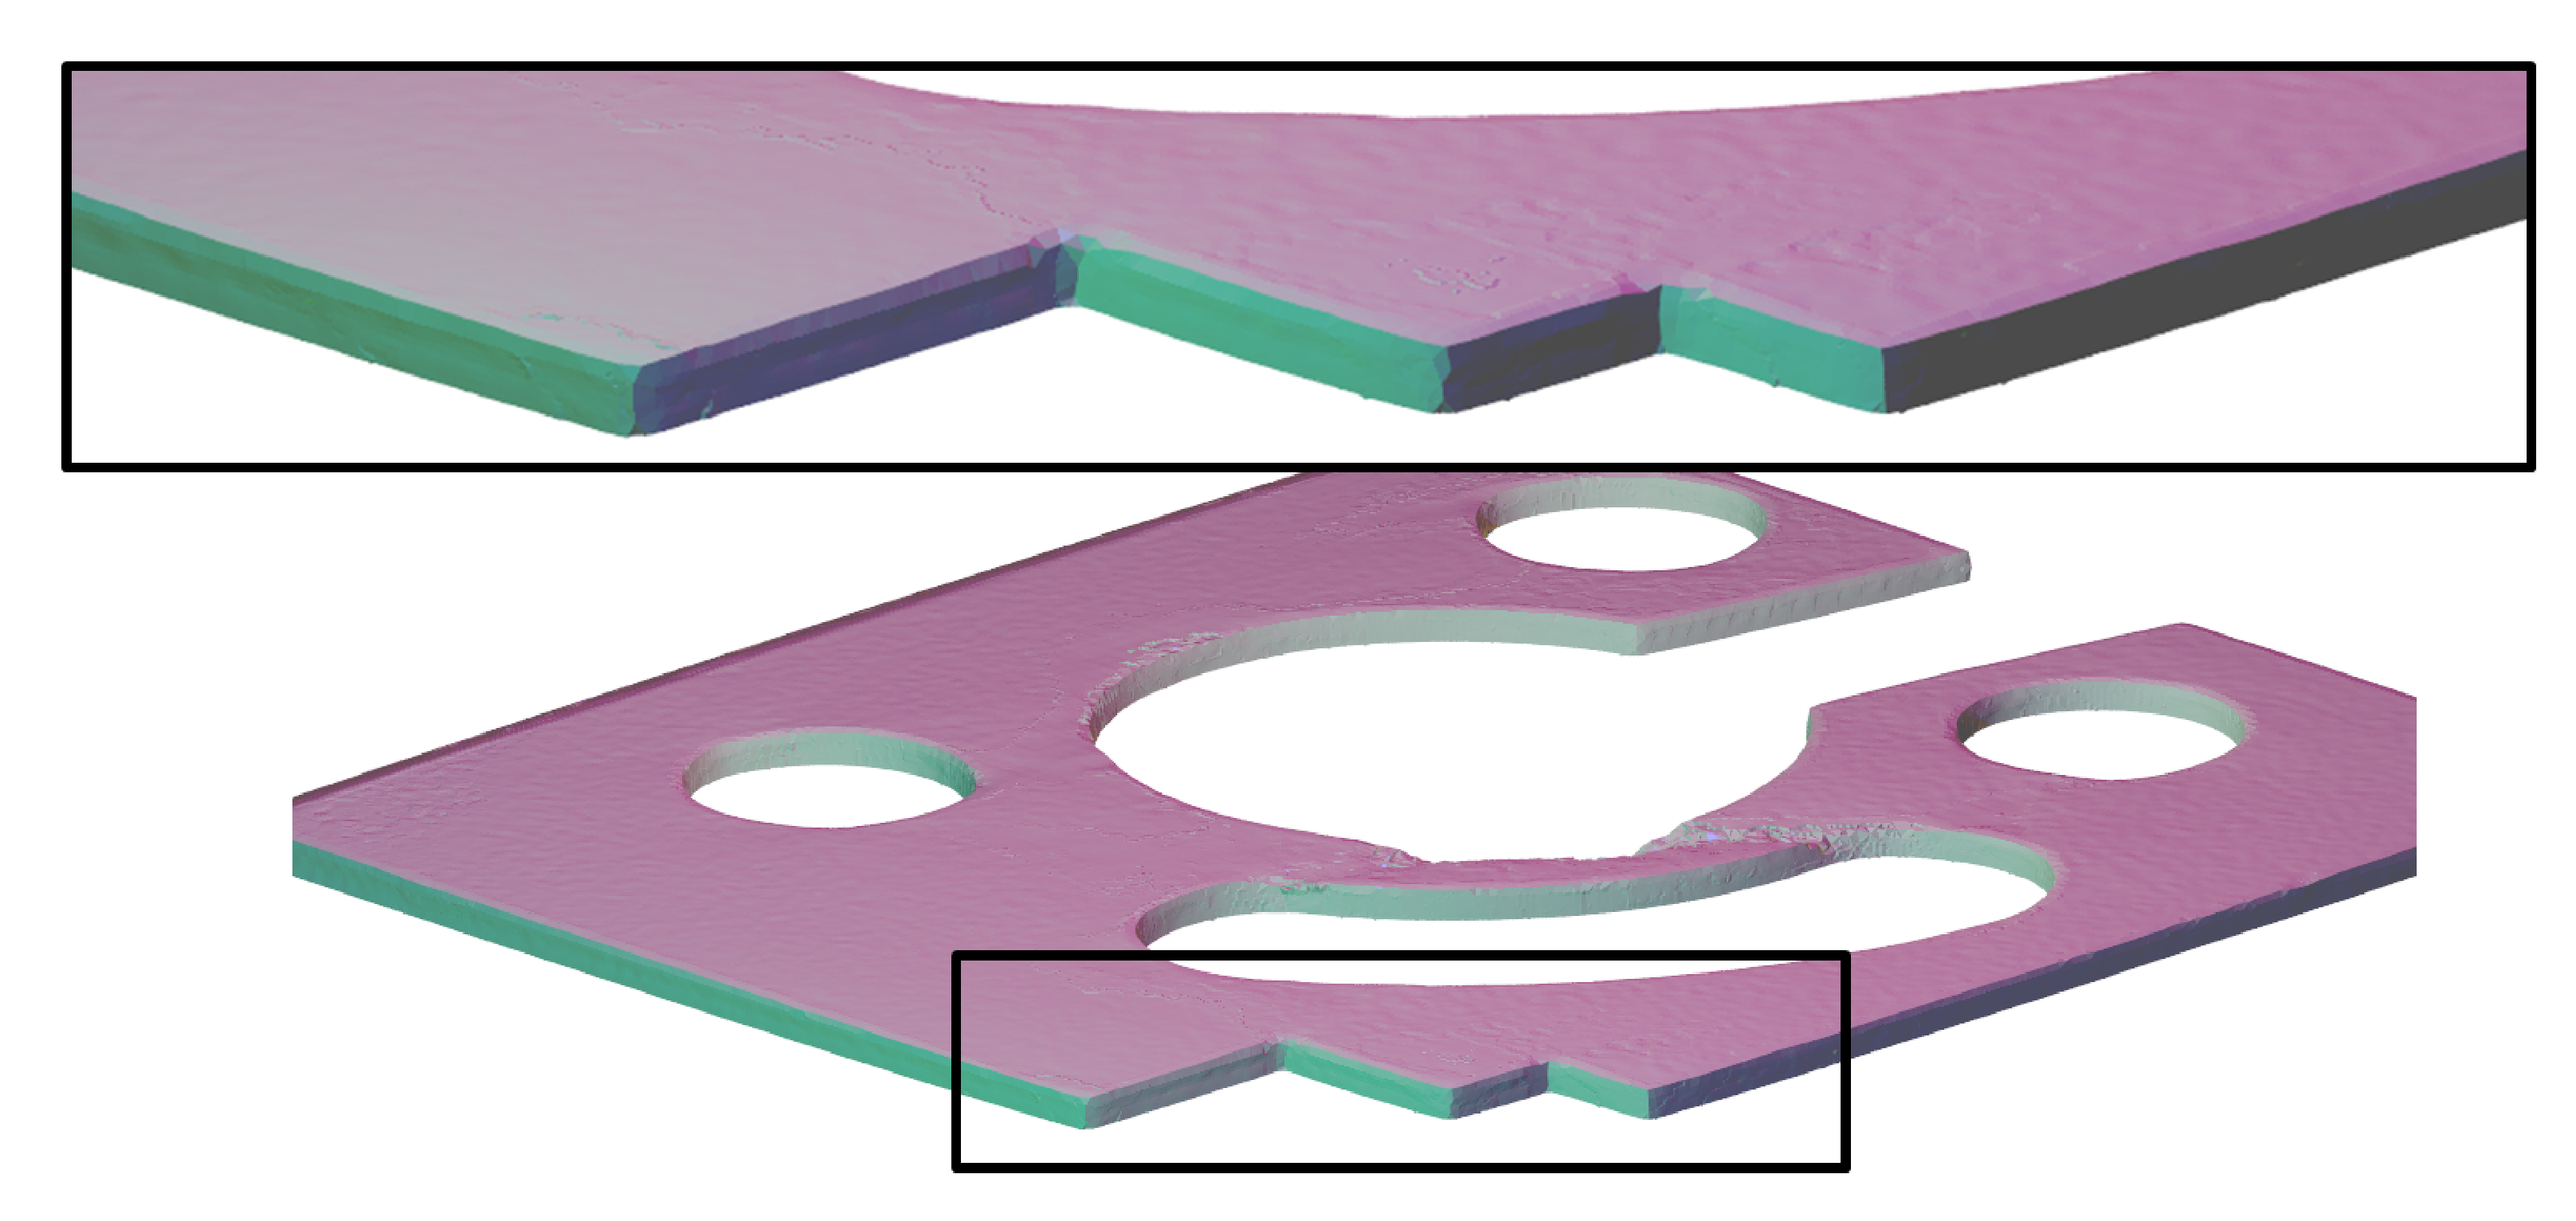
\includegraphics[width=\linewidth]{images/cmm.eps}\label{fig:ict:CMM:a}}\\
	\subfloat[]{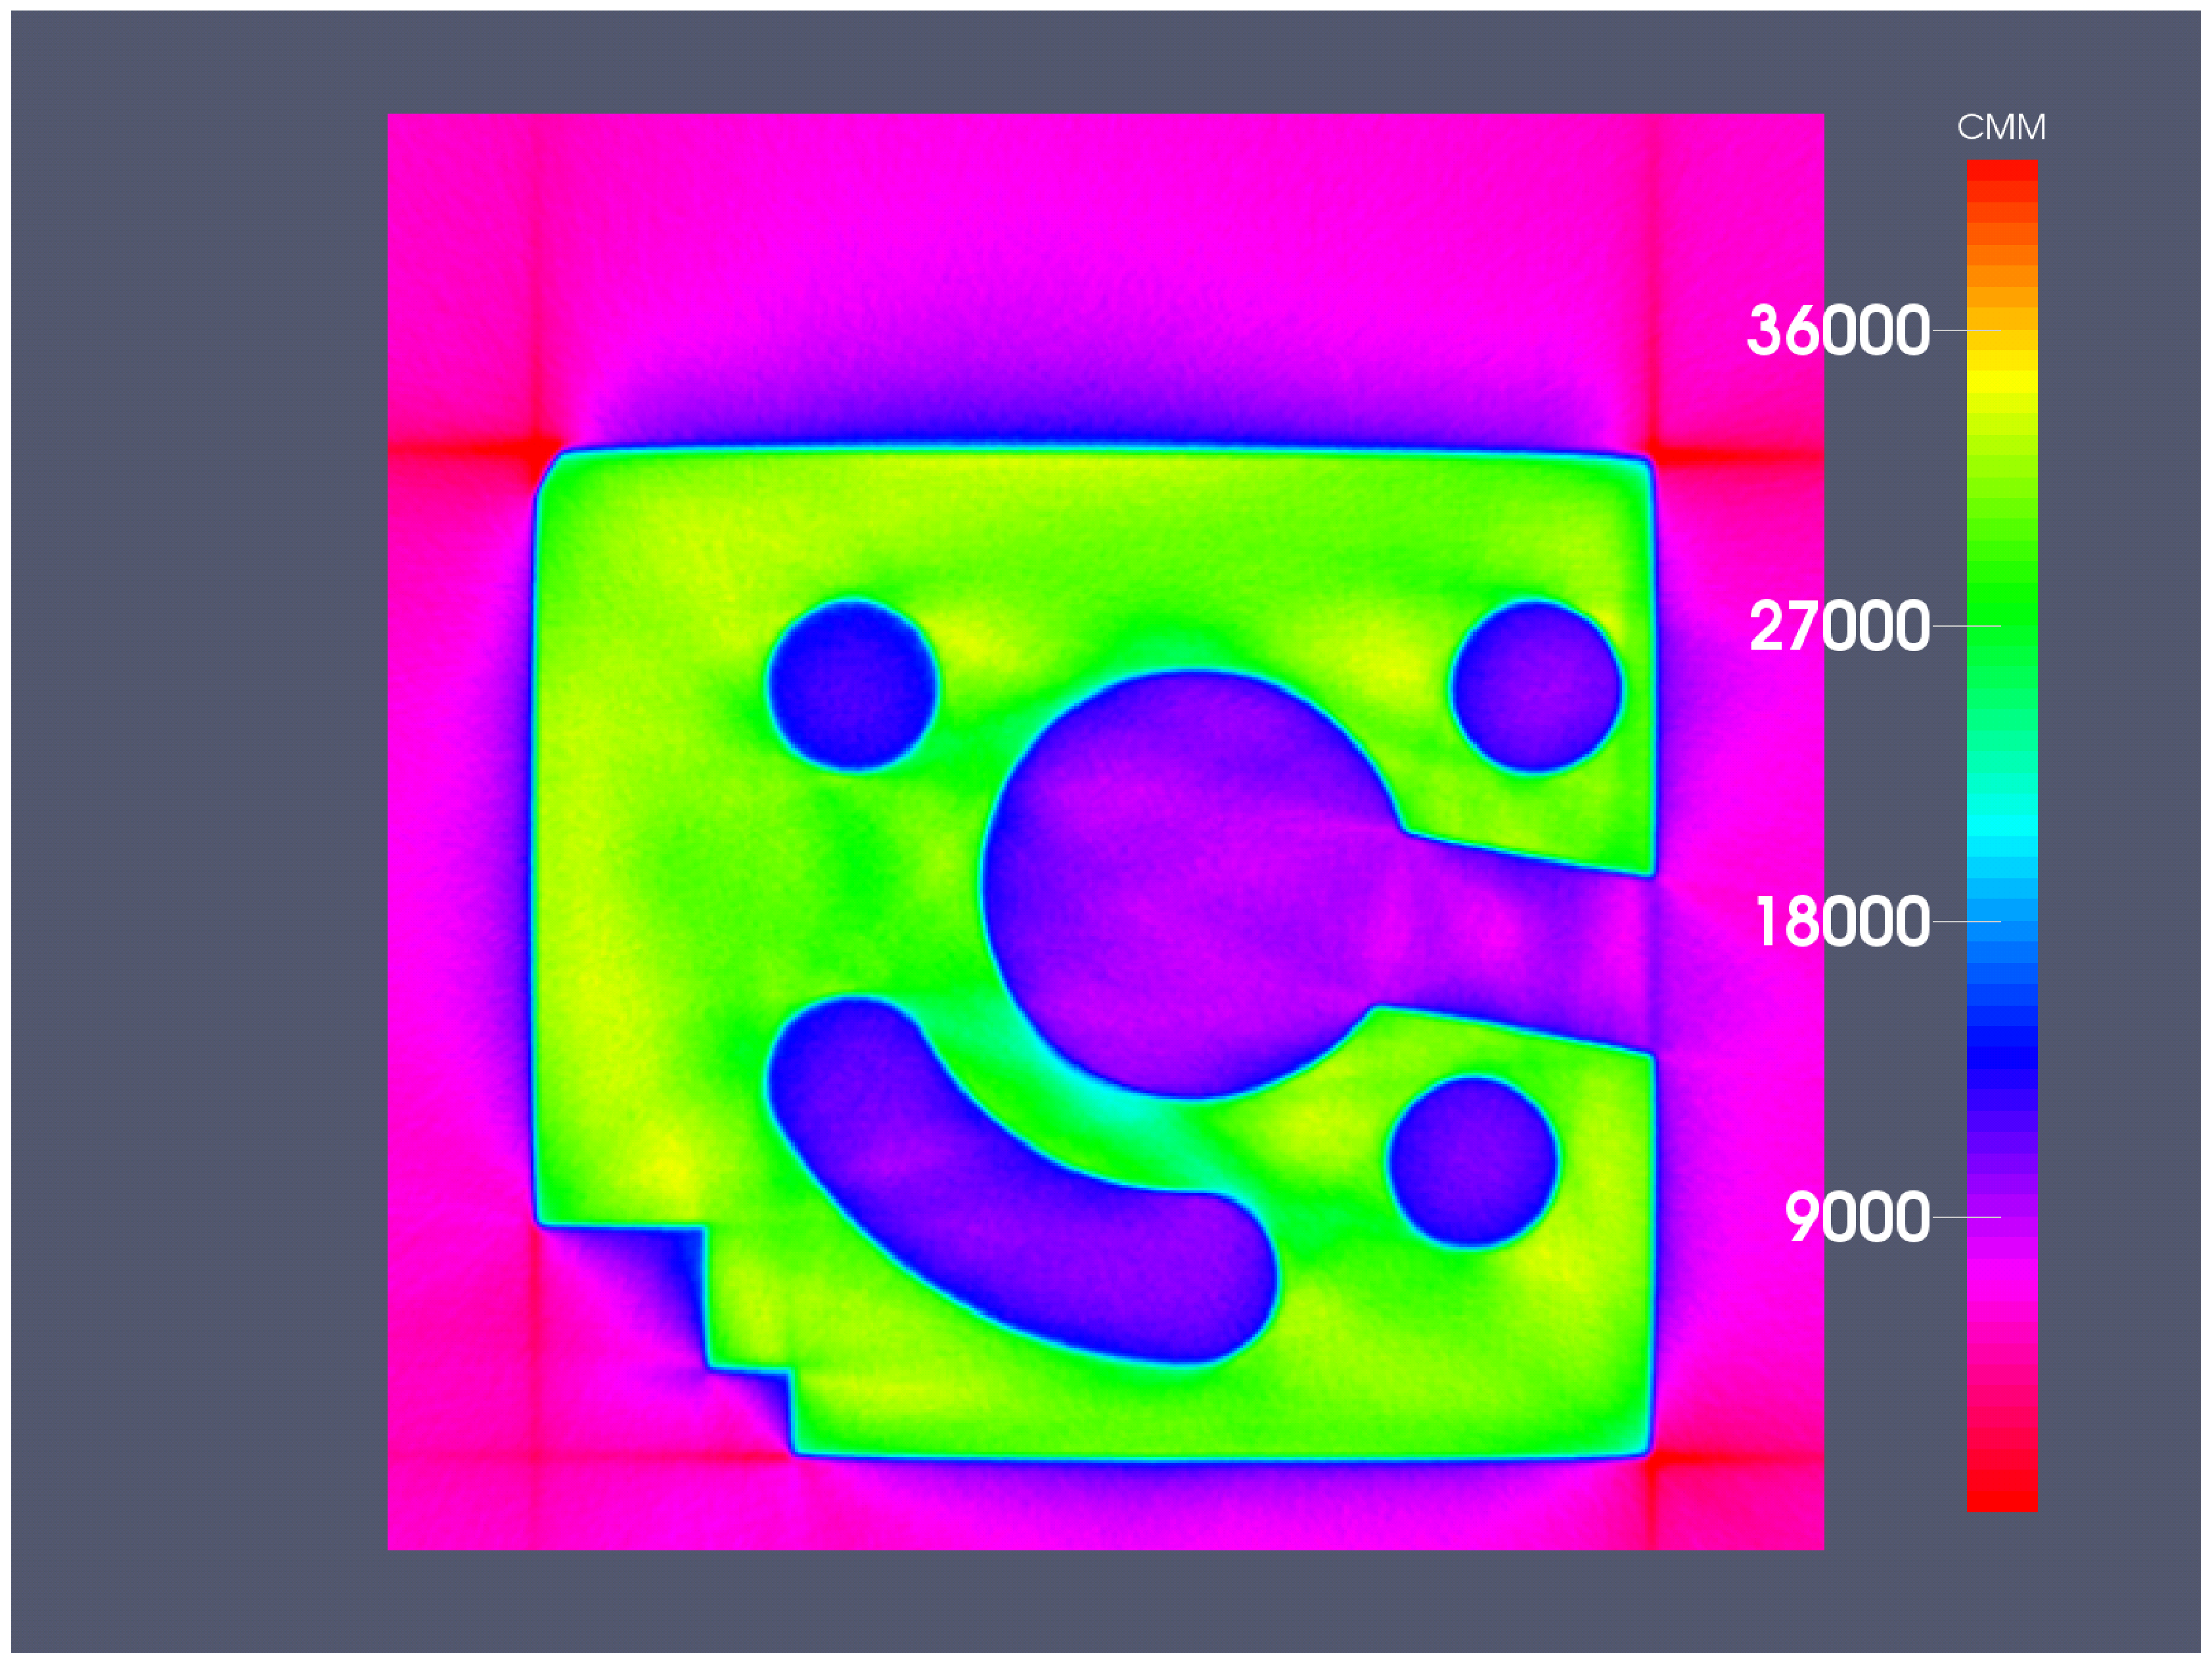
\includegraphics[width=0.5\linewidth]{images/CMM.singleSliceXY.eps}\label{fig:ict:CMM:b}}
	\caption{(a) SHREC with RELIGRAD gradients computed from part of the CMM dataset. Magnified regions show ``sharp" reconstructed edges. (b) Single slice of the CT scan, mapped to the ``heat" color map.}\label{fig:ict:CMM}
\end{figure}
\section{Comparison with Other Algorithms}
\label{section:comparison}
\paragraph{Comparison with MergeSharp}
%#150
\begin{figure}[htb]
	\centering
	\subfloat[]{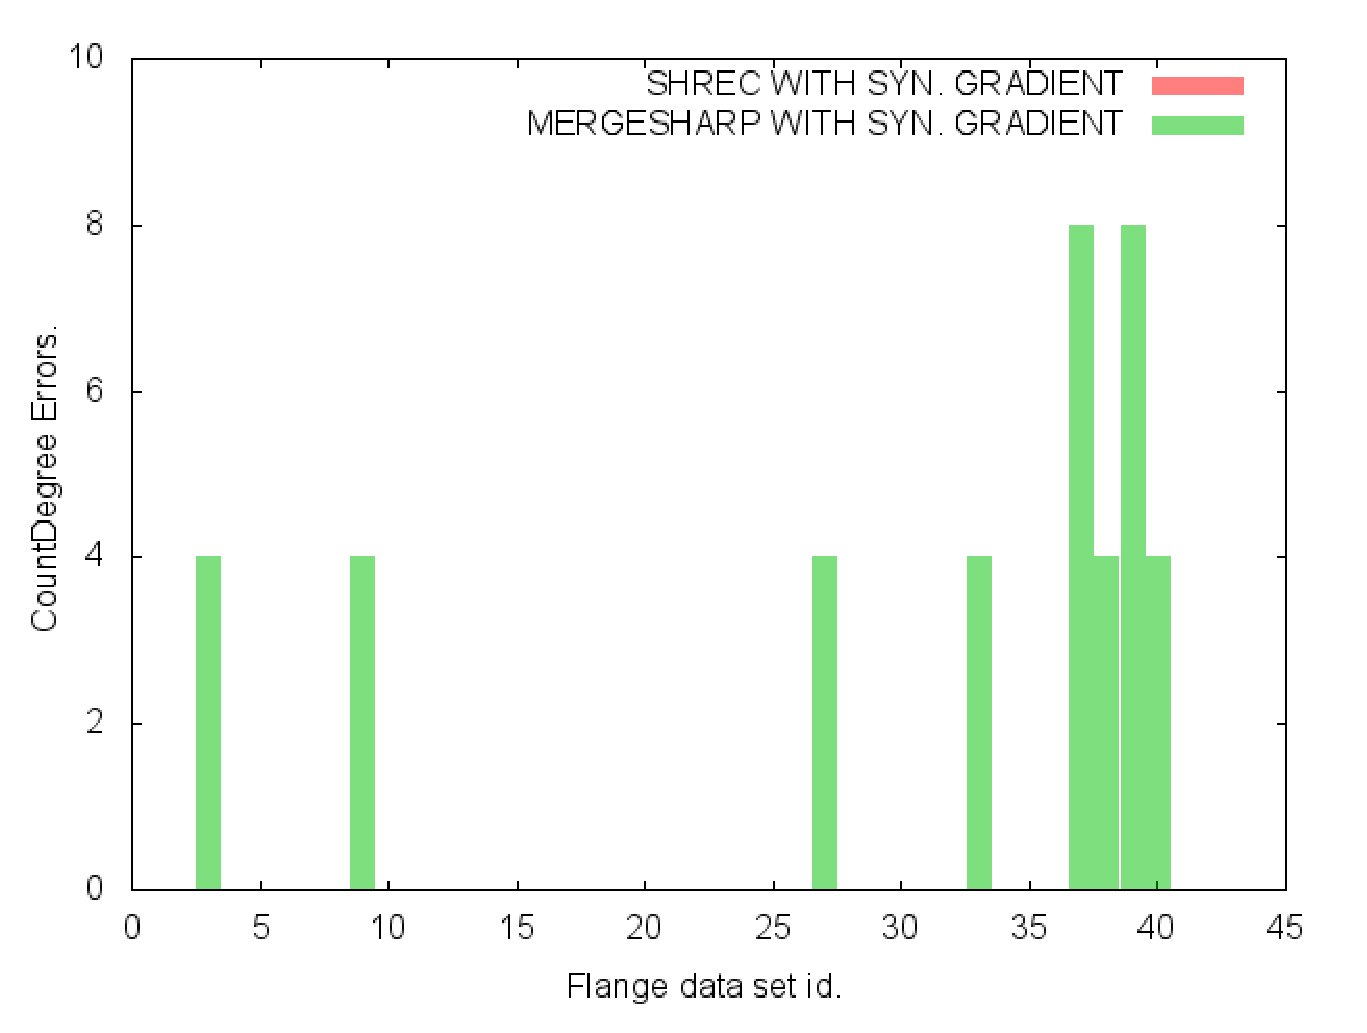
\includegraphics[width=0.8\linewidth]{images/mergeSharpvsShrec.eps}\label{fig:mergesharp:a}}\\
	\subfloat[]{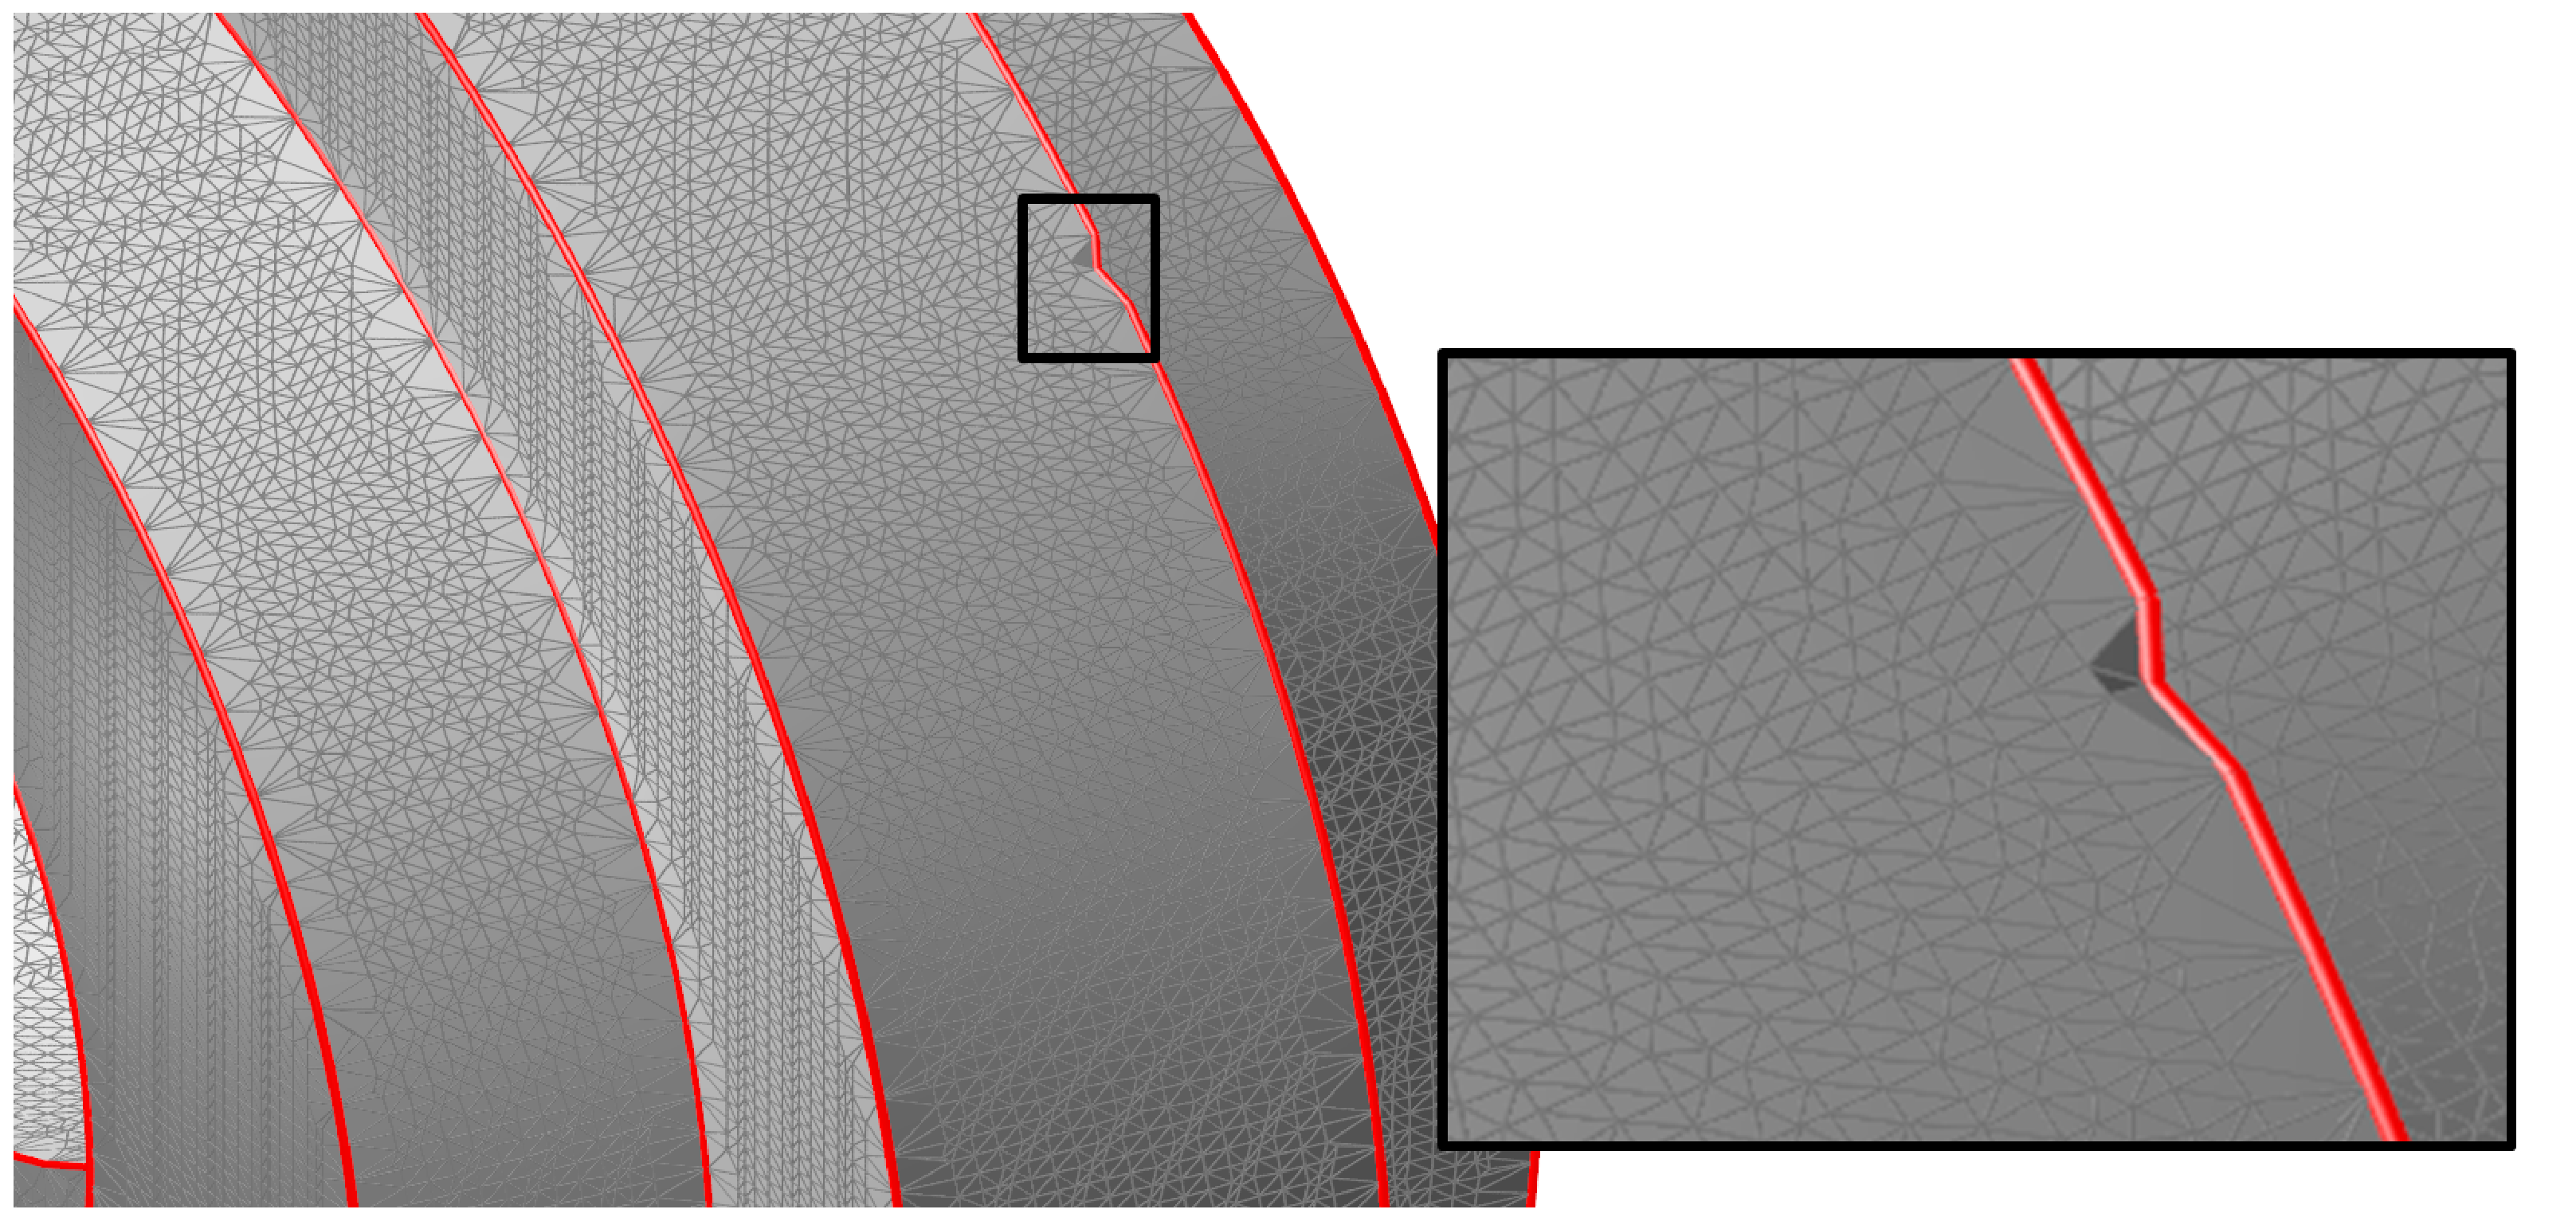
\includegraphics[width=0.6\linewidth]{images/mergeSharpvsShrec2.eps}\label{fig:mergesharp:b}}\\
	\subfloat[]{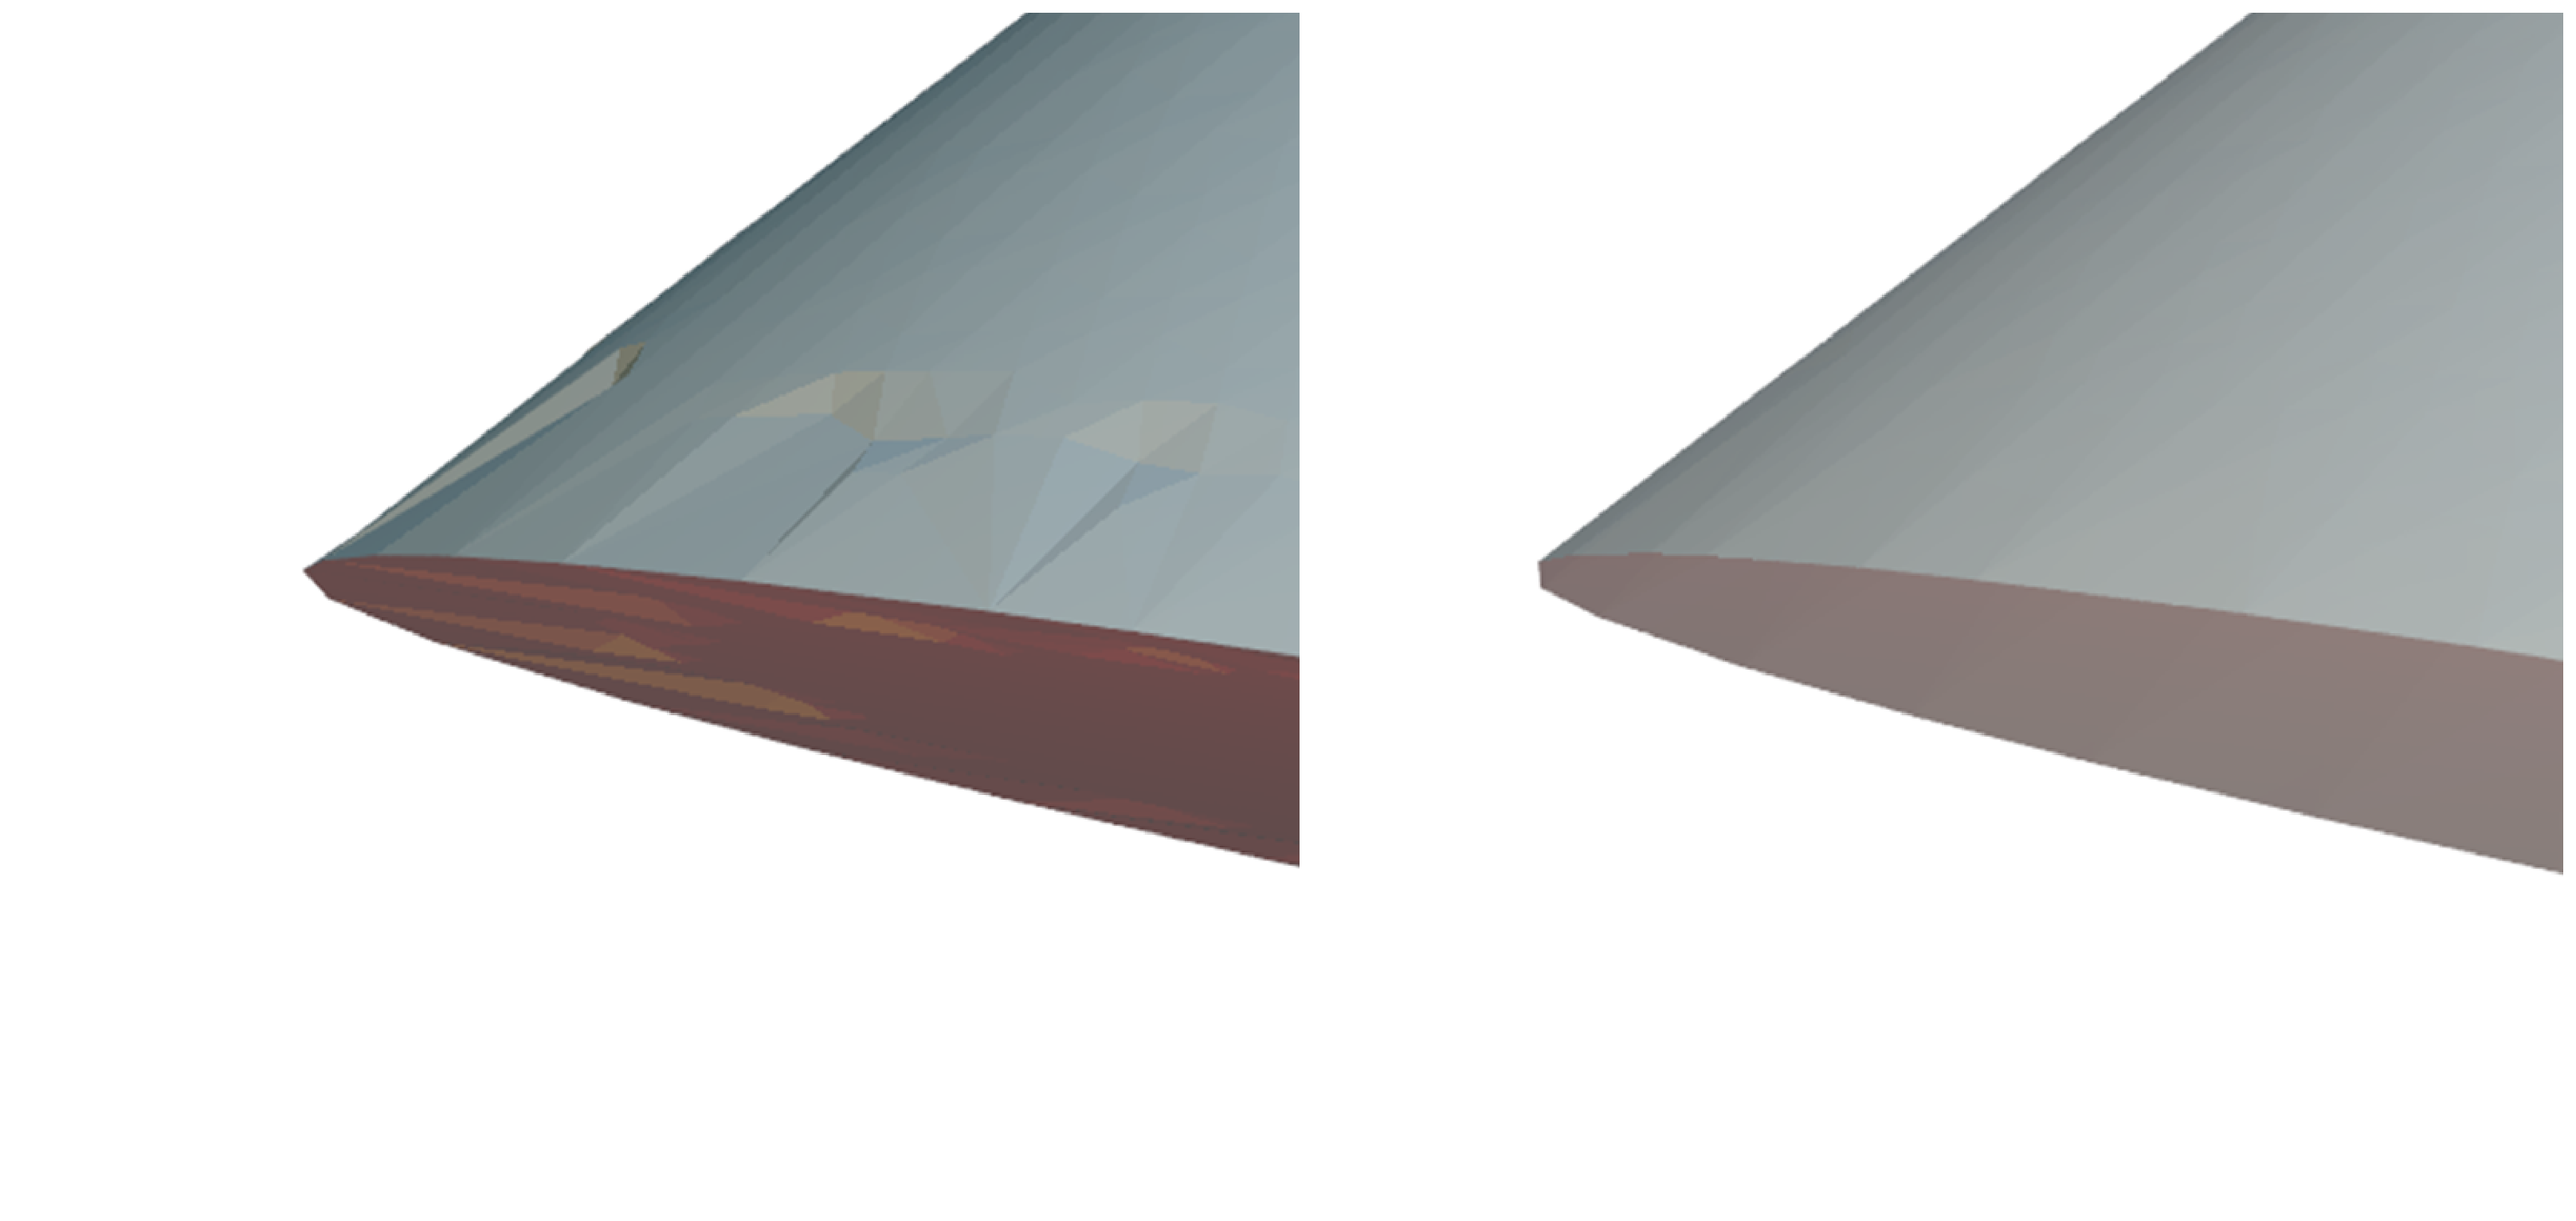
\includegraphics[width=0.6\linewidth]{images/cone_mergesharp.eps}\label{fig:mergesharp:c}}
	\caption{Result of  MERGESHARP and SHREC with synthetic gradients. (a) Summary results of  CountDegree errors of 40 Flange datasets. SHREC does not produce an errors. (b) Result on one particular data set using MERGESHARP, magnified region shows one of the ``notches" created. (c) Apart from ``Notches", MERGESHARP produces gentle dimples which decays the visual quality. Magnified region shows a portion of a Cone dataset (Left) MERGESHARP (Right) SHREC. }
	\label{fig:mergeSharpVShrec}
\end{figure}	
We first compare our algorithm with MERGESHARP ~\cite{bw-cisec-13}, MERGESHARP uses synthetic gradients. Figure~\protect\subref*{fig:mergesharp:a} shows the summary of CountDegree results of running MERGESHARP on 40 Flange datasets using synthetic gradients. SHREC as discussed above does not generate any errors with synthetic gradients. Figure~\protect\subref*{fig:mergesharp:b} shows the result on one of the Flange data sets. MERGESHARP produces ``notches" such as the one shown in Figure~\protect\subref*{fig:mergesharp:b}.

MERGESHARP also produces gentle dimples such as the ones in the edge of a Cone data set shown in Figure~\protect\subref*{fig:mergesharp:c}, SHREC does not produce them. 	
\paragraph{Comparison with Cocone}
We compare our algorithm to the algorithm WeightCocone by Dey et al.~\cite{Dey2012}. WeightCocone reconstructs a surface with sharp edges and corners from a sampled point cloud. WeightCocone takes two inputs; one contains the point cloud, another is a weighted sampling of feature curves. Weight of the sampling will be used as weight of the protecting balls. WeightCocone generates as output a feature sensitive mesh. 

The feature curve (second input to WeightCocone) is constructed using the algorithm FeatureRecon by Dey et al.~\cite{Dey2013}. FeatureRecon extracts feature curves of a surface. The input is a point cloud sampled on the surface. FeatureRecon has two steps, feature point detection and feature curves reconstruction. 
\paragraph{Experimental details:} The input to FeatureRecon is a point cloud. We tested two different input point cloud;
\begin{enumerate}
	\item We applied Marching Cubes~\cite{lc-mchr3-87} on our datasets Sec.\ref{sec:synData}. The vertices of the mesh generated by the Marching Cubes algorithm are then super-sampled using the Monte Carlo point sampling, to generate a point cloud with approximately sixty-five thousand points.
	\item We super-sampled the synthetic meshes Sec.\ref{sec:synData}, to generate generate a point cloud with approximately sixty-five thousand points.
\end{enumerate}
The two different point clouds are used as input to FeatureRecon to extract the feature curves. 
FeatureRecon has nine separate parameters. Experimentally and also noted by the authors Dey et al.~\cite{Dey2013}, we found FeatureRecon to be heavily reliant on parameter fine tuning. We used the following parameter values for our TwoCube datasets, (as suggest by the authors Dey et al.~\cite{Dey2013}). 
$-t = 25,-fl = 0.04, -cl = 0.06, -dc = 0, -\rho3 = 0.32, -\rho1 = 0.0, -rc = 3$.

The feature curves generated using FeatureRecon along with the super-sampled point cloud is used as input to WeighCocone. For comparison test, we compare the known synthetic mesh with the output of WeightCocone. 
We report the degree count of the ``sharp" edges (dihedral angle less than $140^\circ$). We also report the surface angle distances between the output and the synthetic mesh. 
\begin{figure}[t] 
	%dataset t110 reconstructed from perfect mesh 
	\centering 
	\subfloat[]{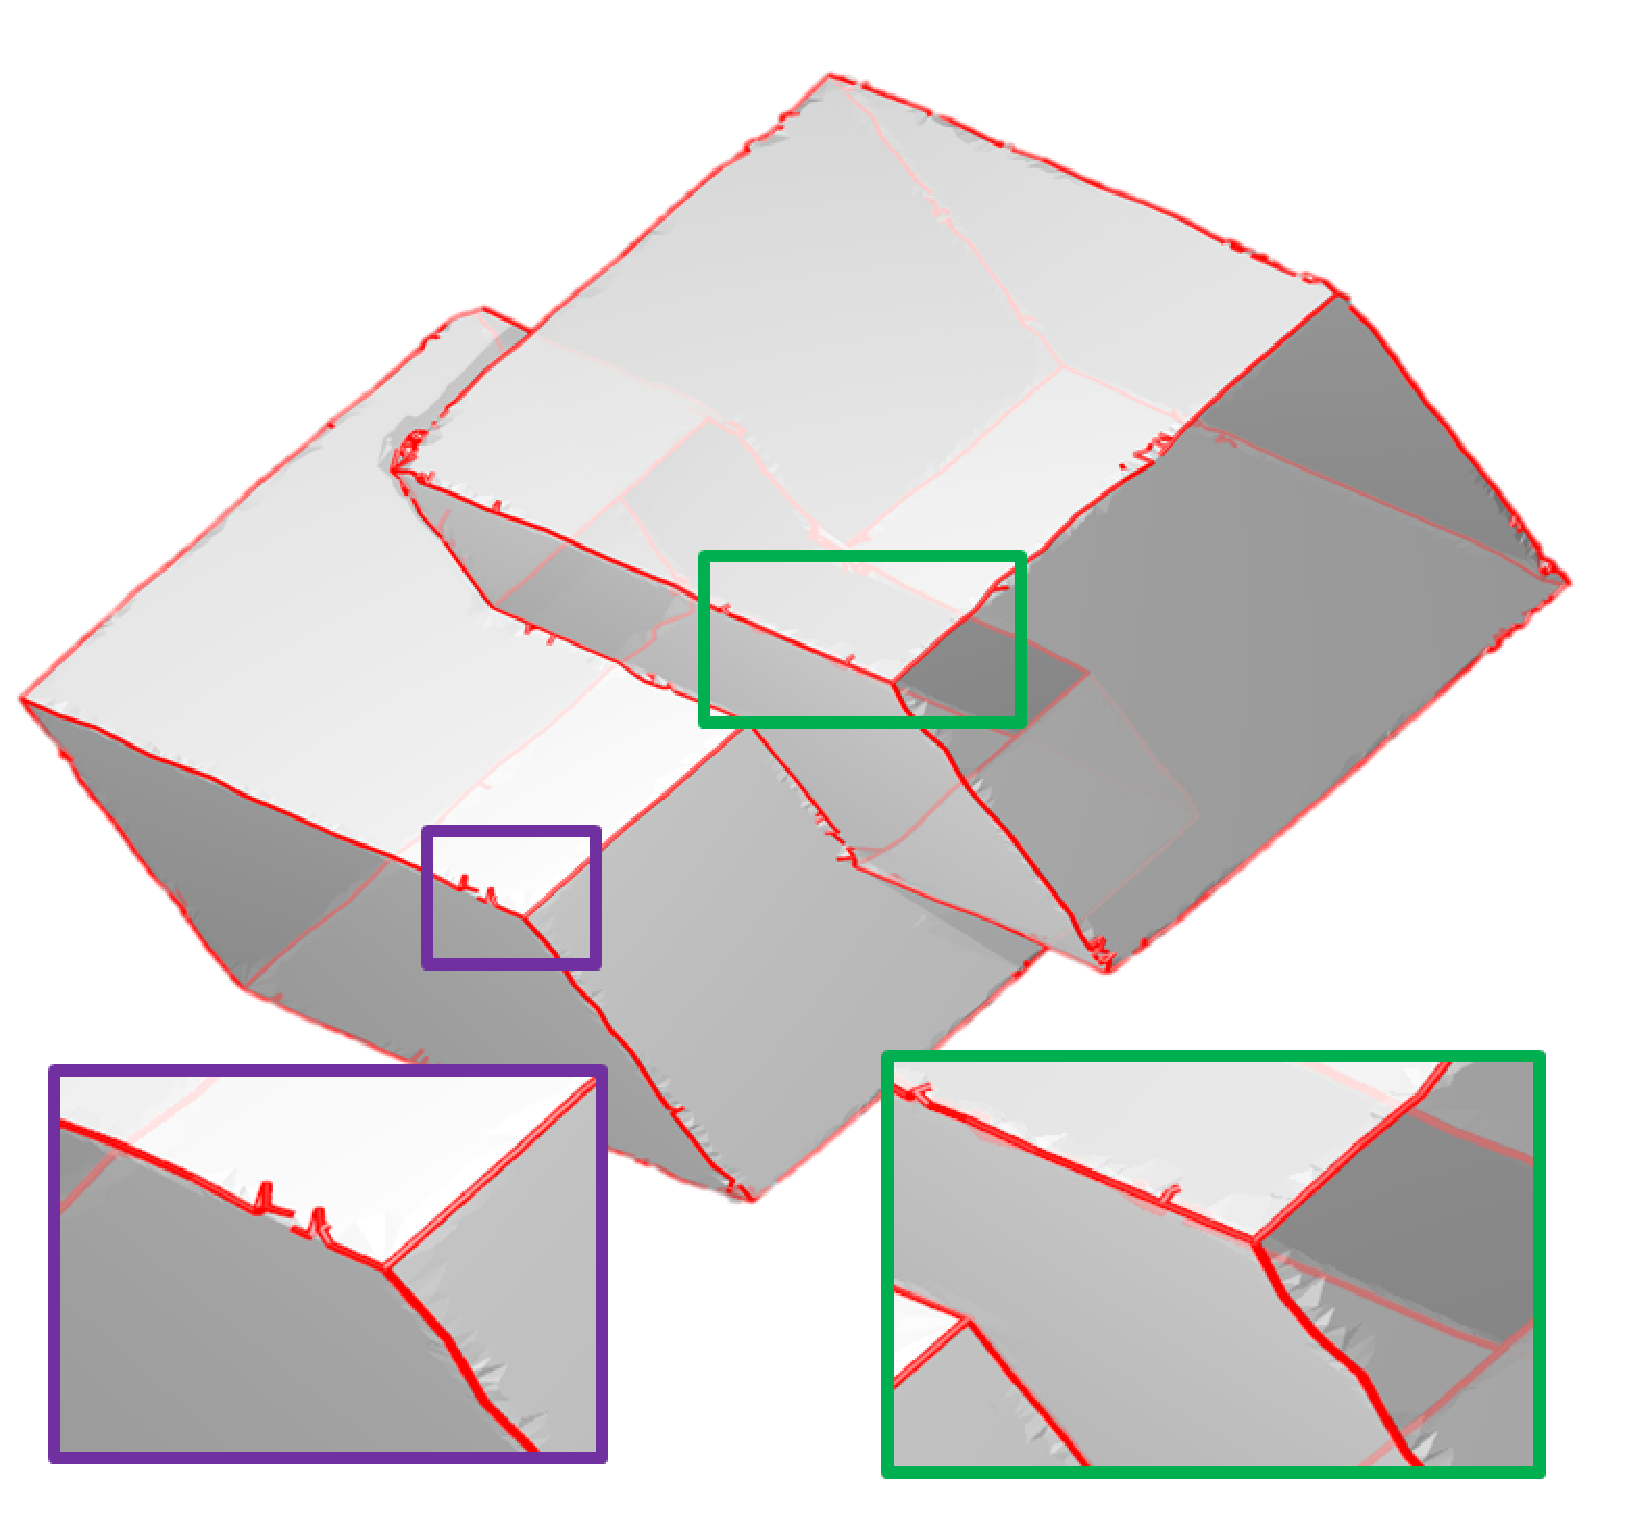
\includegraphics[width=0.5\linewidth]{images/compare_cocone_perfect_mc_a.eps}\label{fig:cocone_img:a}}
		\subfloat[]{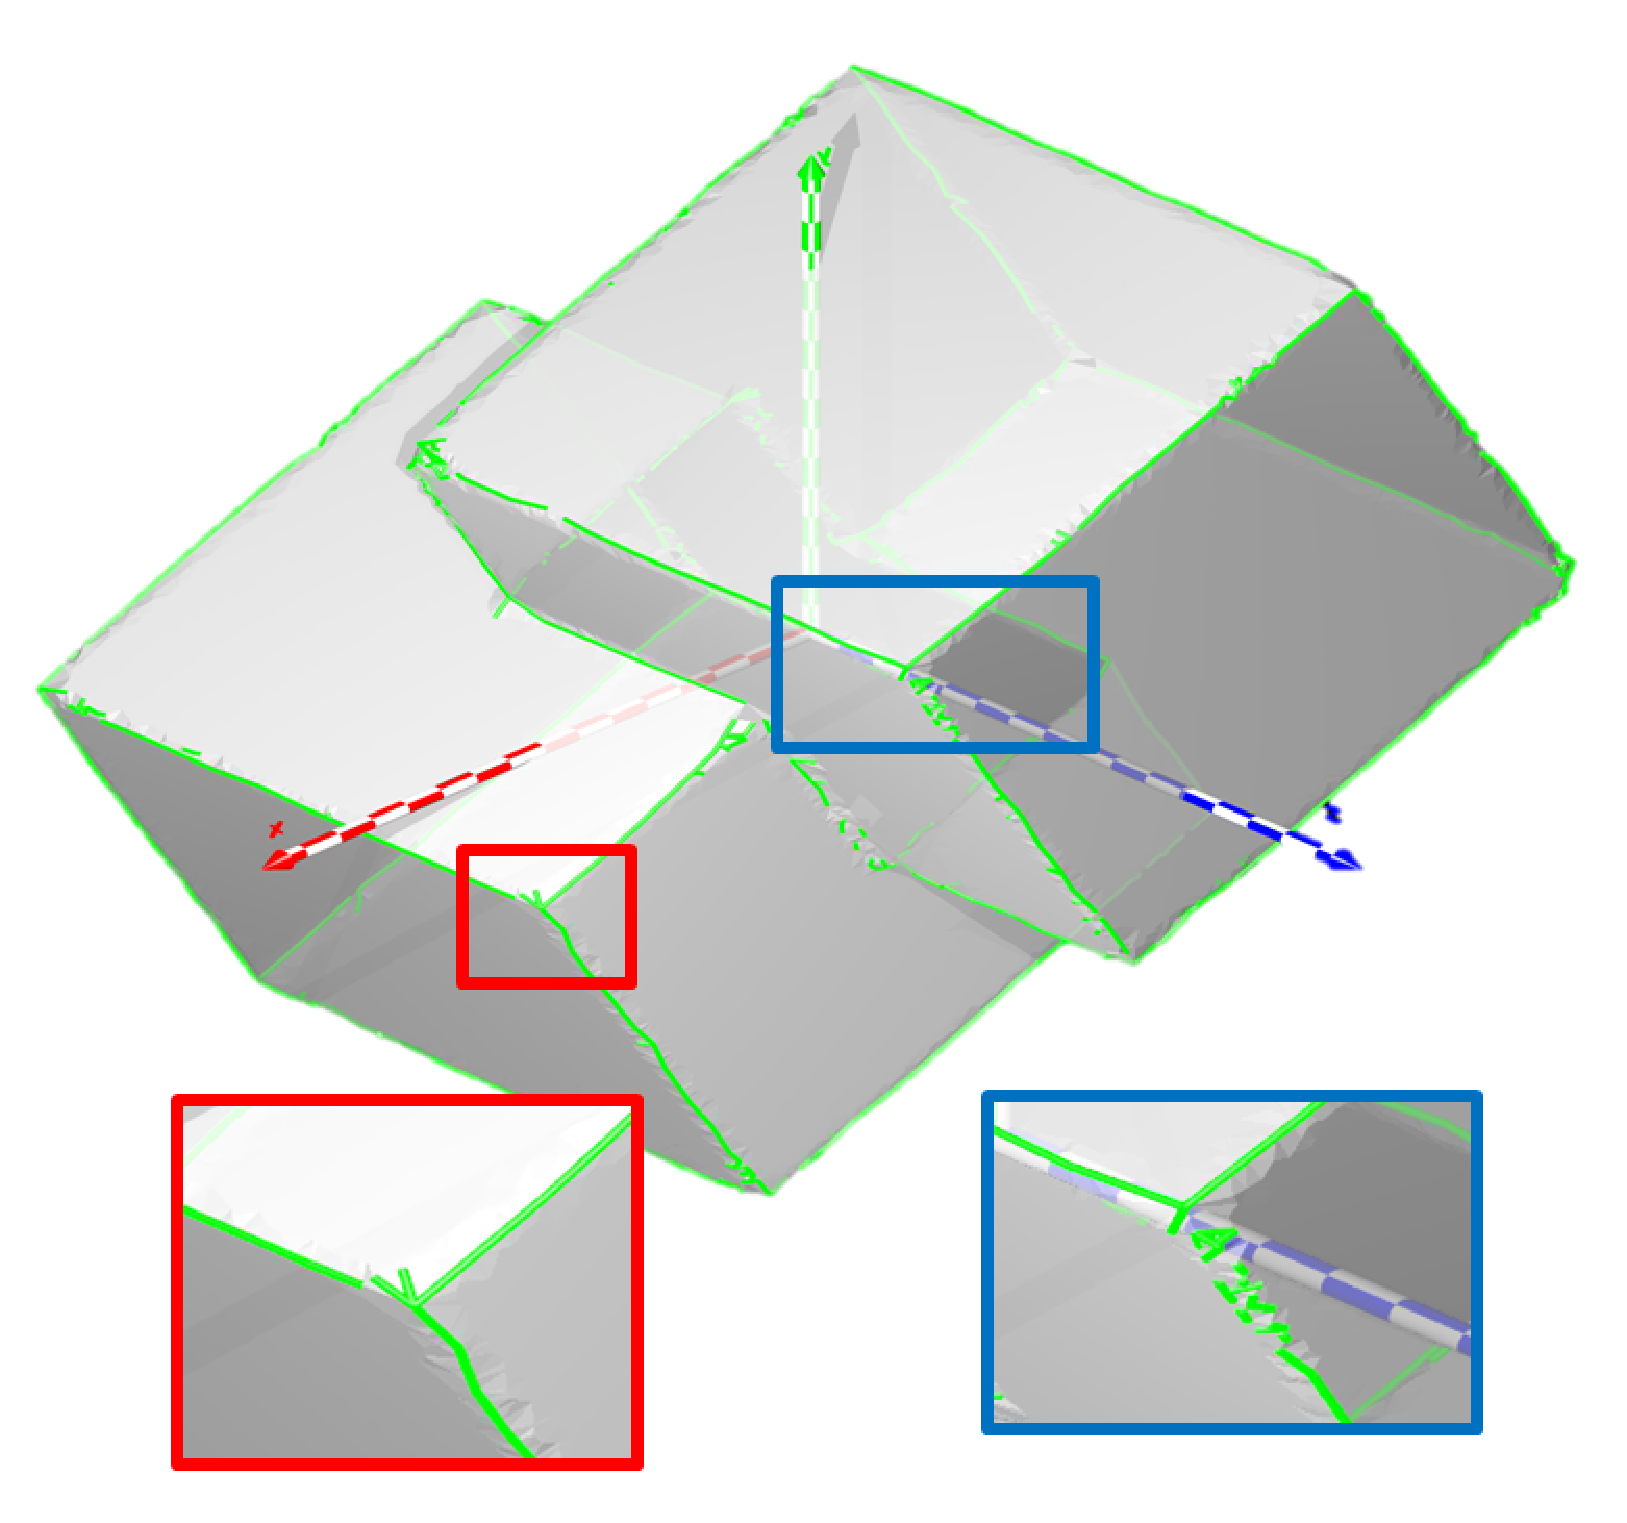
\includegraphics[width=0.5\linewidth]{images/compare_cocone_perfect_mc_b.eps}\label{fig:cocone_img:b}}
	%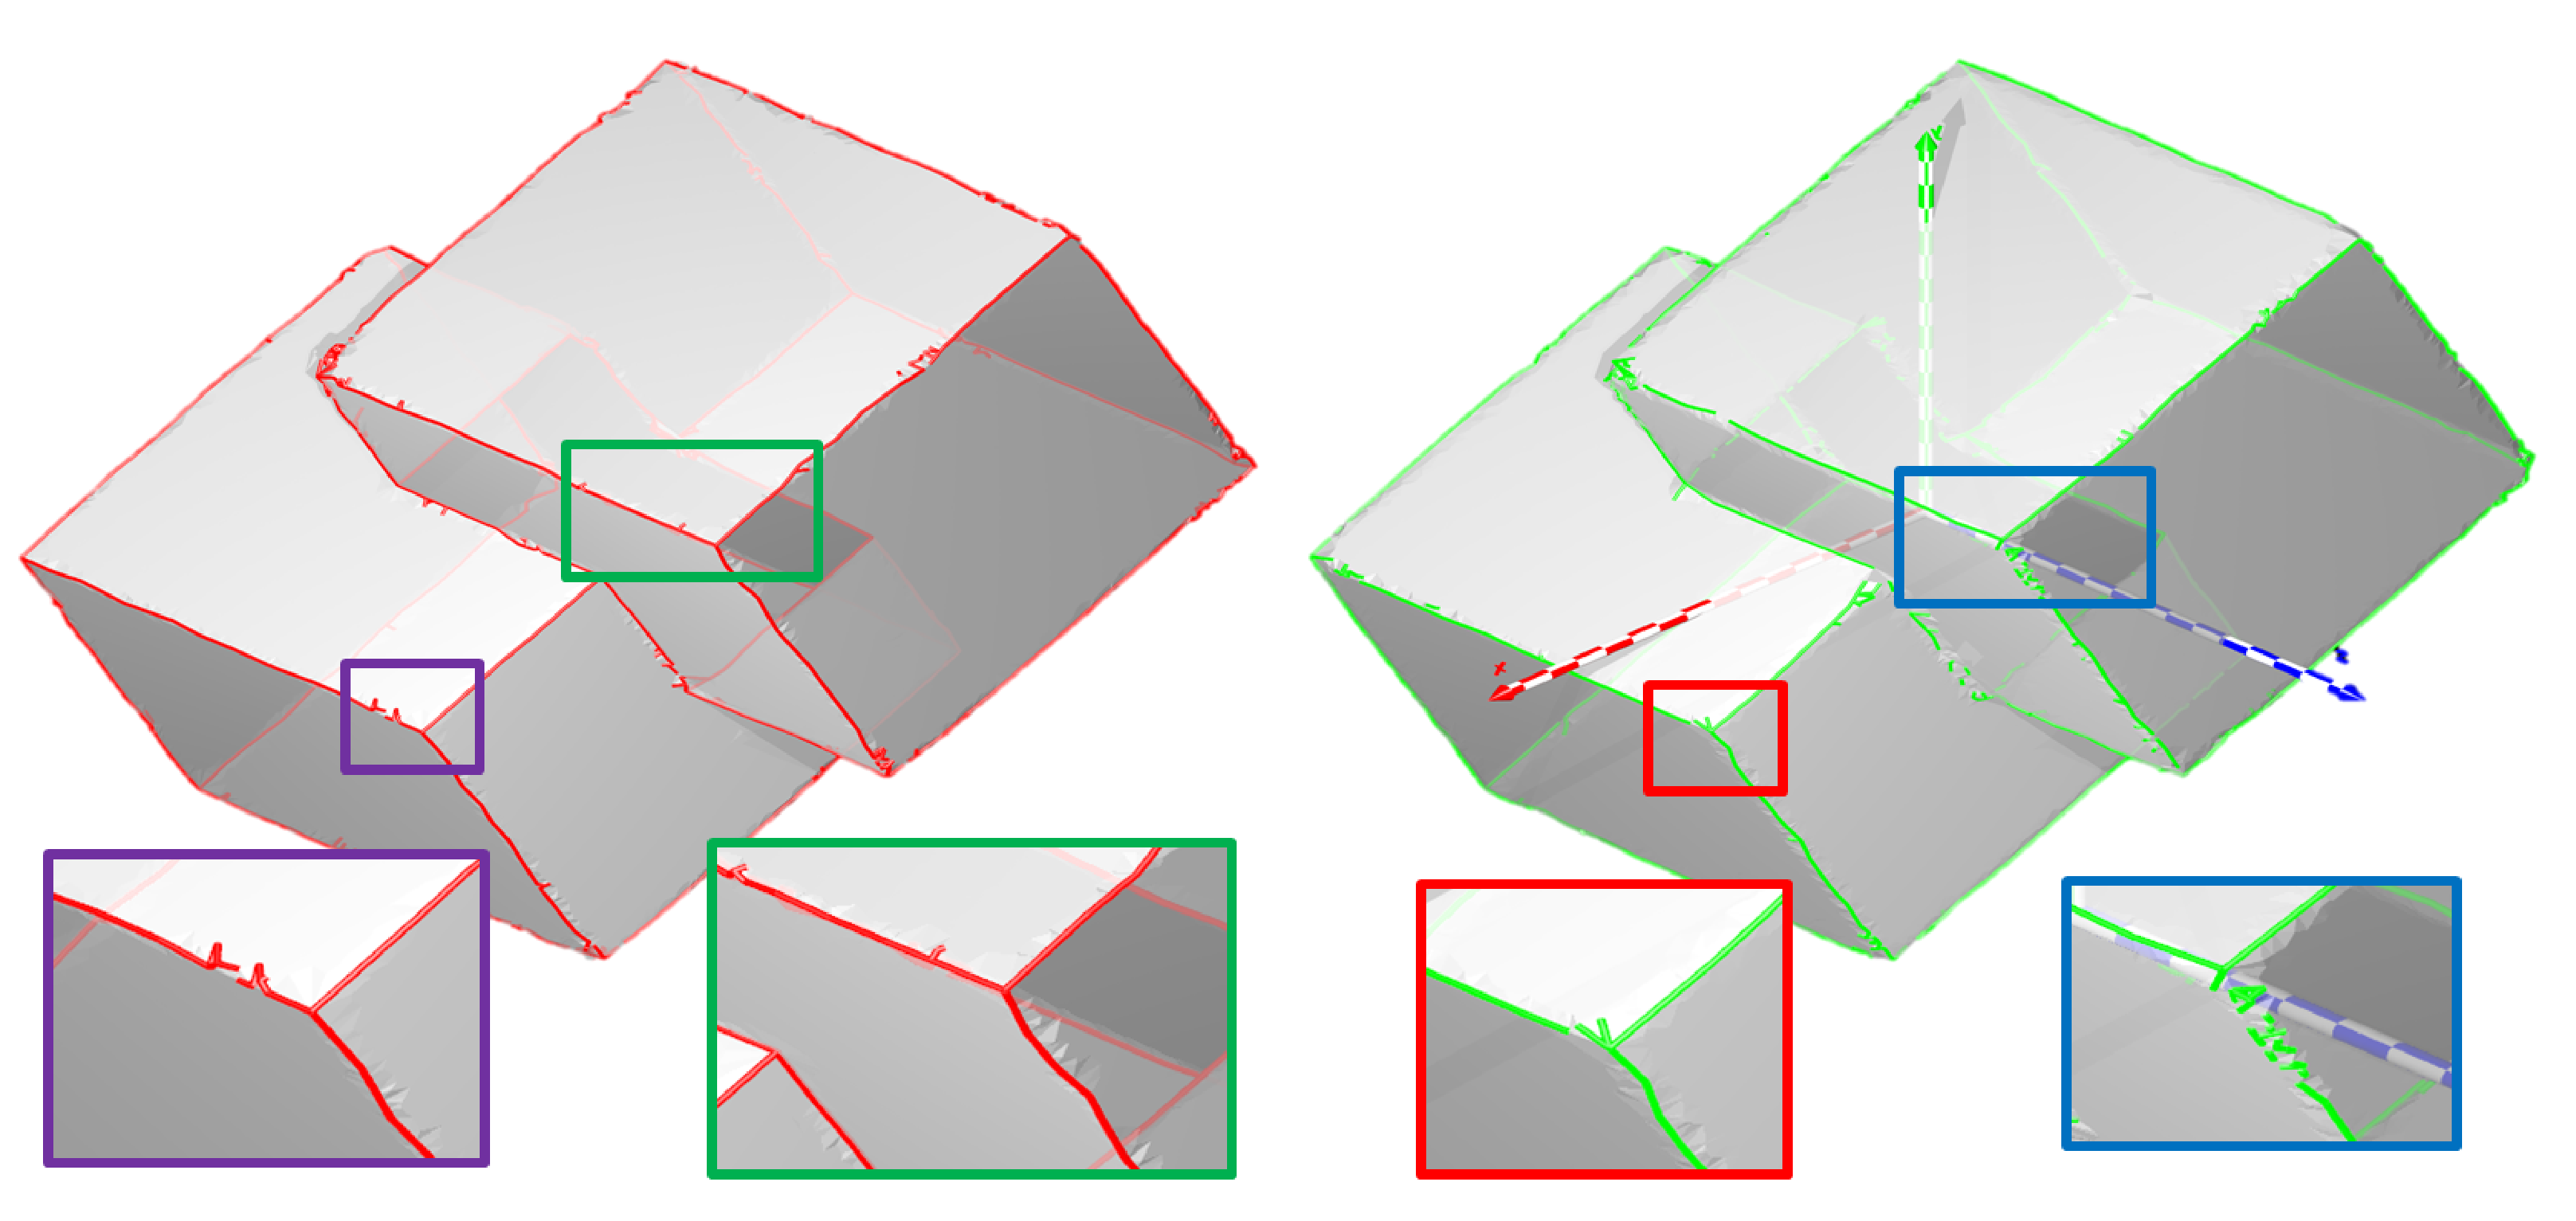
\includegraphics[width=\linewidth]{images/compare_cocone_perfect_mc.eps}
	\caption{Result of WeightCocone reconstruction on a TwoCube dataset. \protect\subref{fig:cocone_img:a} Input cloud is the super-sampled synthetic mesh. \protect\subref{fig:cocone_img:b} Input cloud is the super-sampled Marching Cube mesh. The magnified regions show some of the errors. The reconstruction from point cloud generated from the Marching Cube input is worse than the  point cloud from synthetic mesh input. }
	\label{fig:cocone_compare_from_perfect_1}
	\vskip-0.2cm
\end{figure} 

Figure~\ref{fig:cocone_compare_from_perfect_1} shows the reconstructed mesh for one of our twoCube dataset. The associated ``sharp" edges are also shown. Figure~\ref{fig:cocone_compare_from_perfect_1}(a) shows the reconstruction from the point cloud generated from the synthetic mesh. The overlay-ed ``sharp" edges (in red) show that the reconstruction has many errors. The magnified regions show some of the errors along the sharp edges and corners. Figure~\ref{fig:cocone_compare_from_perfect_1}(b) shows the reconstruction from the point cloud generated from running Marching Cubes. The magnified regions show the same regions as Figure~\ref{fig:cocone_compare_from_perfect_1}(a). The reconstruction is worse than WeightCocone using input from synthetic mesh. 

Figure~\ref{fig:cocone:compare} shows the summary results of running weightCocone and SHREC on 15 different datasets. 
The input to weightCocone  for these tests are generated from synthetic mesh. The results from Marching Cubes input are worse and not shown.
\paragraph{}
On the same 15 datasets, we run SHREC with both synthetic gradients and using RELIGRAD.
Figure~\protect\subref*{fig:cocone:a} shows countDegree error comparison between WeightCocone, SHREC with synthetic gradient and SHREC with gradient computed using RELIGRAD.  SHREC with RELIGRAD generates very few errors, while with synthetic gradient no errors are generated. 
In contrast WeightCocone generates a large number of errors on all the testcases. Figure~\protect\subref*{fig:cocone:b} shows the maximum surface angle difference from the synthetic mesh for SHREC with RELIGRAD and WeighCocone; the angle difference from the WeightCocone is very large in all the tests. Figure~\protect\subref*{fig:cocone:c} shows the angle distribution for WeightCocone construction on the 15 testcases. 
On all the test cases there are large number of simplices with angle difference more than 40$^\circ$ and 50$^\circ$.

This quantitatively shows what we saw in Figure~\protect\subref*{fig:cocone_img:a},~\protect\subref*{fig:cocone_img:b} and Figure~\ref{fig:shrecPerfect1},~\ref{fig:flange1} i.e sharp edges generated by WeightCocone is in general worse than those generated by SHREC with synthetic as well as RELIGRAD gradients. 

Dey et al.~\cite{Dey2012,Dey2013} report better results on their datasets, Which might possibly be because of parameter tuning. They themselves acknowledged as such in their work.
\begin{figure*}[htb]
	\centering
		\subfloat[]{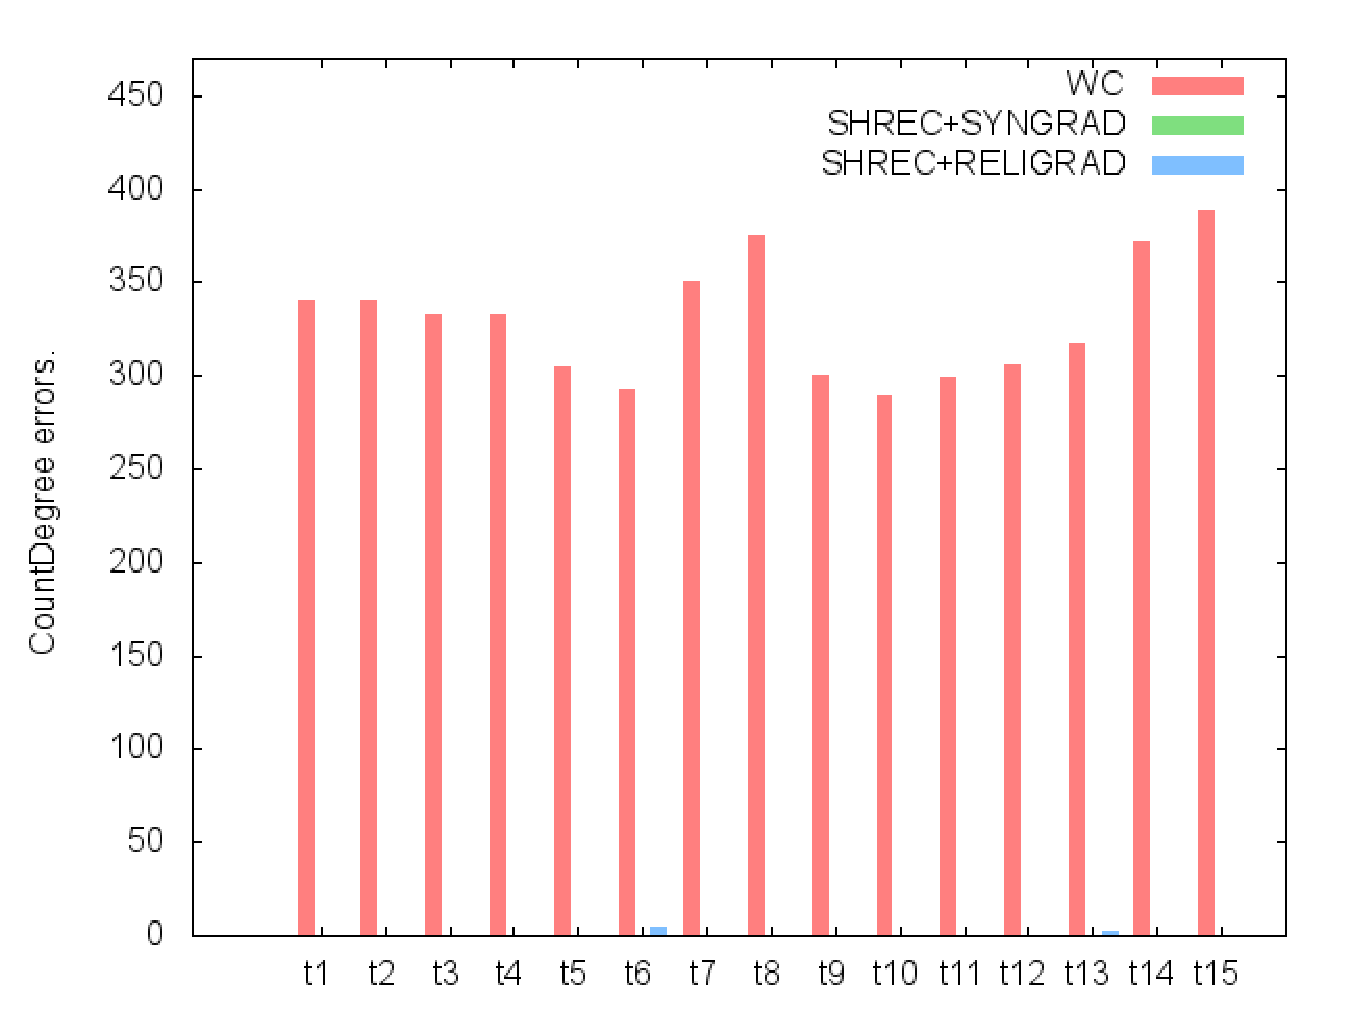
\includegraphics[width=0.3\linewidth]{images/cocone_cd_twoCube.eps}\label{fig:cocone:a}}
		\subfloat[]{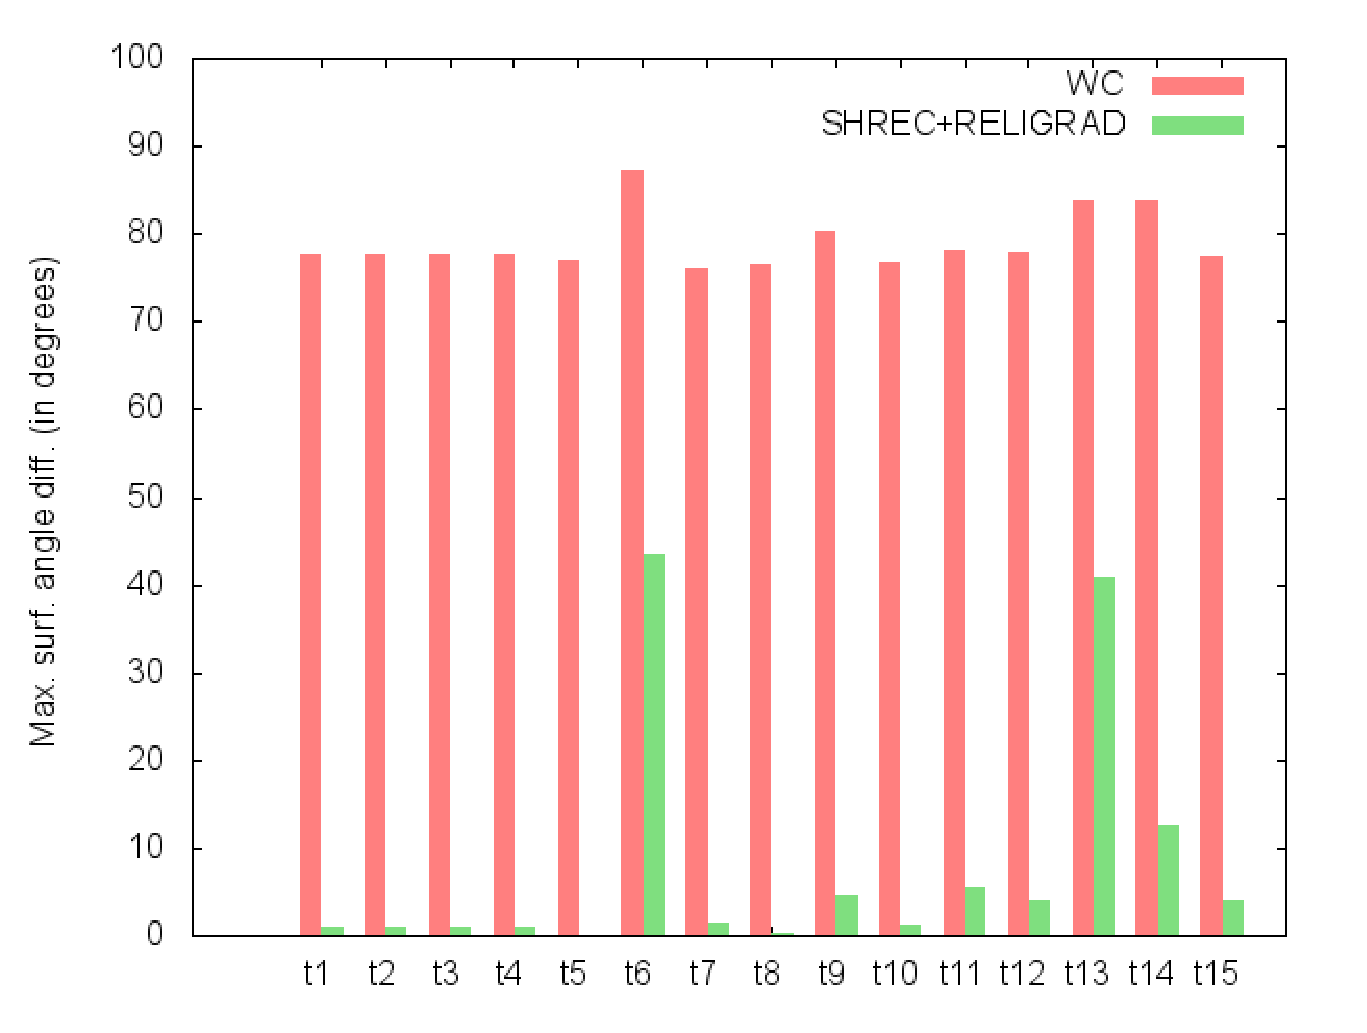
\includegraphics[width=0.3\linewidth]{images/cocone_max_angle_twoCube.eps}\label{fig:cocone:b}}	
		\subfloat[]{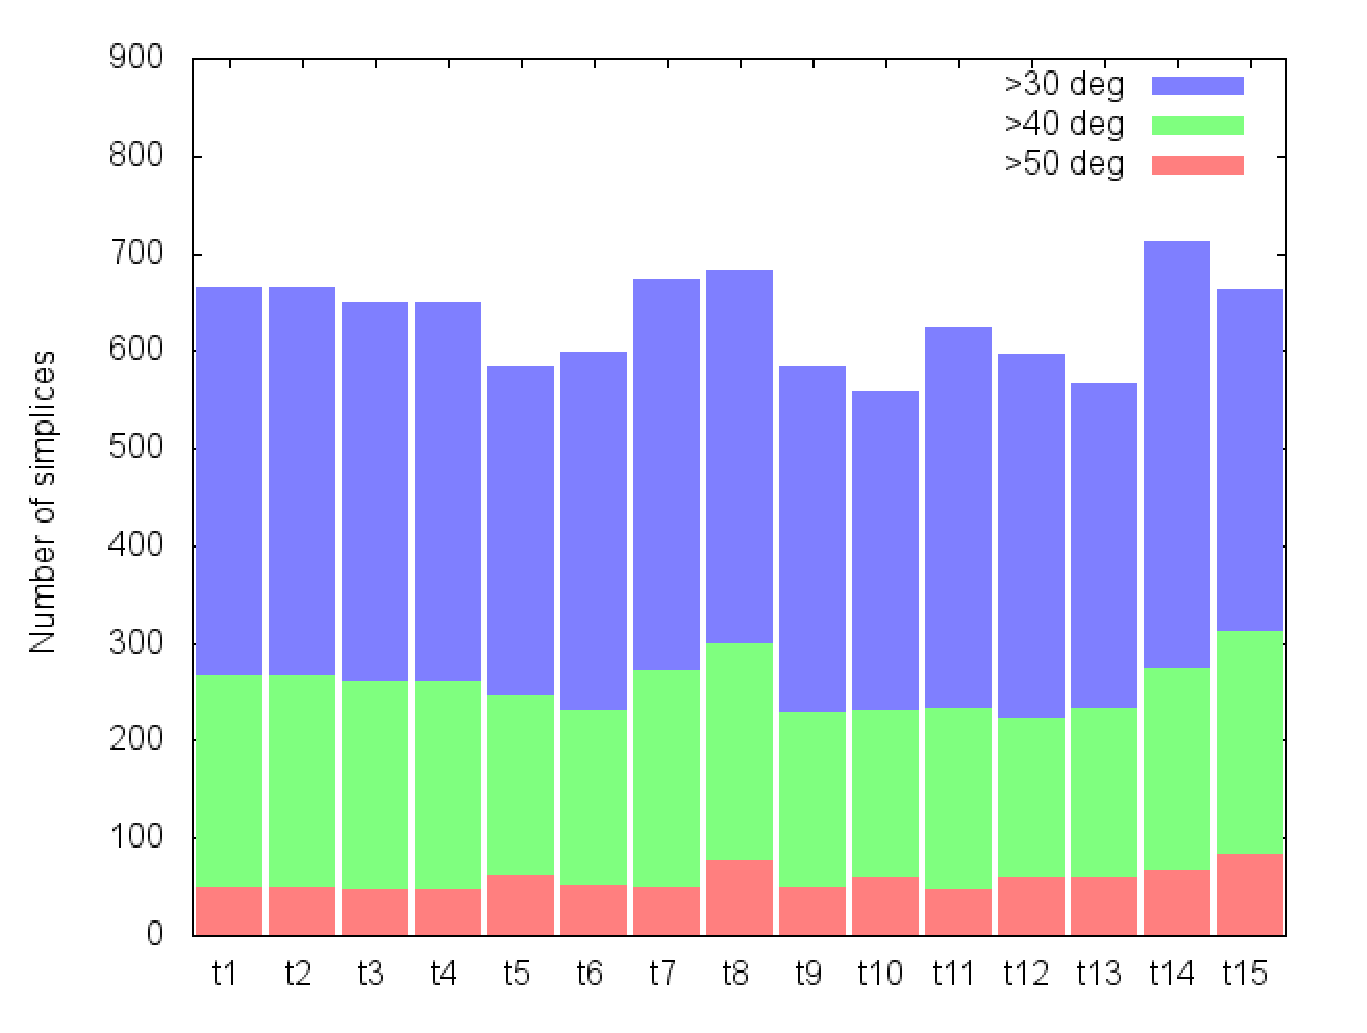
\includegraphics[width=0.3\linewidth]{images/cocone_angle_distri_twoCube.eps}\label{fig:cocone:c}}		
		%\subfloat[]{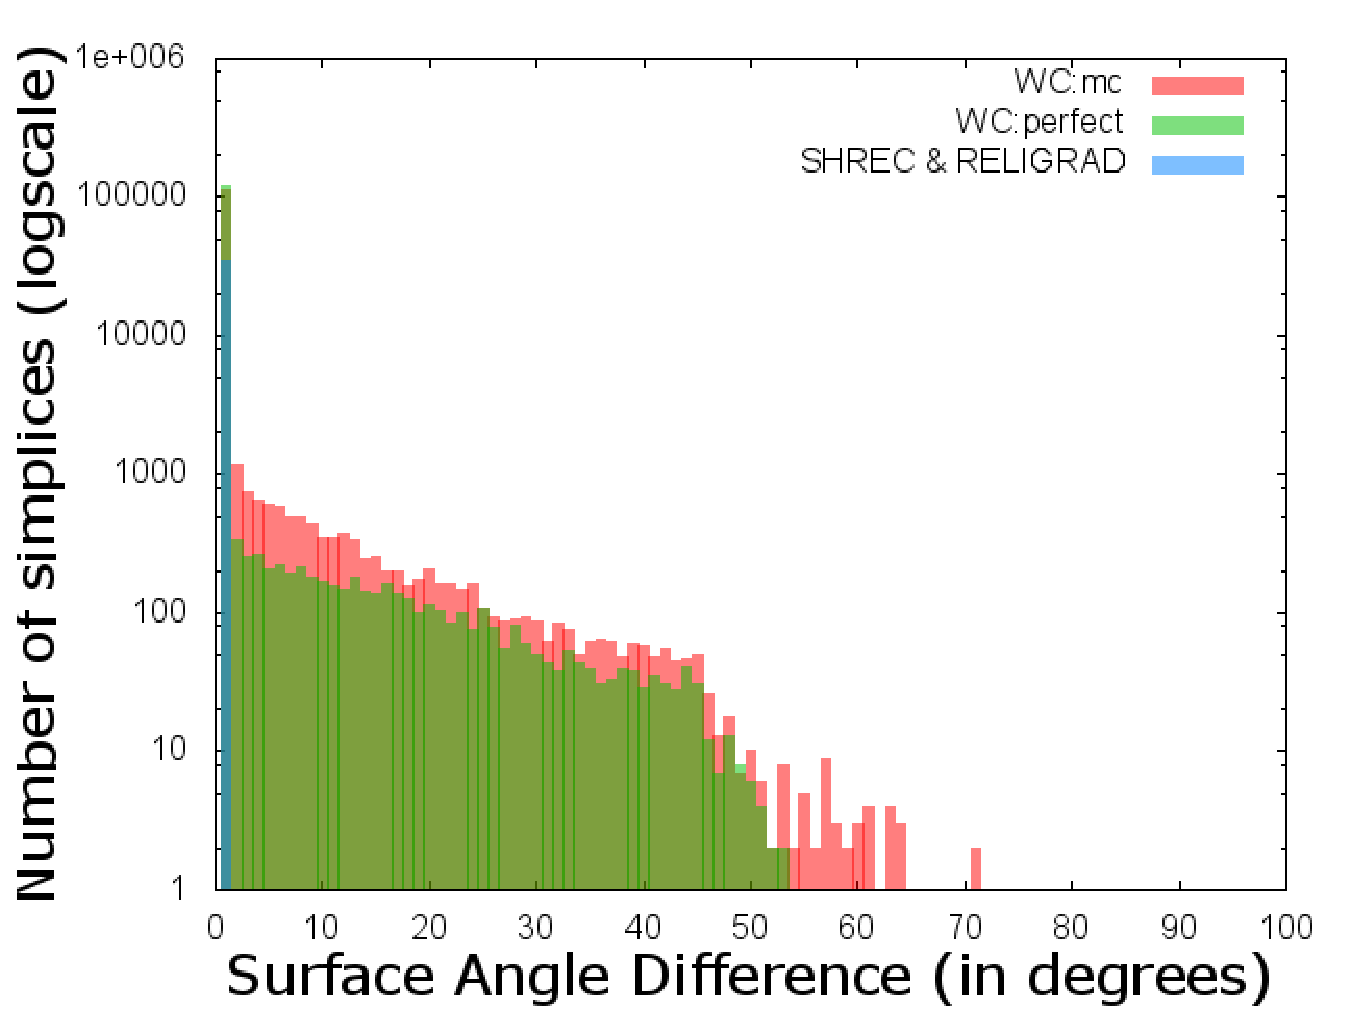
\includegraphics[width=0.6\linewidth]{images/twoCubeQuant.eps}\label{table:cocone_compare_with_mc_table_1}}
		\caption{Cocone comparison Dey et al.~\cite{Dey2012,Dey2013}.(a) CountDegree errors on 15 datasets using SHREC with synthetic gradients, RELIGRAD and WeightCocone. (b)Max. surface angle difference for the 15 testcases using WeightCocone and SHREC (c) Number of simplices with angle difference of 30$^\circ$, 40$^\circ$ and 50$^\circ$ from the original mesh on a subset of 15 datasets using WeightCocone with  input points sampled from the synthetic mesh.}
		\label{fig:cocone:compare}
\end{figure*}
\paragraph{Polymender comparison;}
We next compared SHREC to Polymender. Polymender is an implementation of mesh repairing algorithm from Ju~\cite{j-rrpm-04} availiable at \url{www.cse.wustl.edu/~taoju/code/polymender.htm} \href{http://www.cse.wustl.edu/~taoju/code/polymender.htm}{}. 
We ran the 34 twocube datasets and the 34 flange dataset using Polymender. 

Figure~\ref{fig:polymenderA} shows the summary results both using CountDegree and surface angle differences.
Figure~\ref{fig:polymenderB} shows qualitatively comparison between Polymender and SHREC. 
Figure~\protect\subref*{fig:polymender:a},~\protect\subref*{fig:polymender:b} and ~\protect\subref*{fig:polymender:f} shows the countDegree errors, the maximum surface angle difference from the synthetic mesh and the angle distribution for 34 twoCube datasets respectively. Similarly, 
Figure~\protect\subref*{fig:polymender:c},~\protect\subref*{fig:polymender:d} and ~\protect\subref*{fig:polymender:e} shows the results for the 34 flange datasets. Polymender produces numerous degree errors both in flange and twoCube datasets. The maximum degree error for twoCube datasets, is ~170. At least 3 flange dataset produce over 350 errors. Both Flange and twoCube produce large maximum angle difference errors from the synthetic mesh. The angle distributions show the angle errors are not isolated instead large number of simplices in both the flange and the twoCube datasets have large (over 50$^\circ$) angle difference from the synthetic mesh.    

Figure~\protect\subref*{fig:polymenderB:a} shows part of a flange dataset reconstructed using SHREC and RELIGRAD. Figure~\protect\subref*{fig:polymenderB:b} shows the same region reconstructed using Polymender; note the ``flipped" triangle and distorted ``sharp" line. Figure~\protect\subref*{fig:polymenderB:c} shows the surface angle  difference distribution for the meshes shown in Figure~\protect\subref*{fig:polymenderB:a} and Figure~\protect\subref*{fig:polymenderB:b}; as expected SHREC produces far few large angle difference than Polymender.

Figure~\protect\subref*{fig:polymender:cone:a} shows a cone dataset reconstructed using SHREC and RELIGRAD. Figure~\protect\subref*{fig:polymender:cone:b} shows the same dataset reconstructed using Polymender. The curved edges are not reconstructed accurately in Polymender. Figure~\protect\subref*{fig:polymender:cone:c} shows a close up comparison of the sharp edge reconstructed from SHREC(right) and Polymender(left). The sharp edge is not preserved when using Polymender.  We used the following parameters to run Polymender; ``octree depth" was set to 7 and ``scale" was set to 0.9 for all tests. 

\begin{figure*}[htb]
	\centering
		\subfloat[]{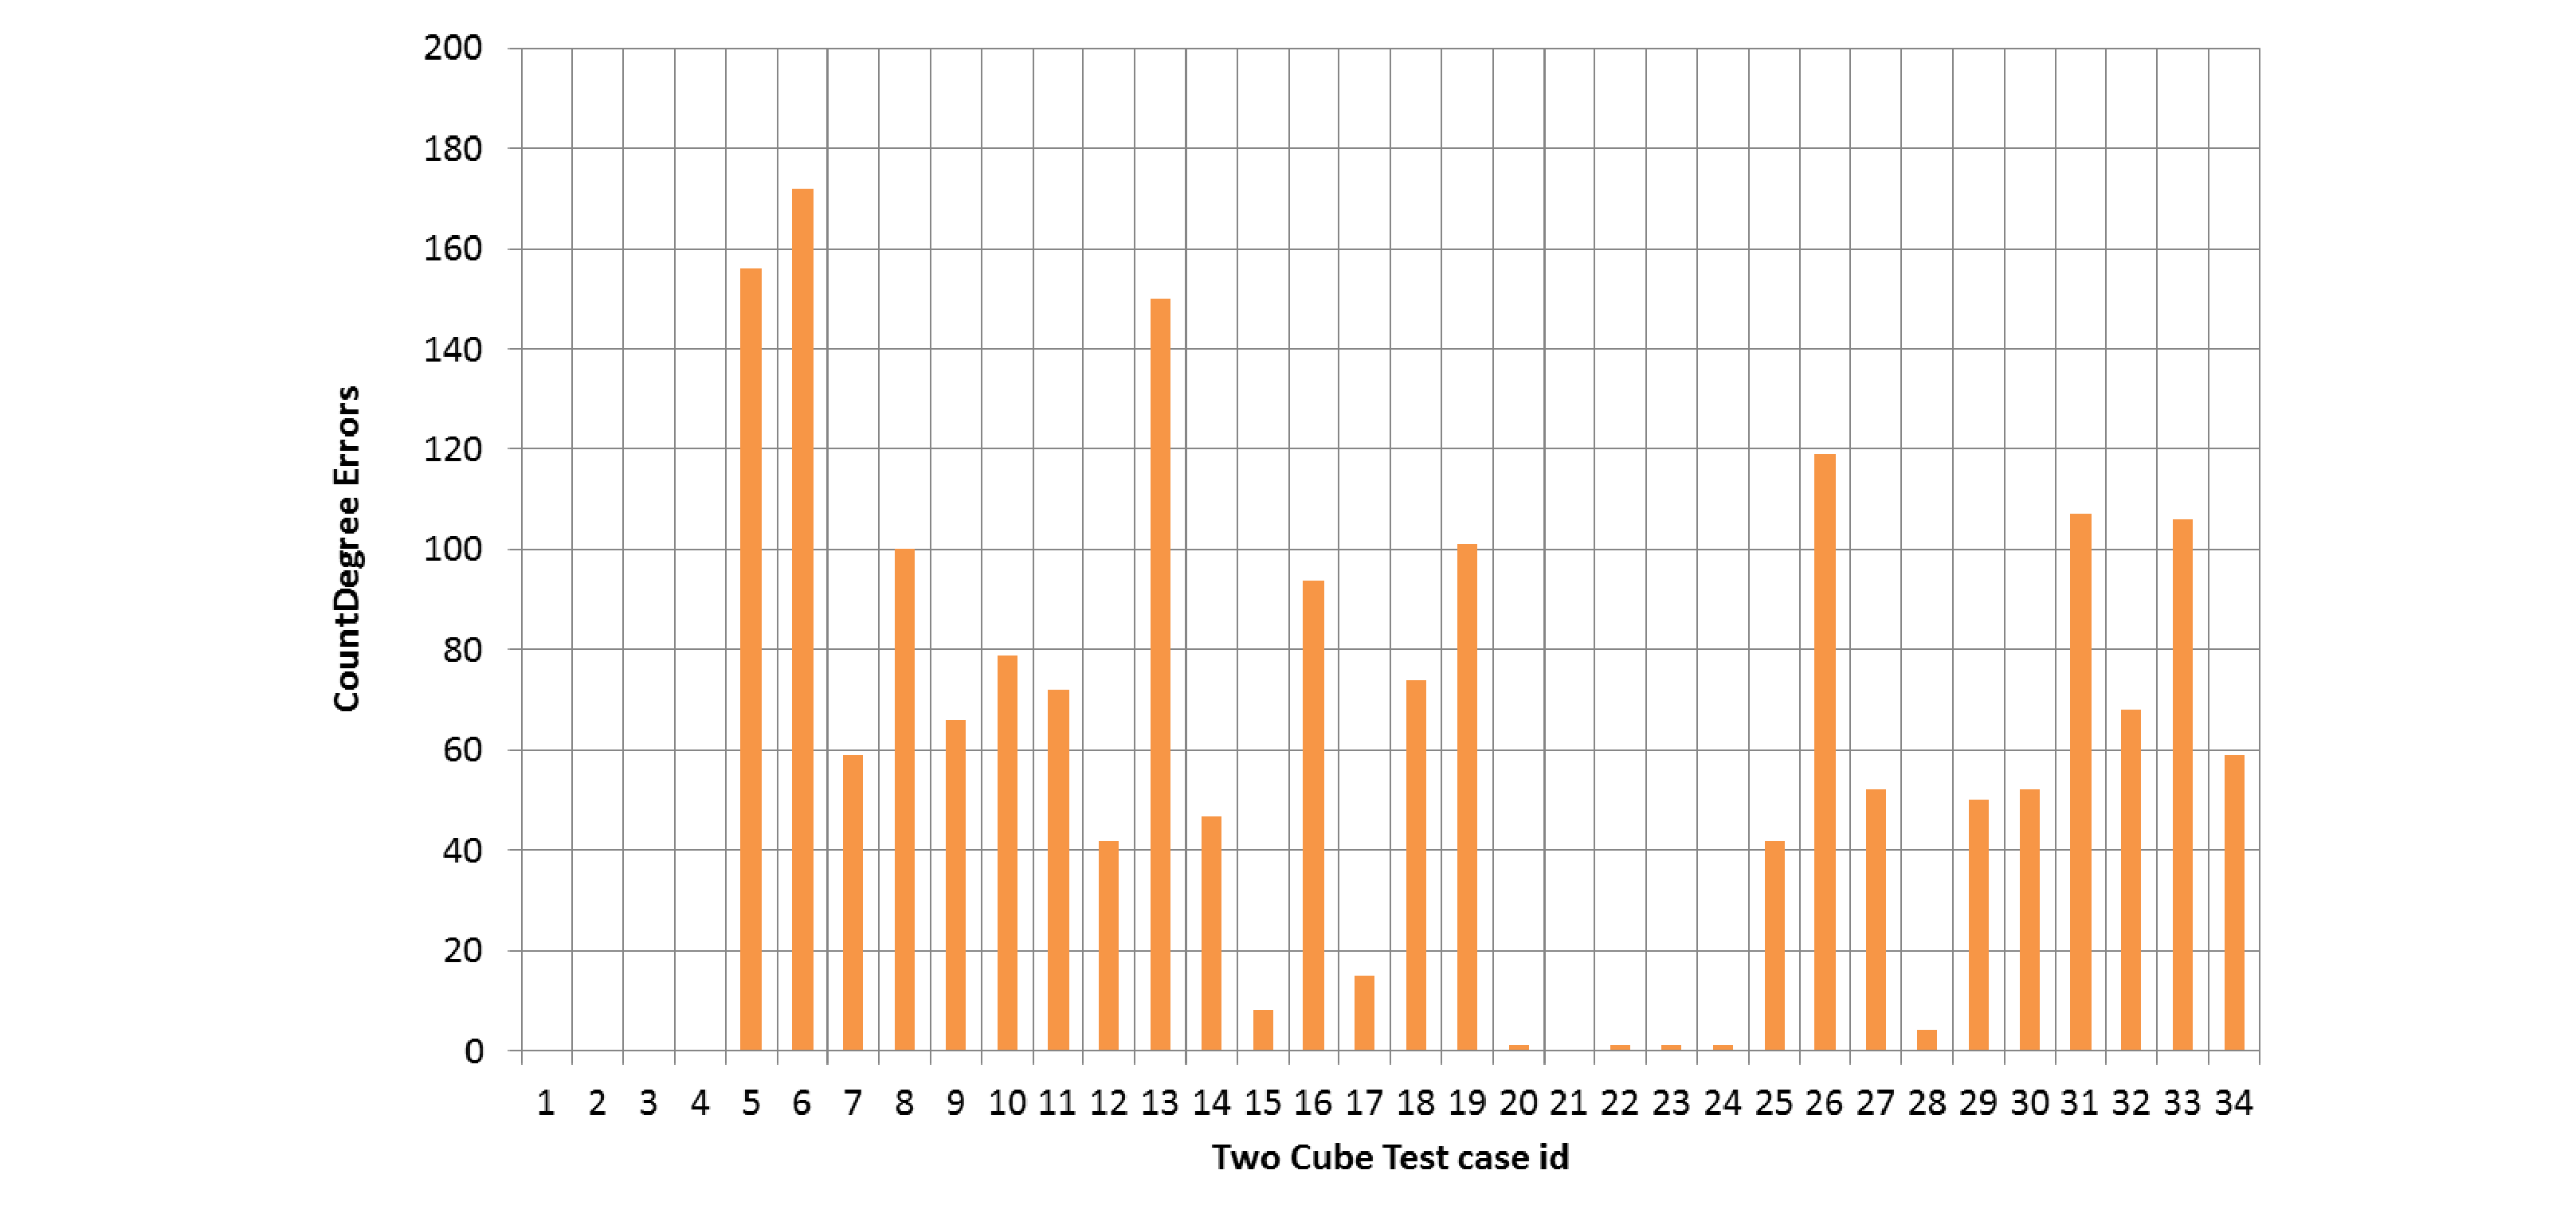
\includegraphics[trim={5cm 0 5cm 0},clip, width=0.45\linewidth]{images/twoCube_summary_2.eps}\label{fig:polymender:a}}\quad
				\subfloat[]{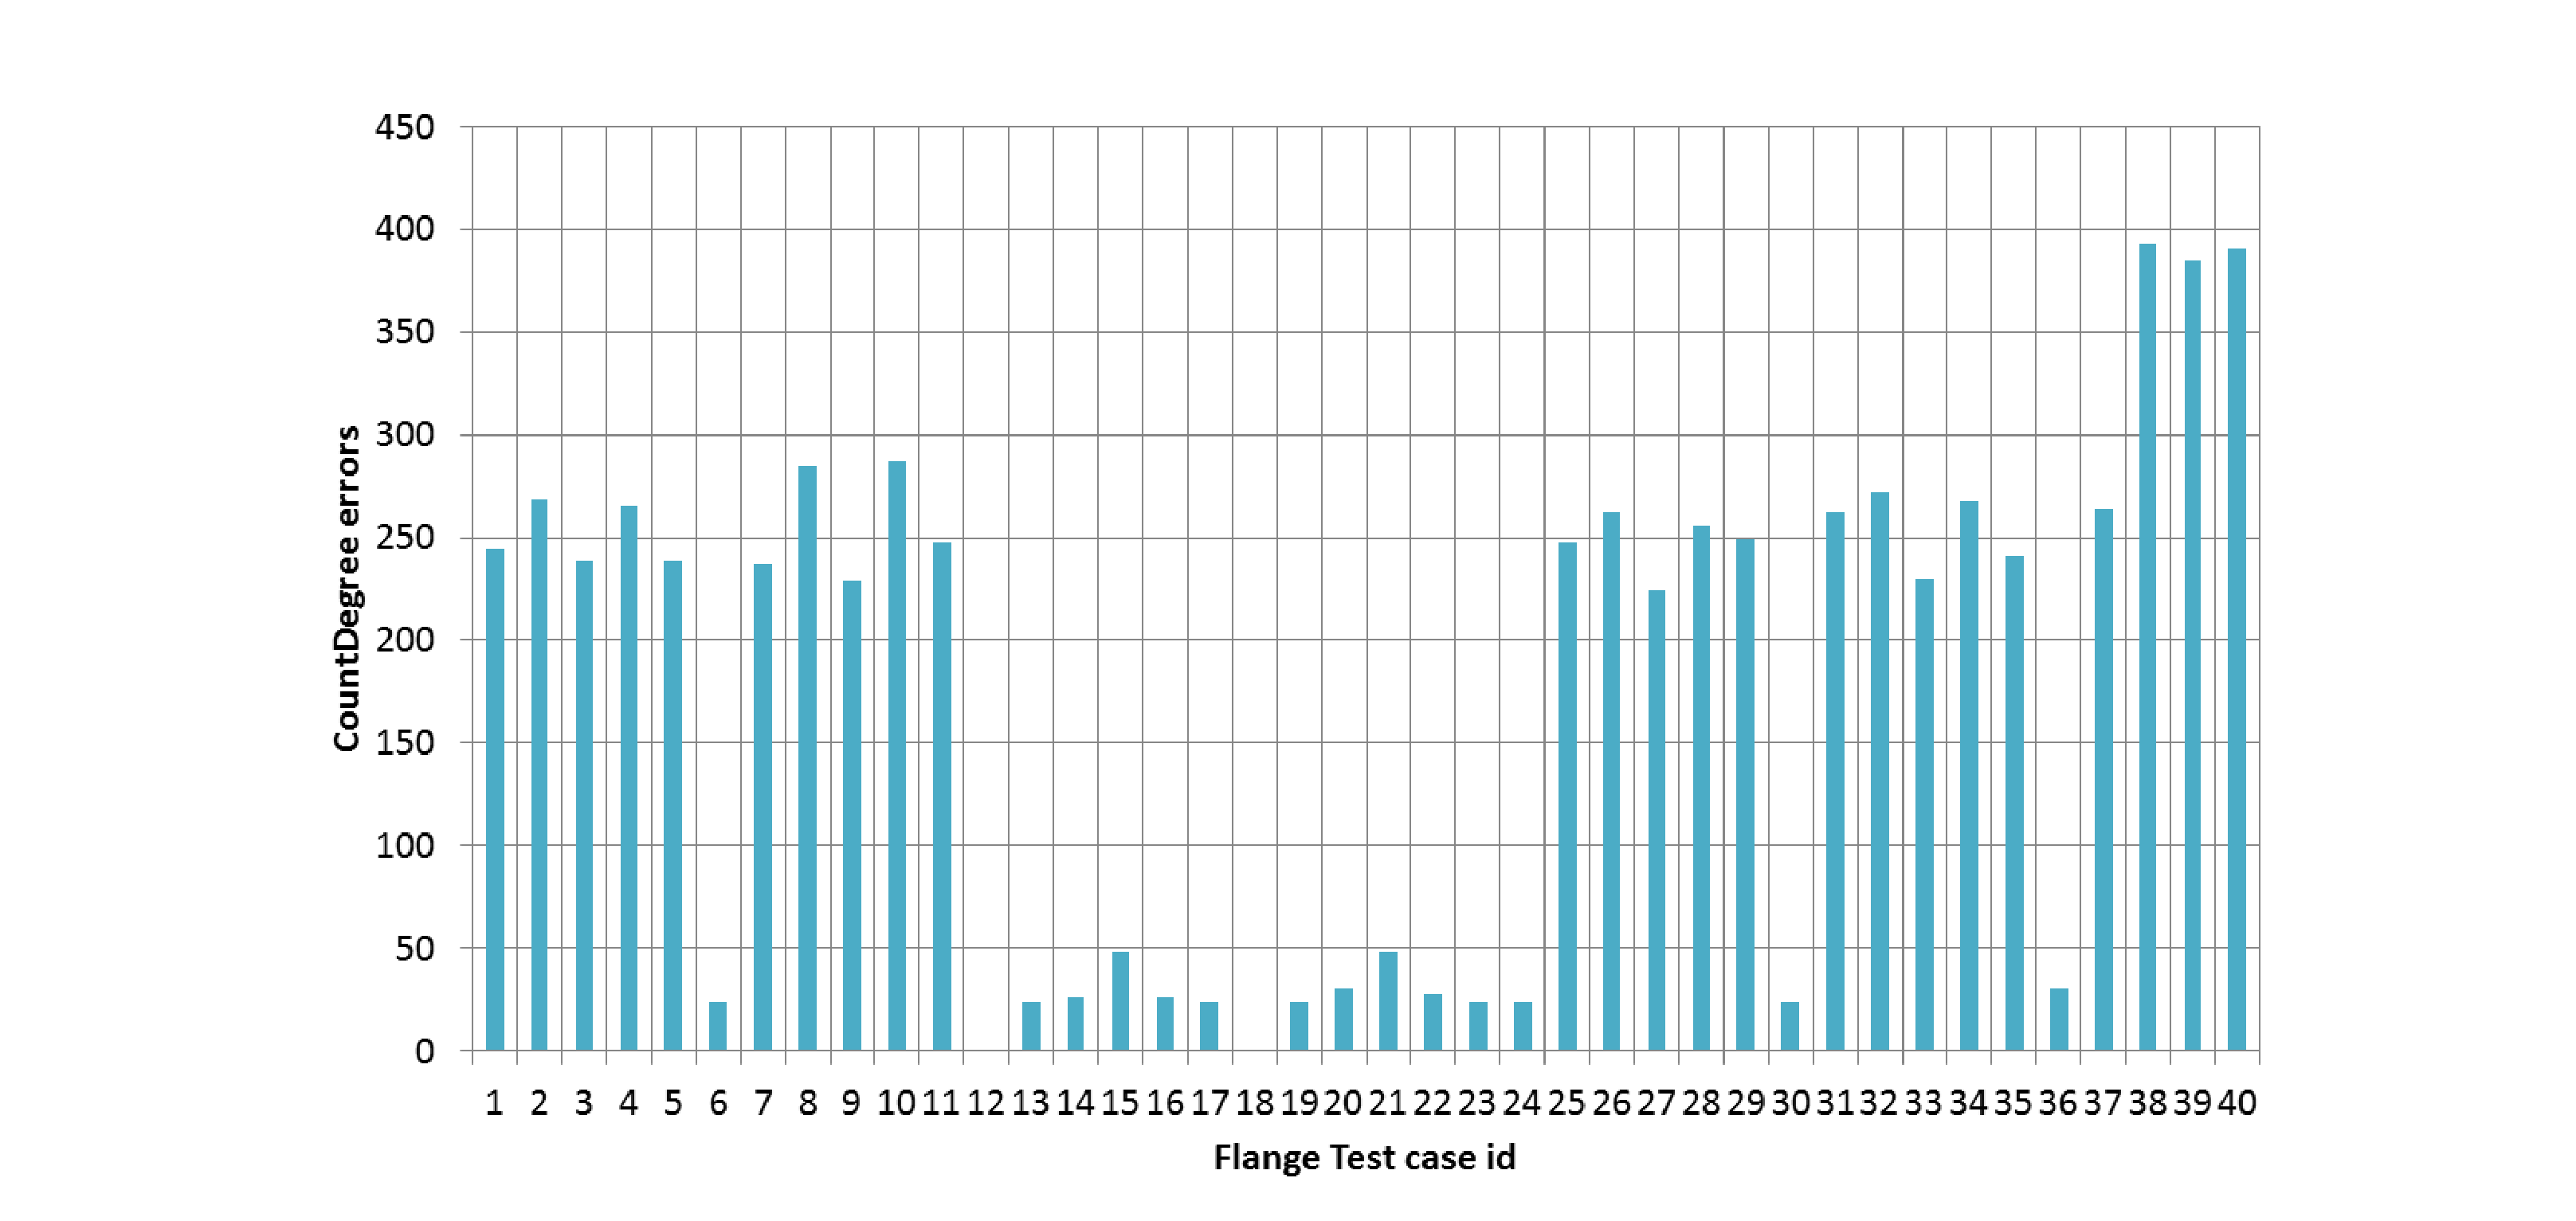
\includegraphics[trim={5cm 0 5cm 0},clip, width=0.45\linewidth]{images/countDegree_Flange.eps}\label{fig:polymender:c}}\\
		\subfloat[]{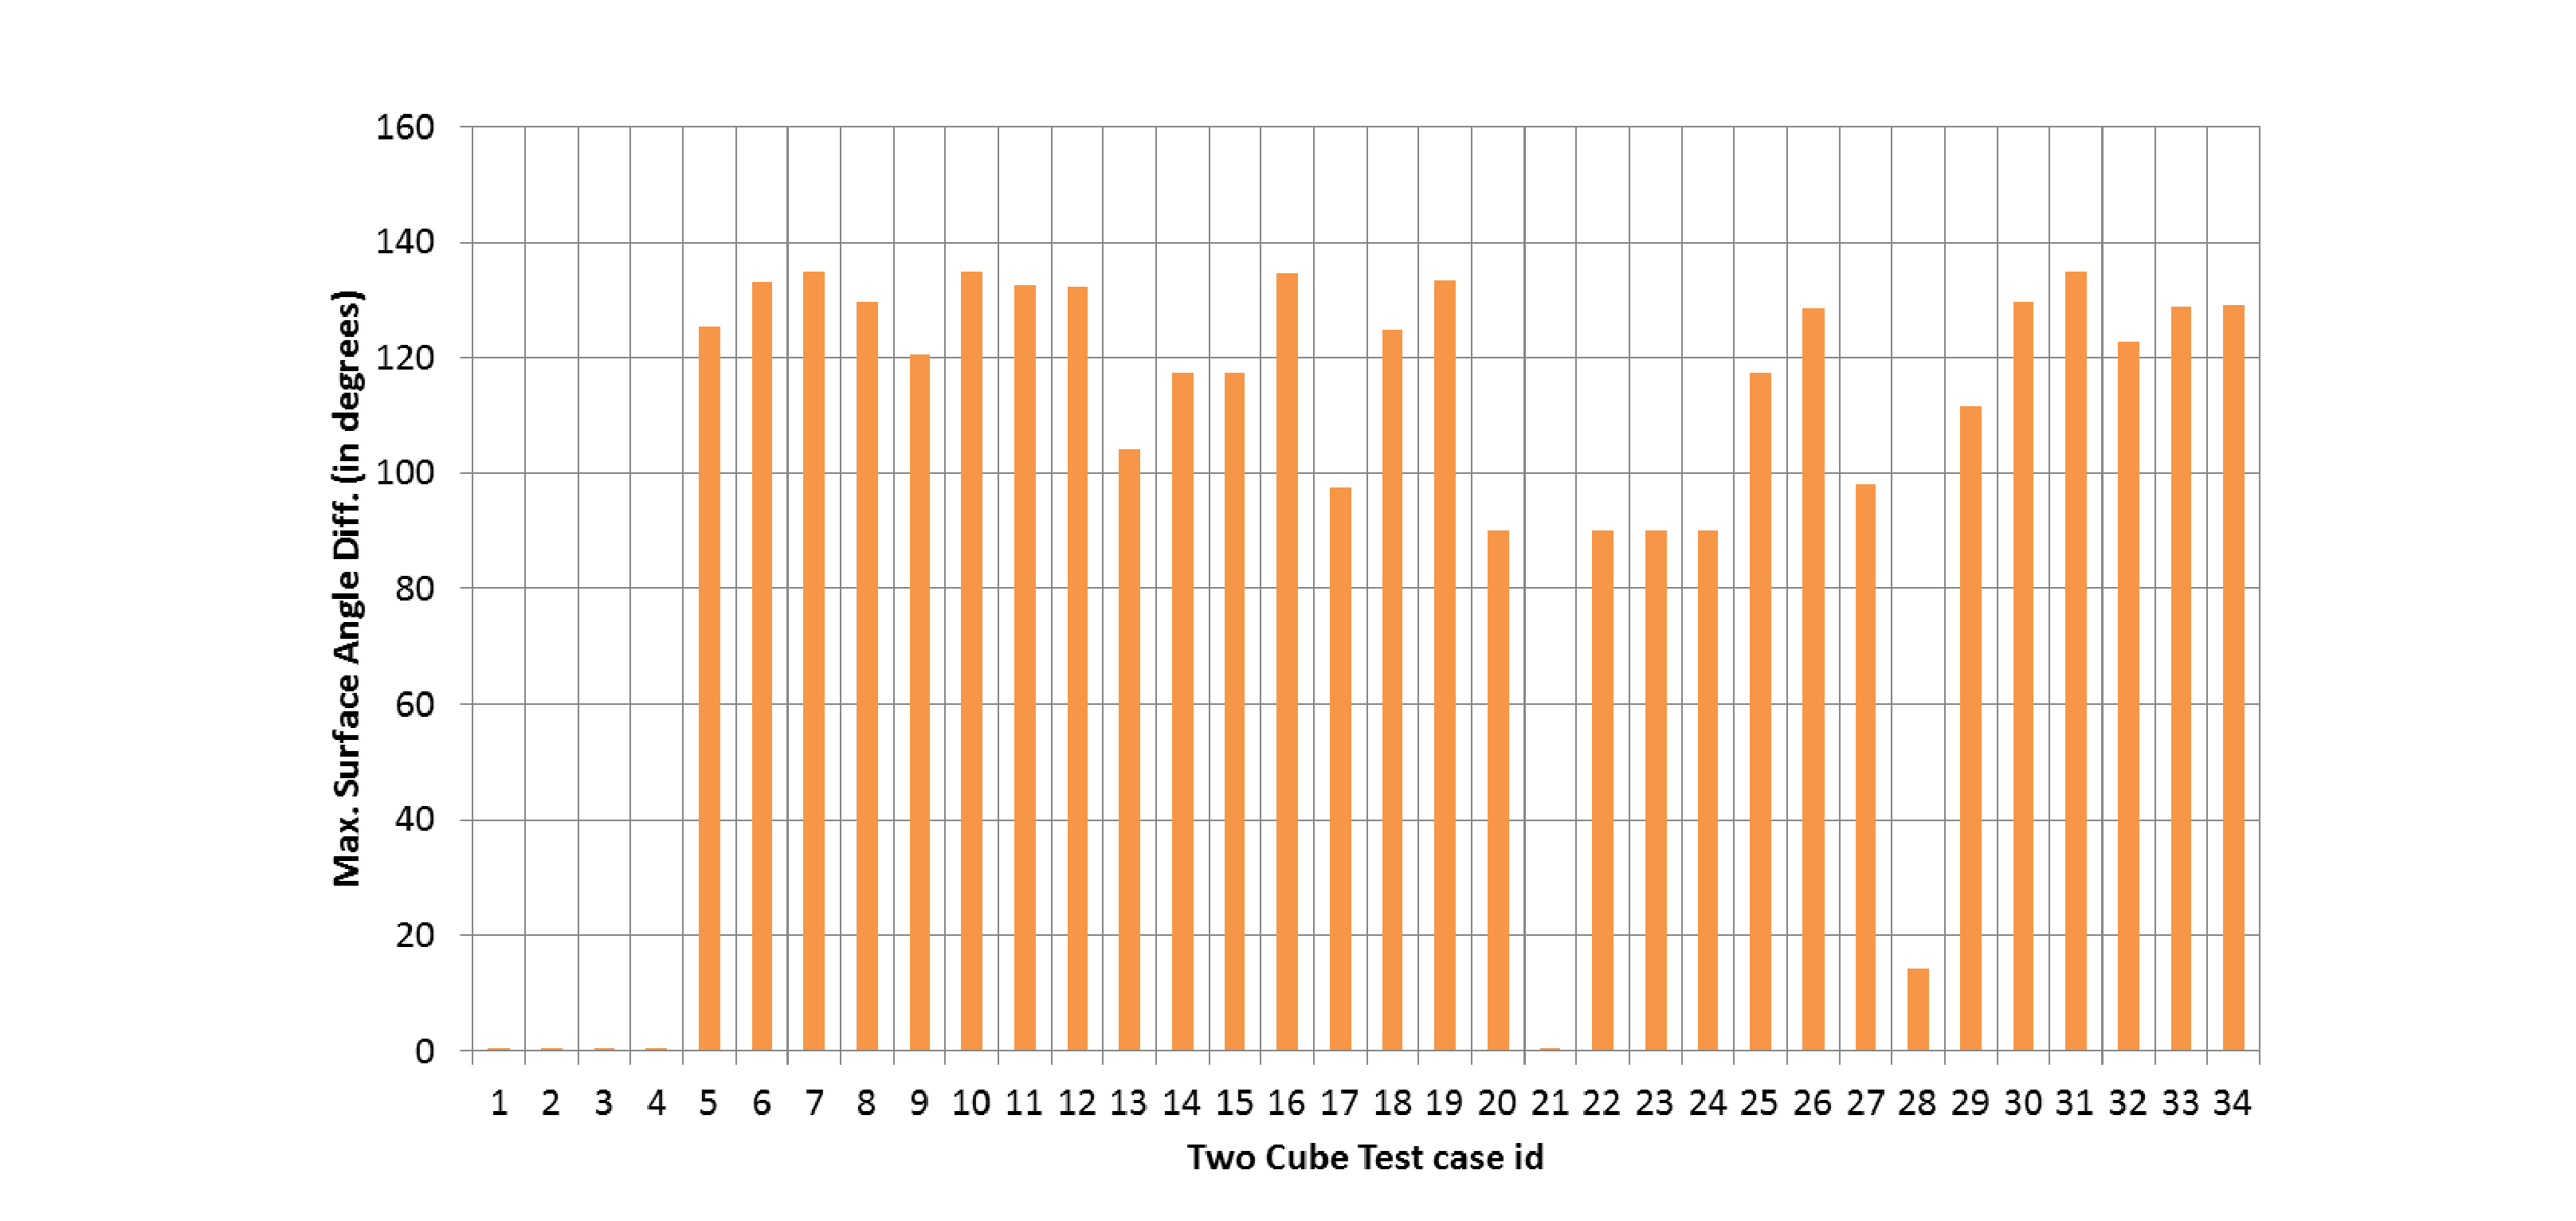
\includegraphics[trim={5cm 0 5cm 0},clip, width=0.45\linewidth]{images/twoCube_summary_1.eps}\label{fig:polymender:b}}\quad
		\subfloat[]{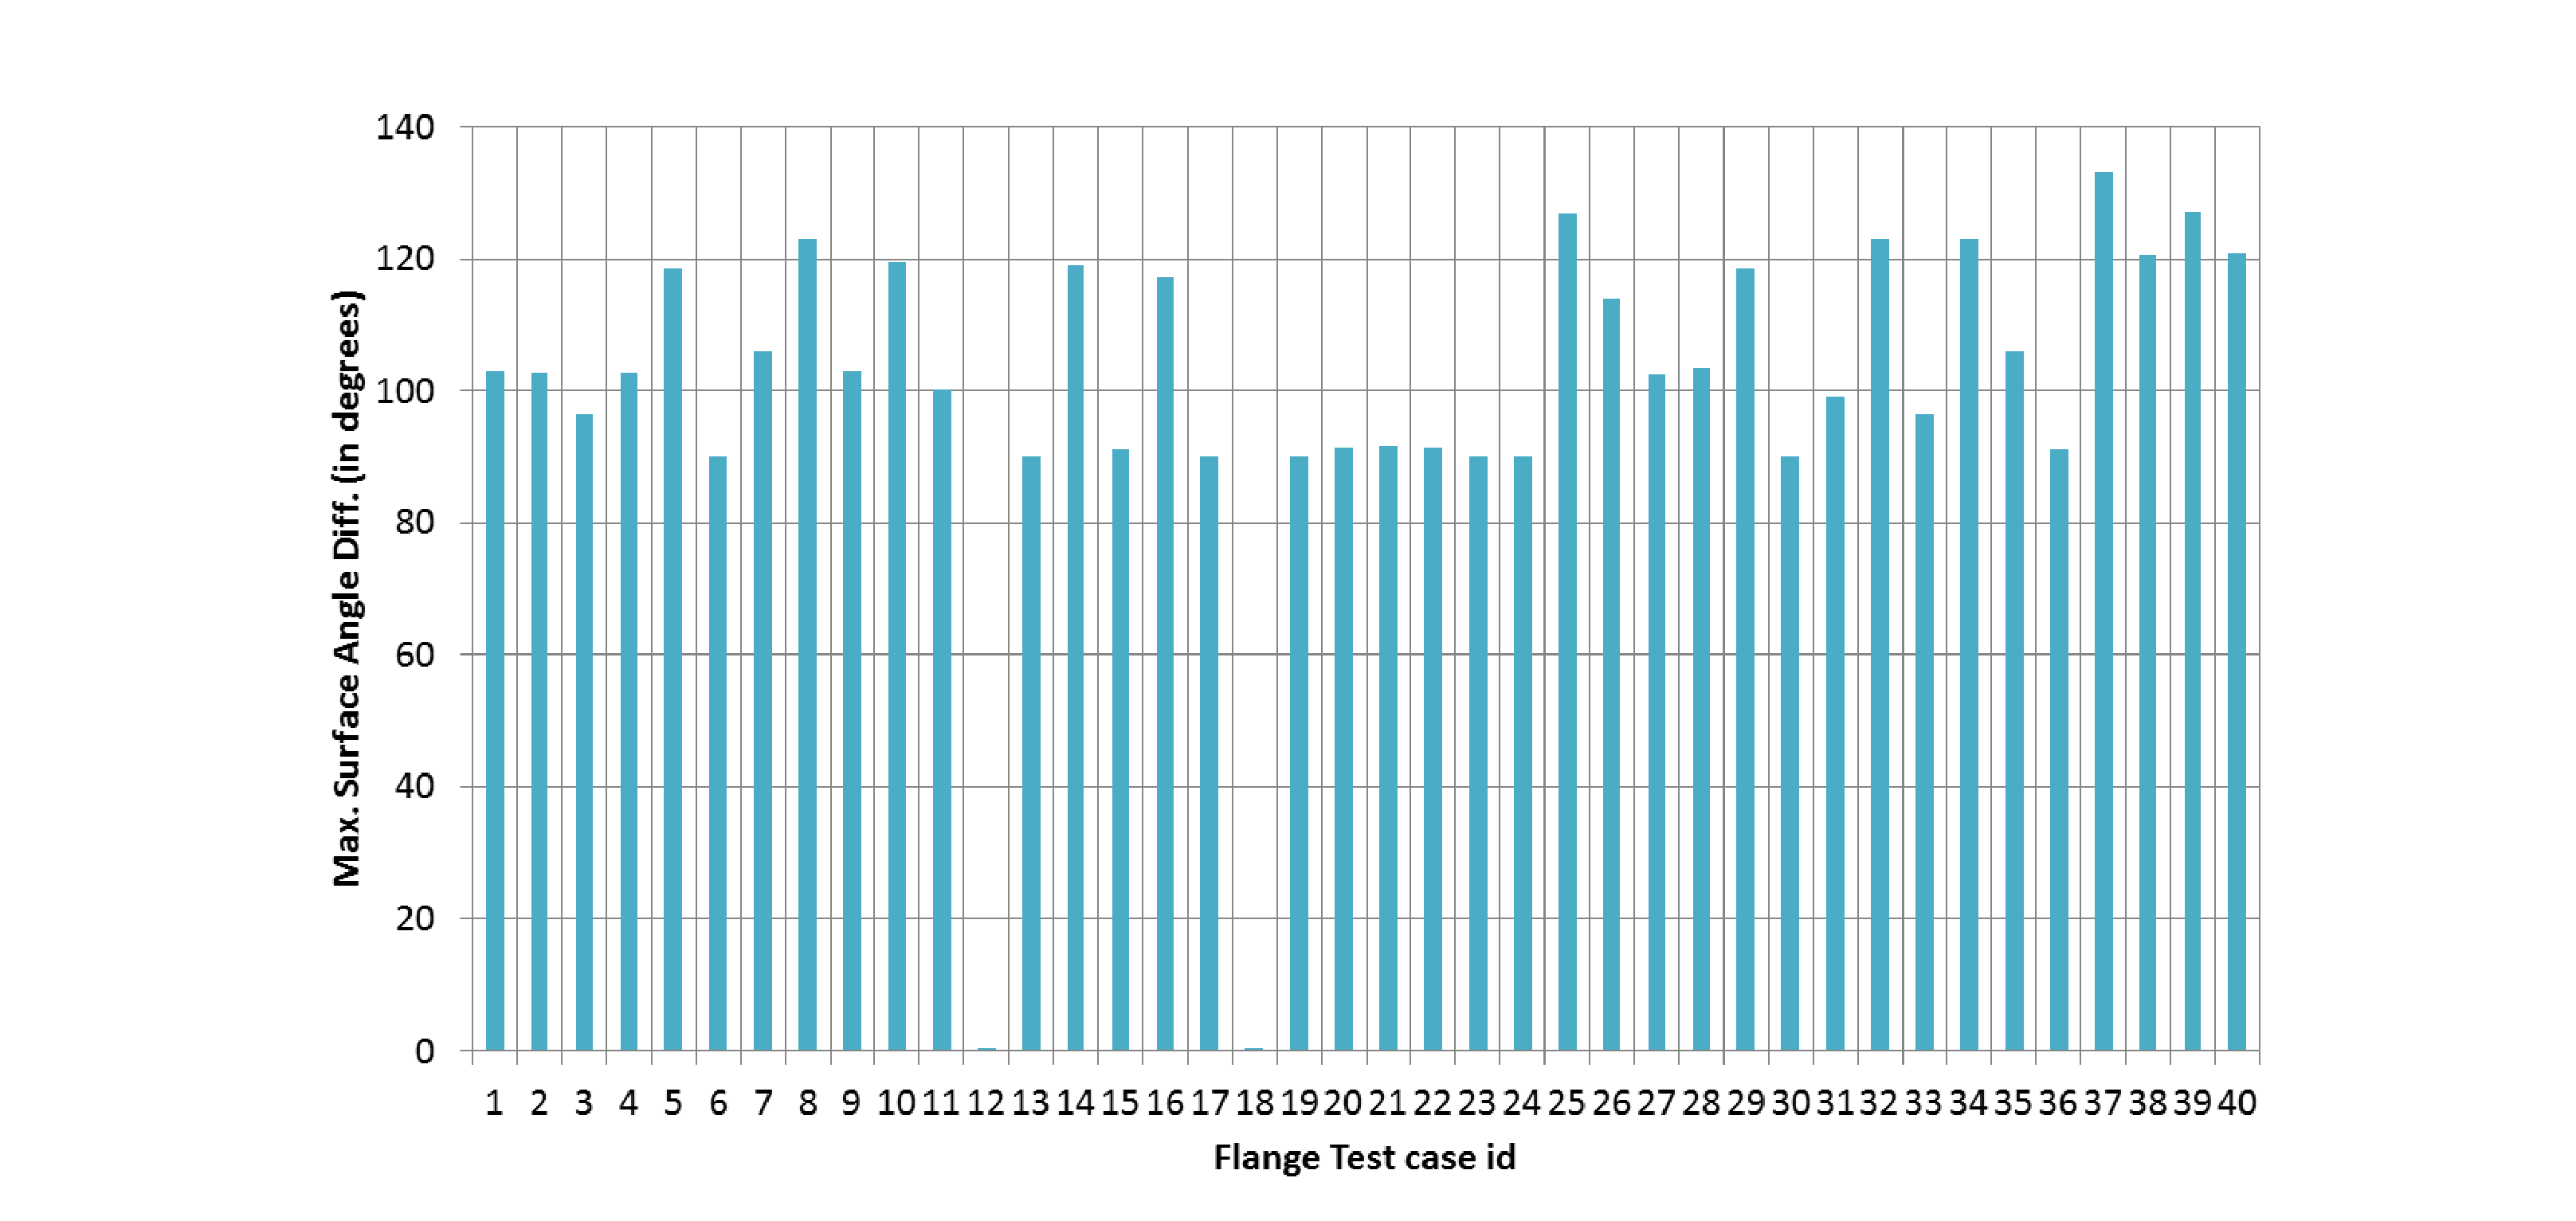
\includegraphics[trim={5cm 0 5cm 0},clip, width=0.45\linewidth]{images/max_surface_angle_Flange.eps}\label{fig:polymender:d}}\\
			\subfloat[]{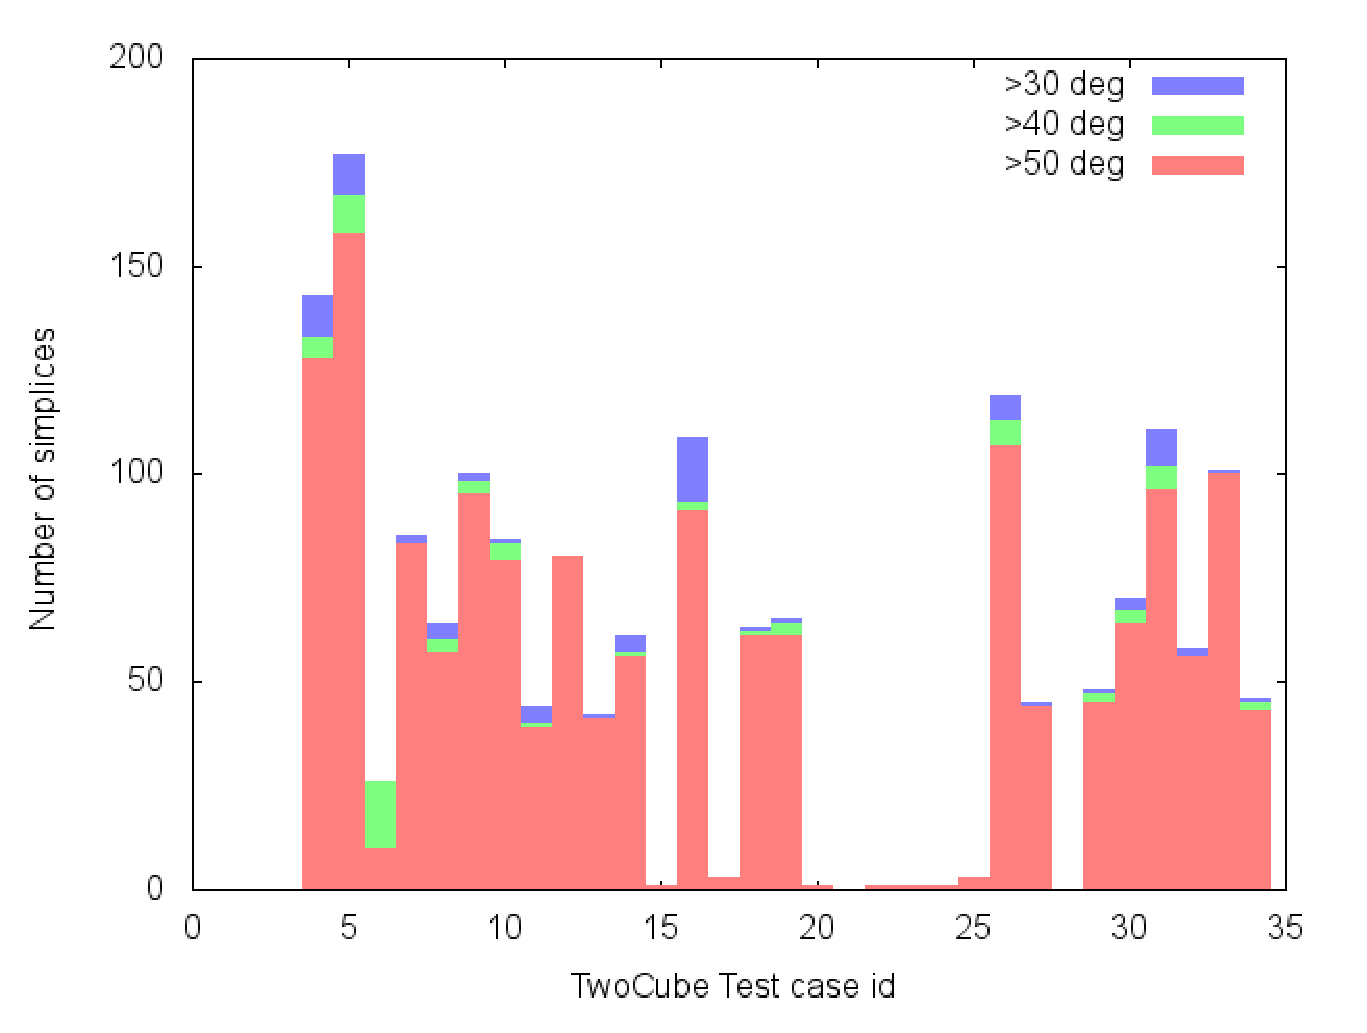
\includegraphics[ width=0.49\linewidth]{images/twocube-35-polymender.eps}\label{fig:polymender:f}}\quad
		\subfloat[]{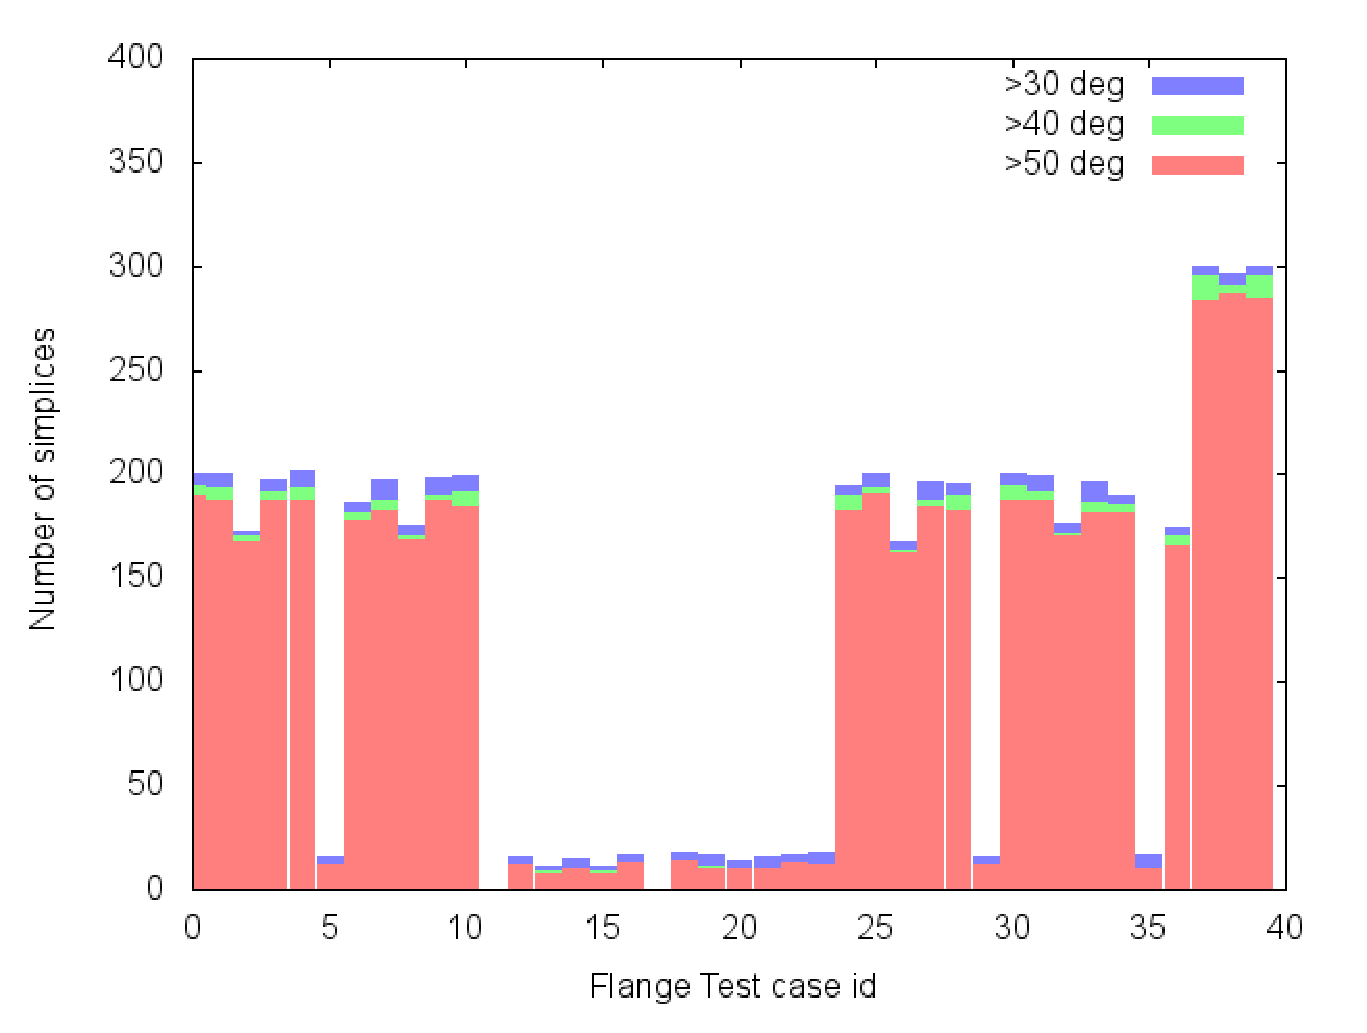
\includegraphics[ width=0.49\linewidth]{images/flange-35-polymender.eps}\label{fig:polymender:e}}\\
		%\subfloat[]{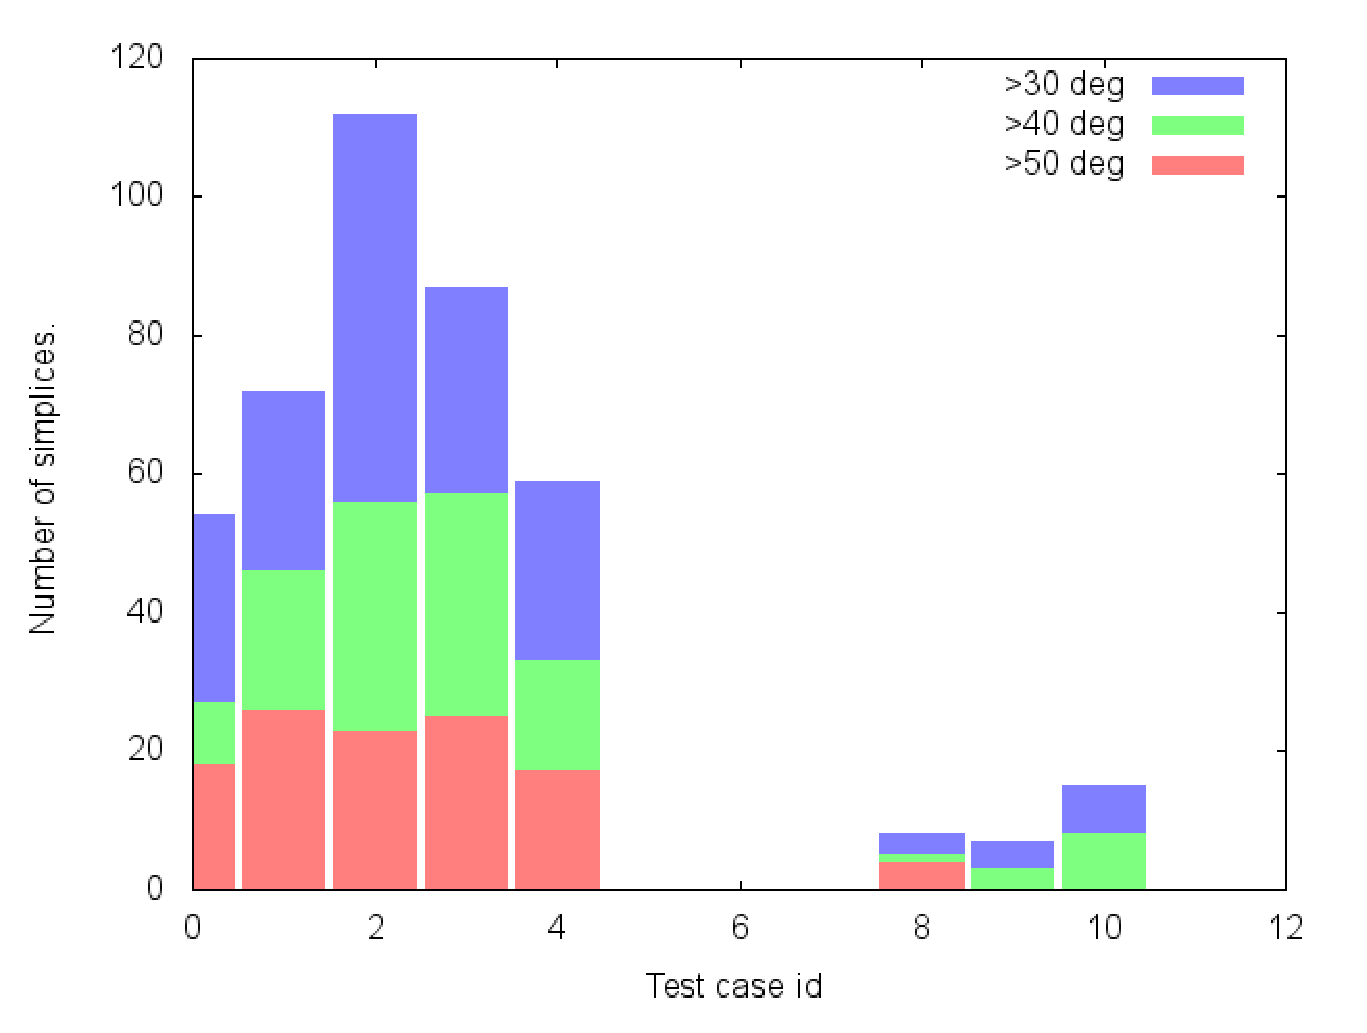
\includegraphics[width=0.3\linewidth]{images/polymender_angle_histogram.eps}\label{fig:polymender:a}}\quad
		%\subfloat[]{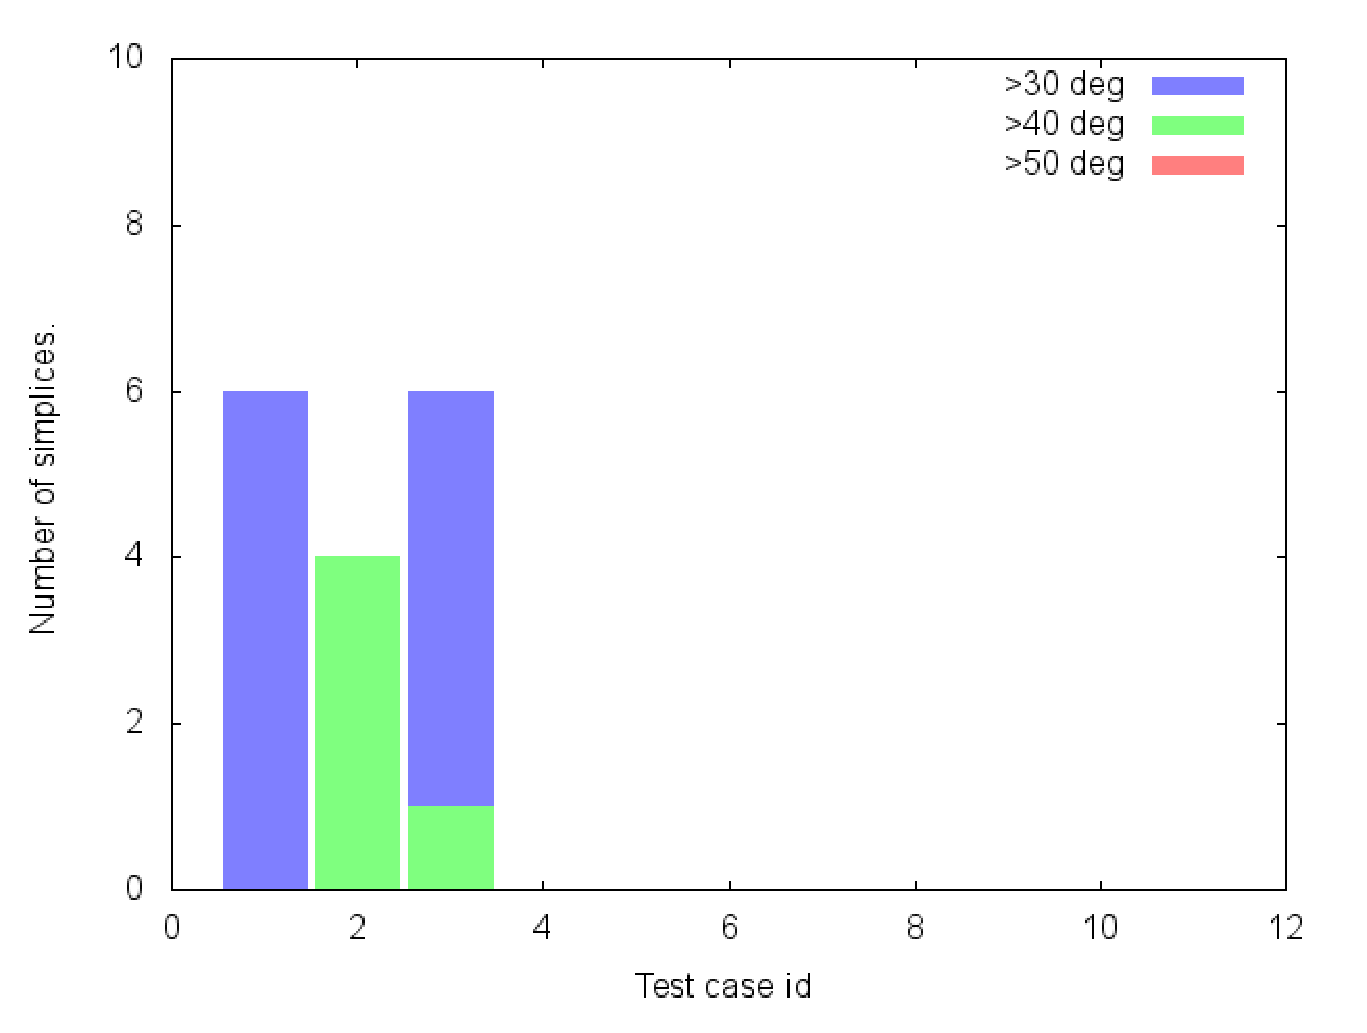
\includegraphics[width=0.3\linewidth]{images/polymender_shrec_compare_1.eps}\label{fig:polymender:b}}\quad		
		\caption{Summary results of Polymender.~\protect\subref{fig:polymender:a} Maximum surface angle difference between Polymender results and perfect mesh for 34 twoCube datasets. 
			~\protect\subref{fig:polymender:b} CountDegree errors for the same dataset.
			~\protect\subref{fig:polymender:c} Maximum surface angle difference between Polymender results and perfect mesh for 40 Flange data sets.
			~\protect\subref{fig:polymender:d} CountDegree errrors for the same datasets. 
			~\protect\subref{fig:polymender:f} Number of simplices with angle difference above 30, 40, 50$^\circ$ for the twoCube datasets.
			~\protect\subref{fig:polymender:e} Number of simplices with angle difference above 30, 40, 50$^\circ$ for the Flange datasets.}	
		\label{fig:polymenderA}
\end{figure*}
\begin{figure*}
	\centering
			\subfloat[]{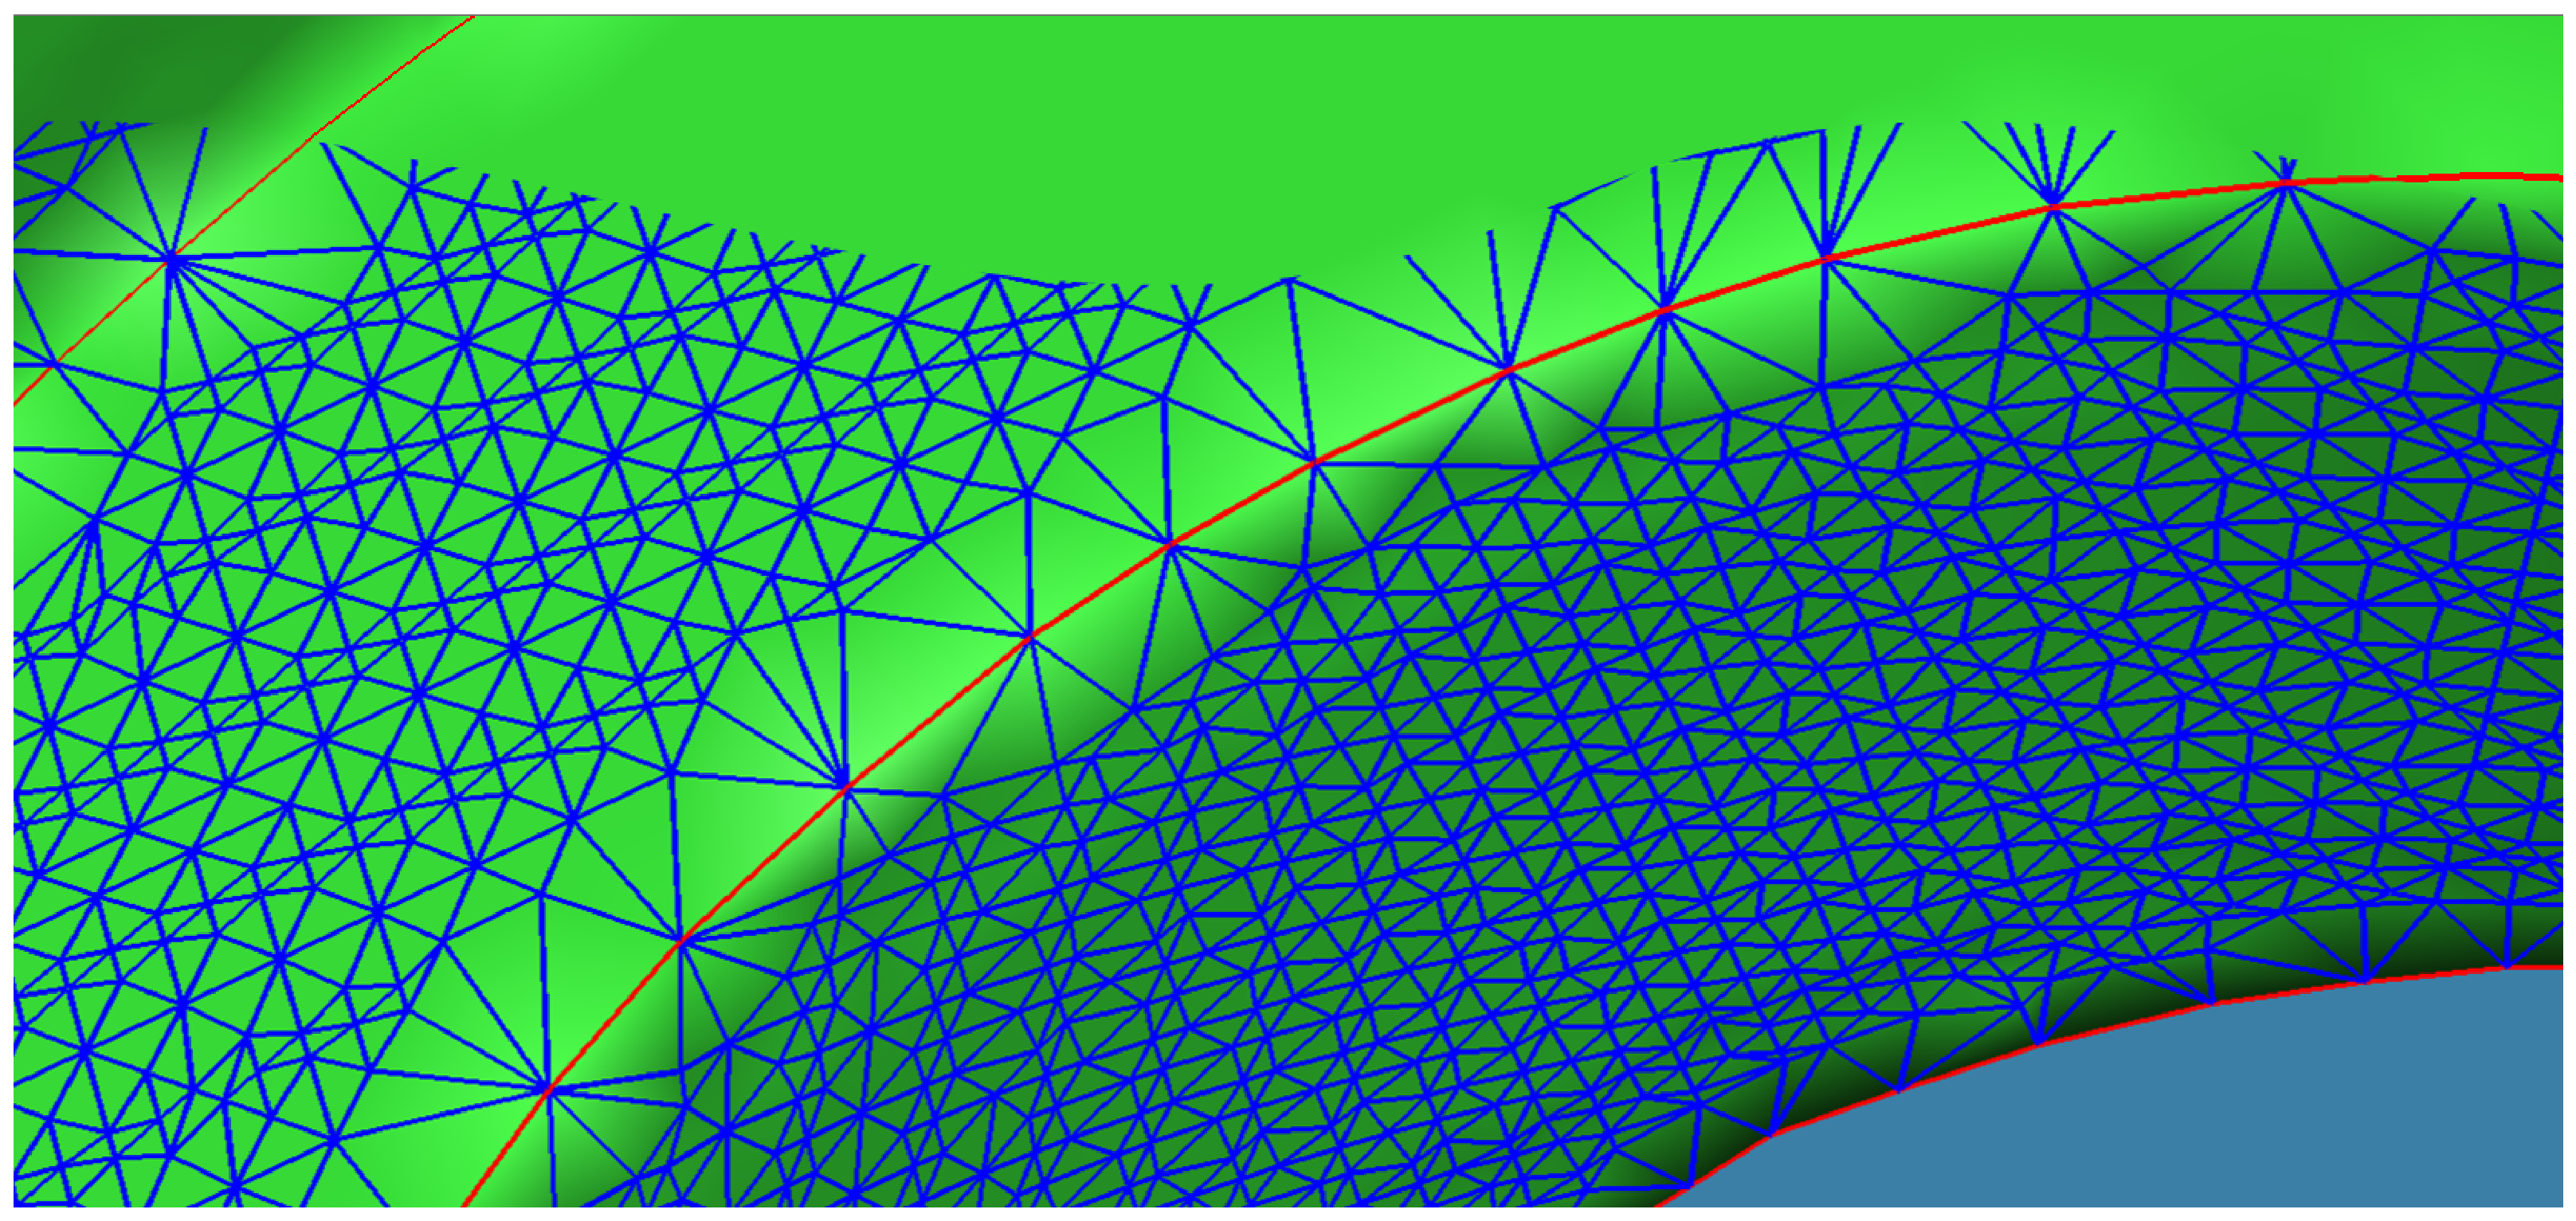
\includegraphics[width=0.33\linewidth]{images/polymender3.eps}\label{fig:polymenderB:a}}\quad
			\subfloat[]{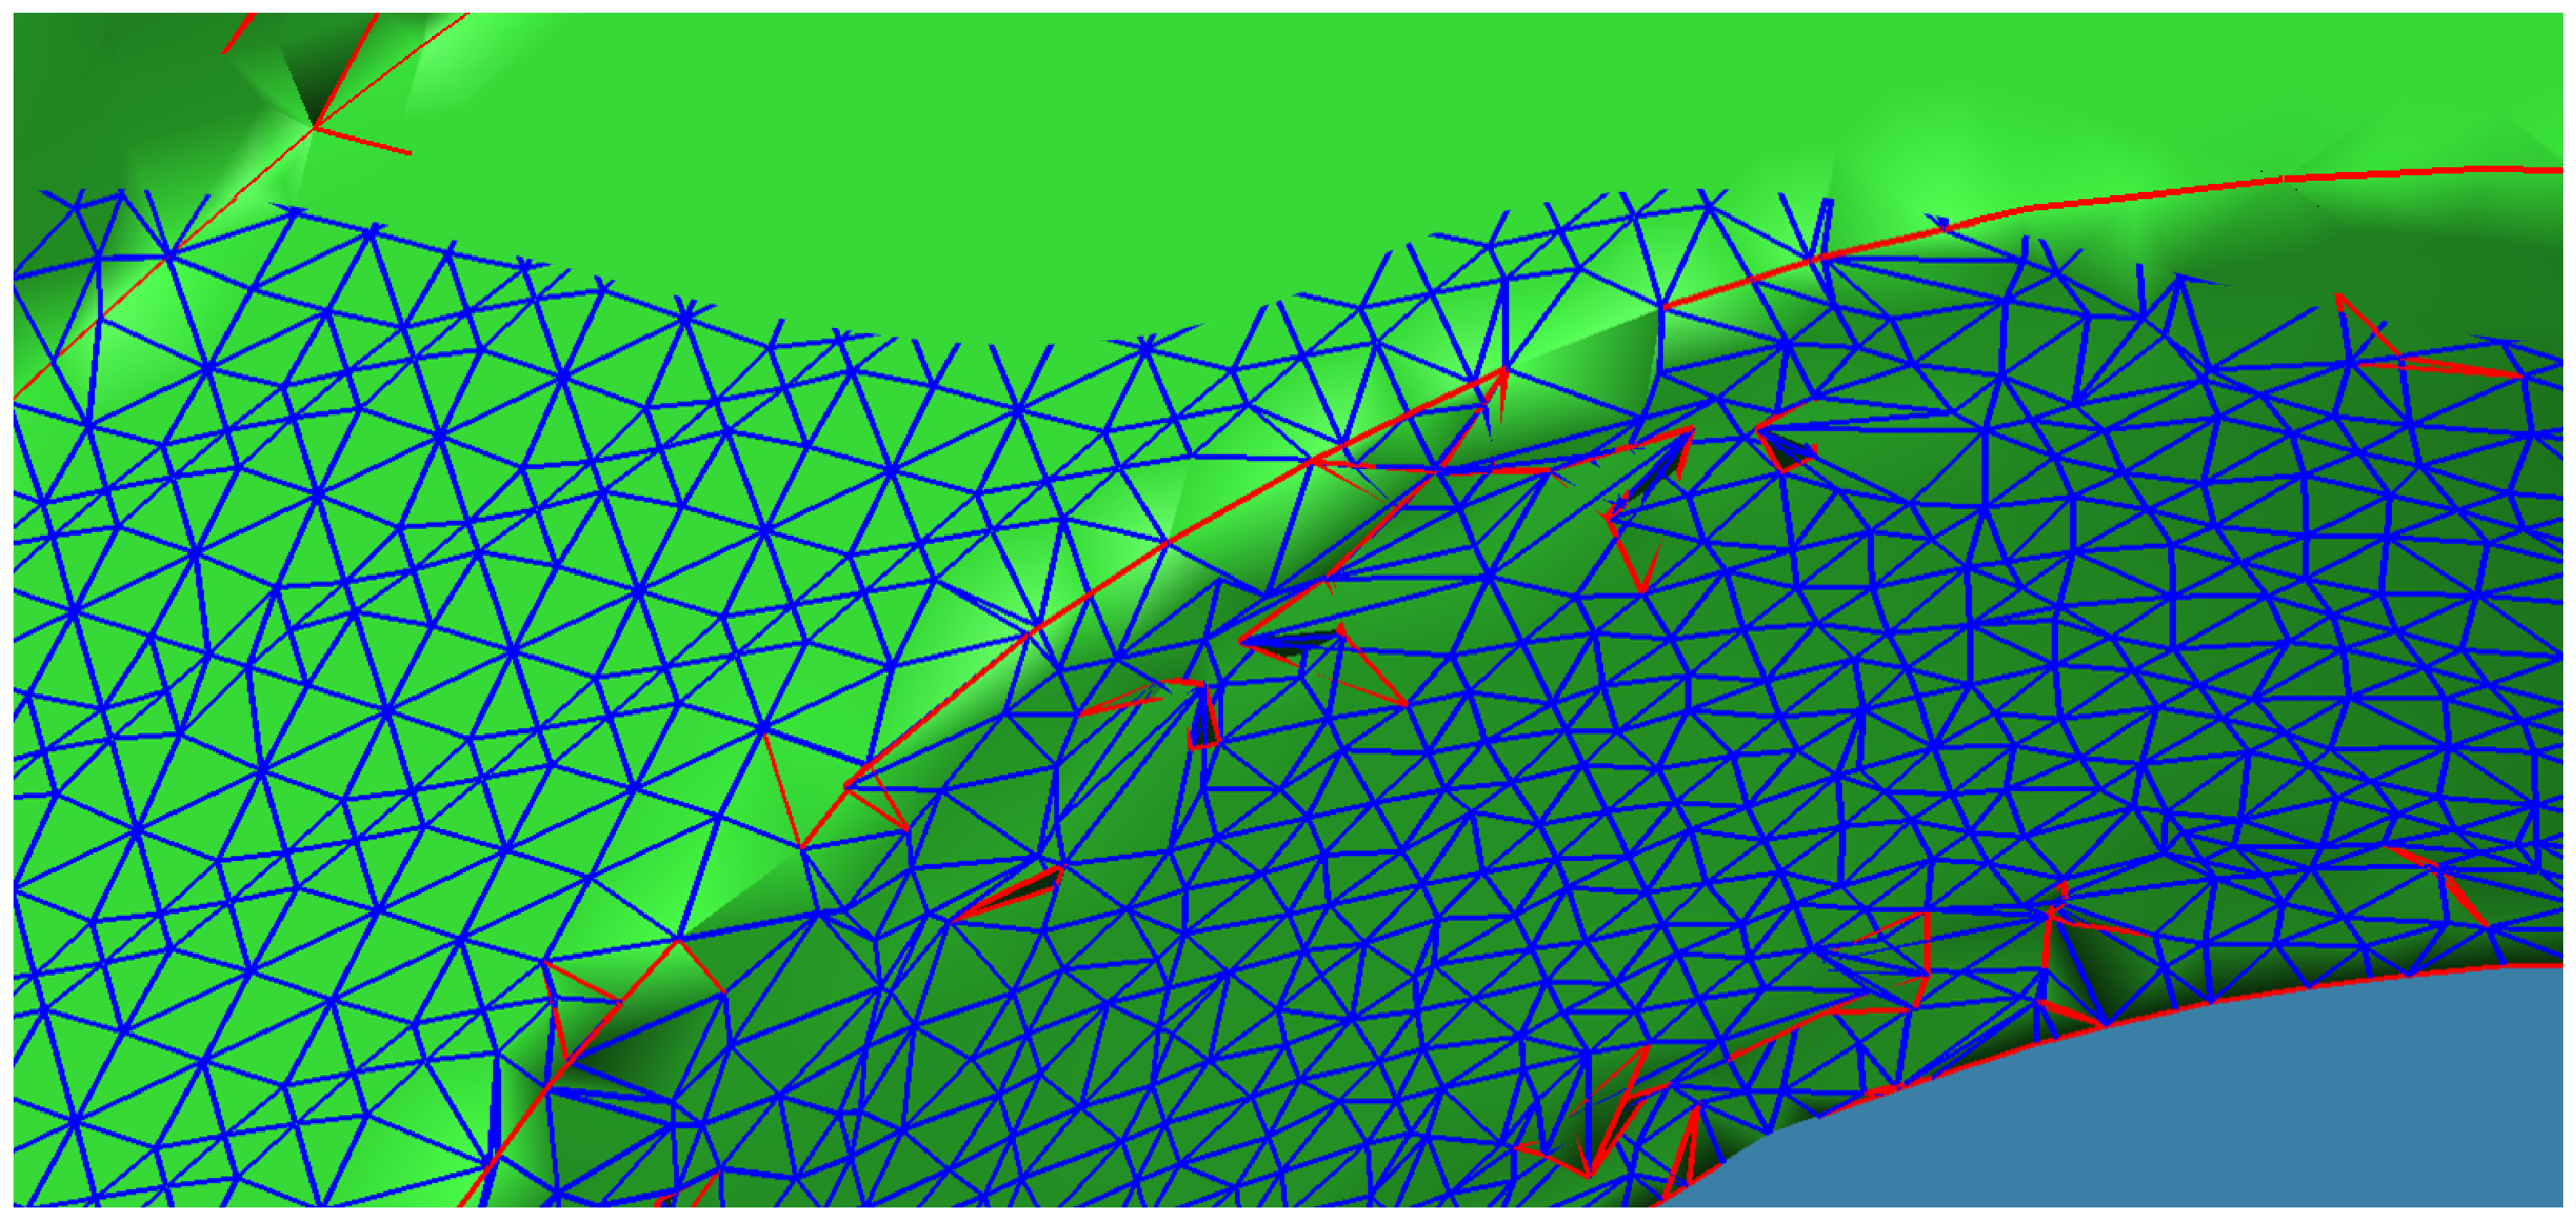
\includegraphics[width=0.33\linewidth]{images/polymender4.eps}\label{fig:polymenderB:b}}
			\subfloat[]{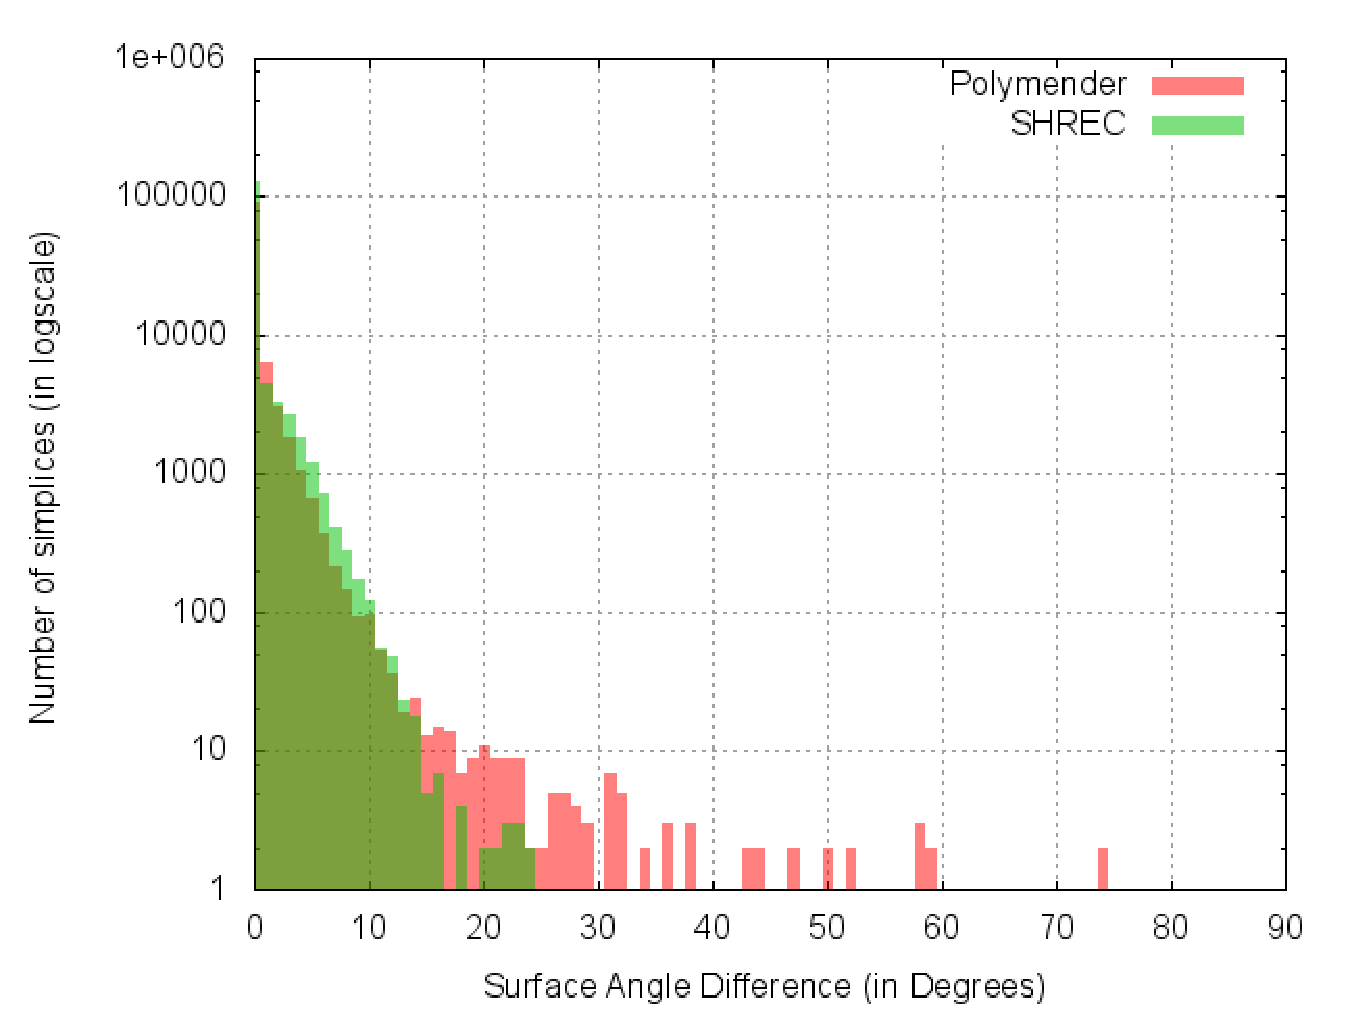
\includegraphics[width=0.3\linewidth]{images/polymenderHistogram_1.eps}\label{fig:polymenderB:c}}\\
			\subfloat[]{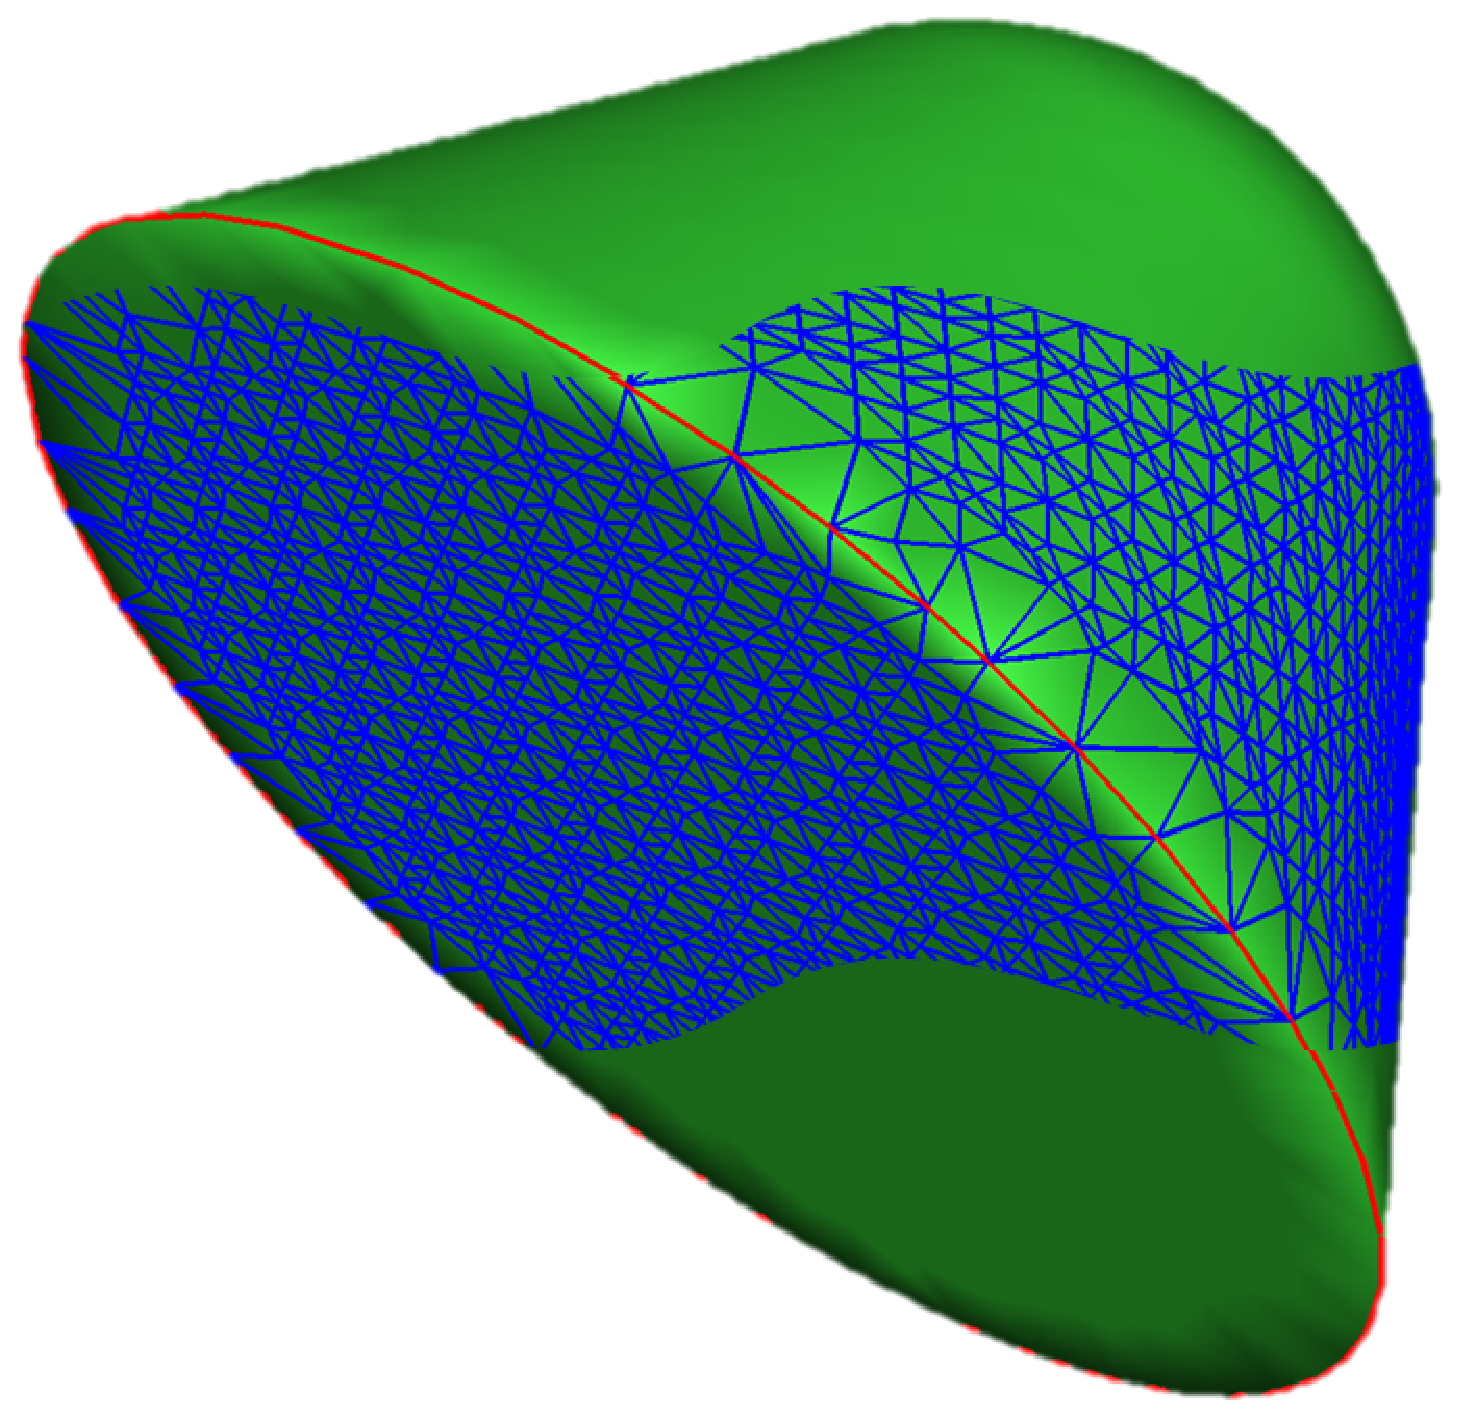
\includegraphics[width=0.2\linewidth]{images/polymender_cone_merge_1.eps}\label{fig:polymender:cone:a}}\quad
			\subfloat[]{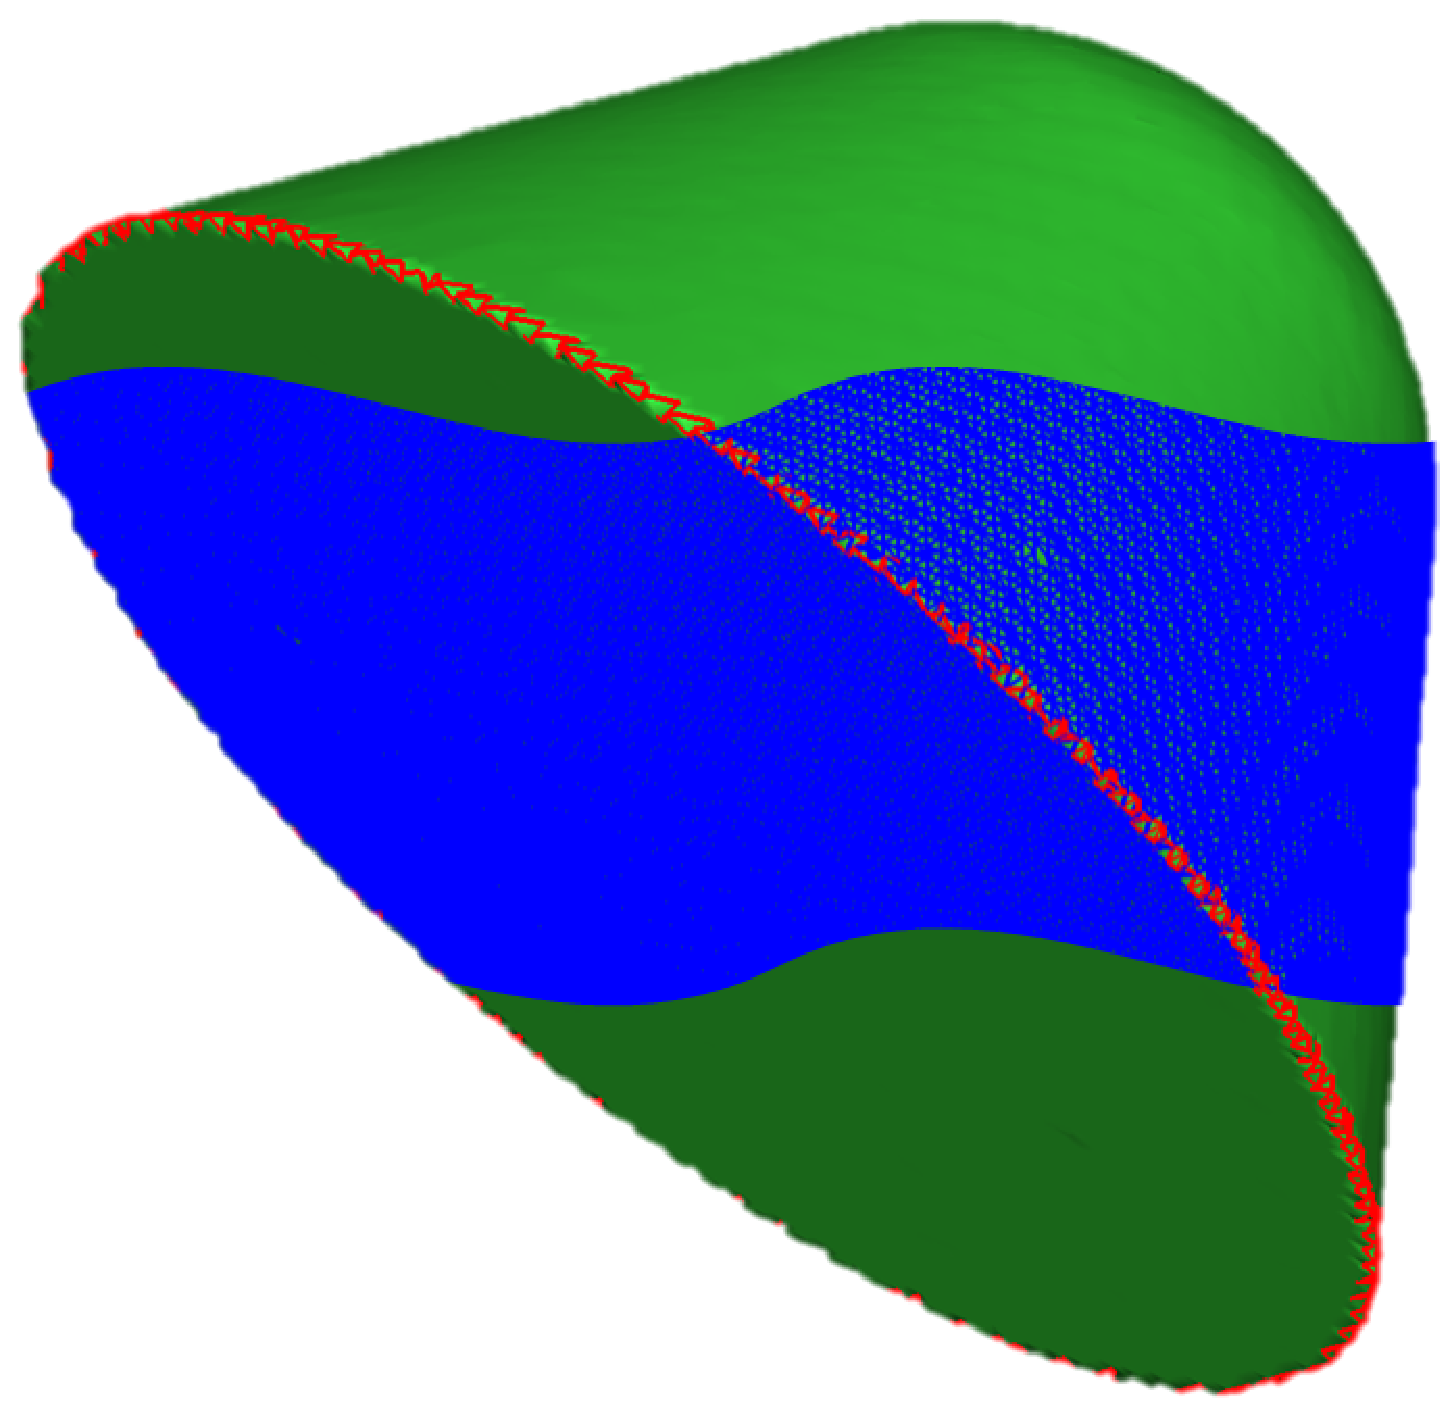
\includegraphics[width=0.2\linewidth]{images/polymender_cone_merge_2.eps}\label{fig:polymender:cone:b}}\quad
			\subfloat[]{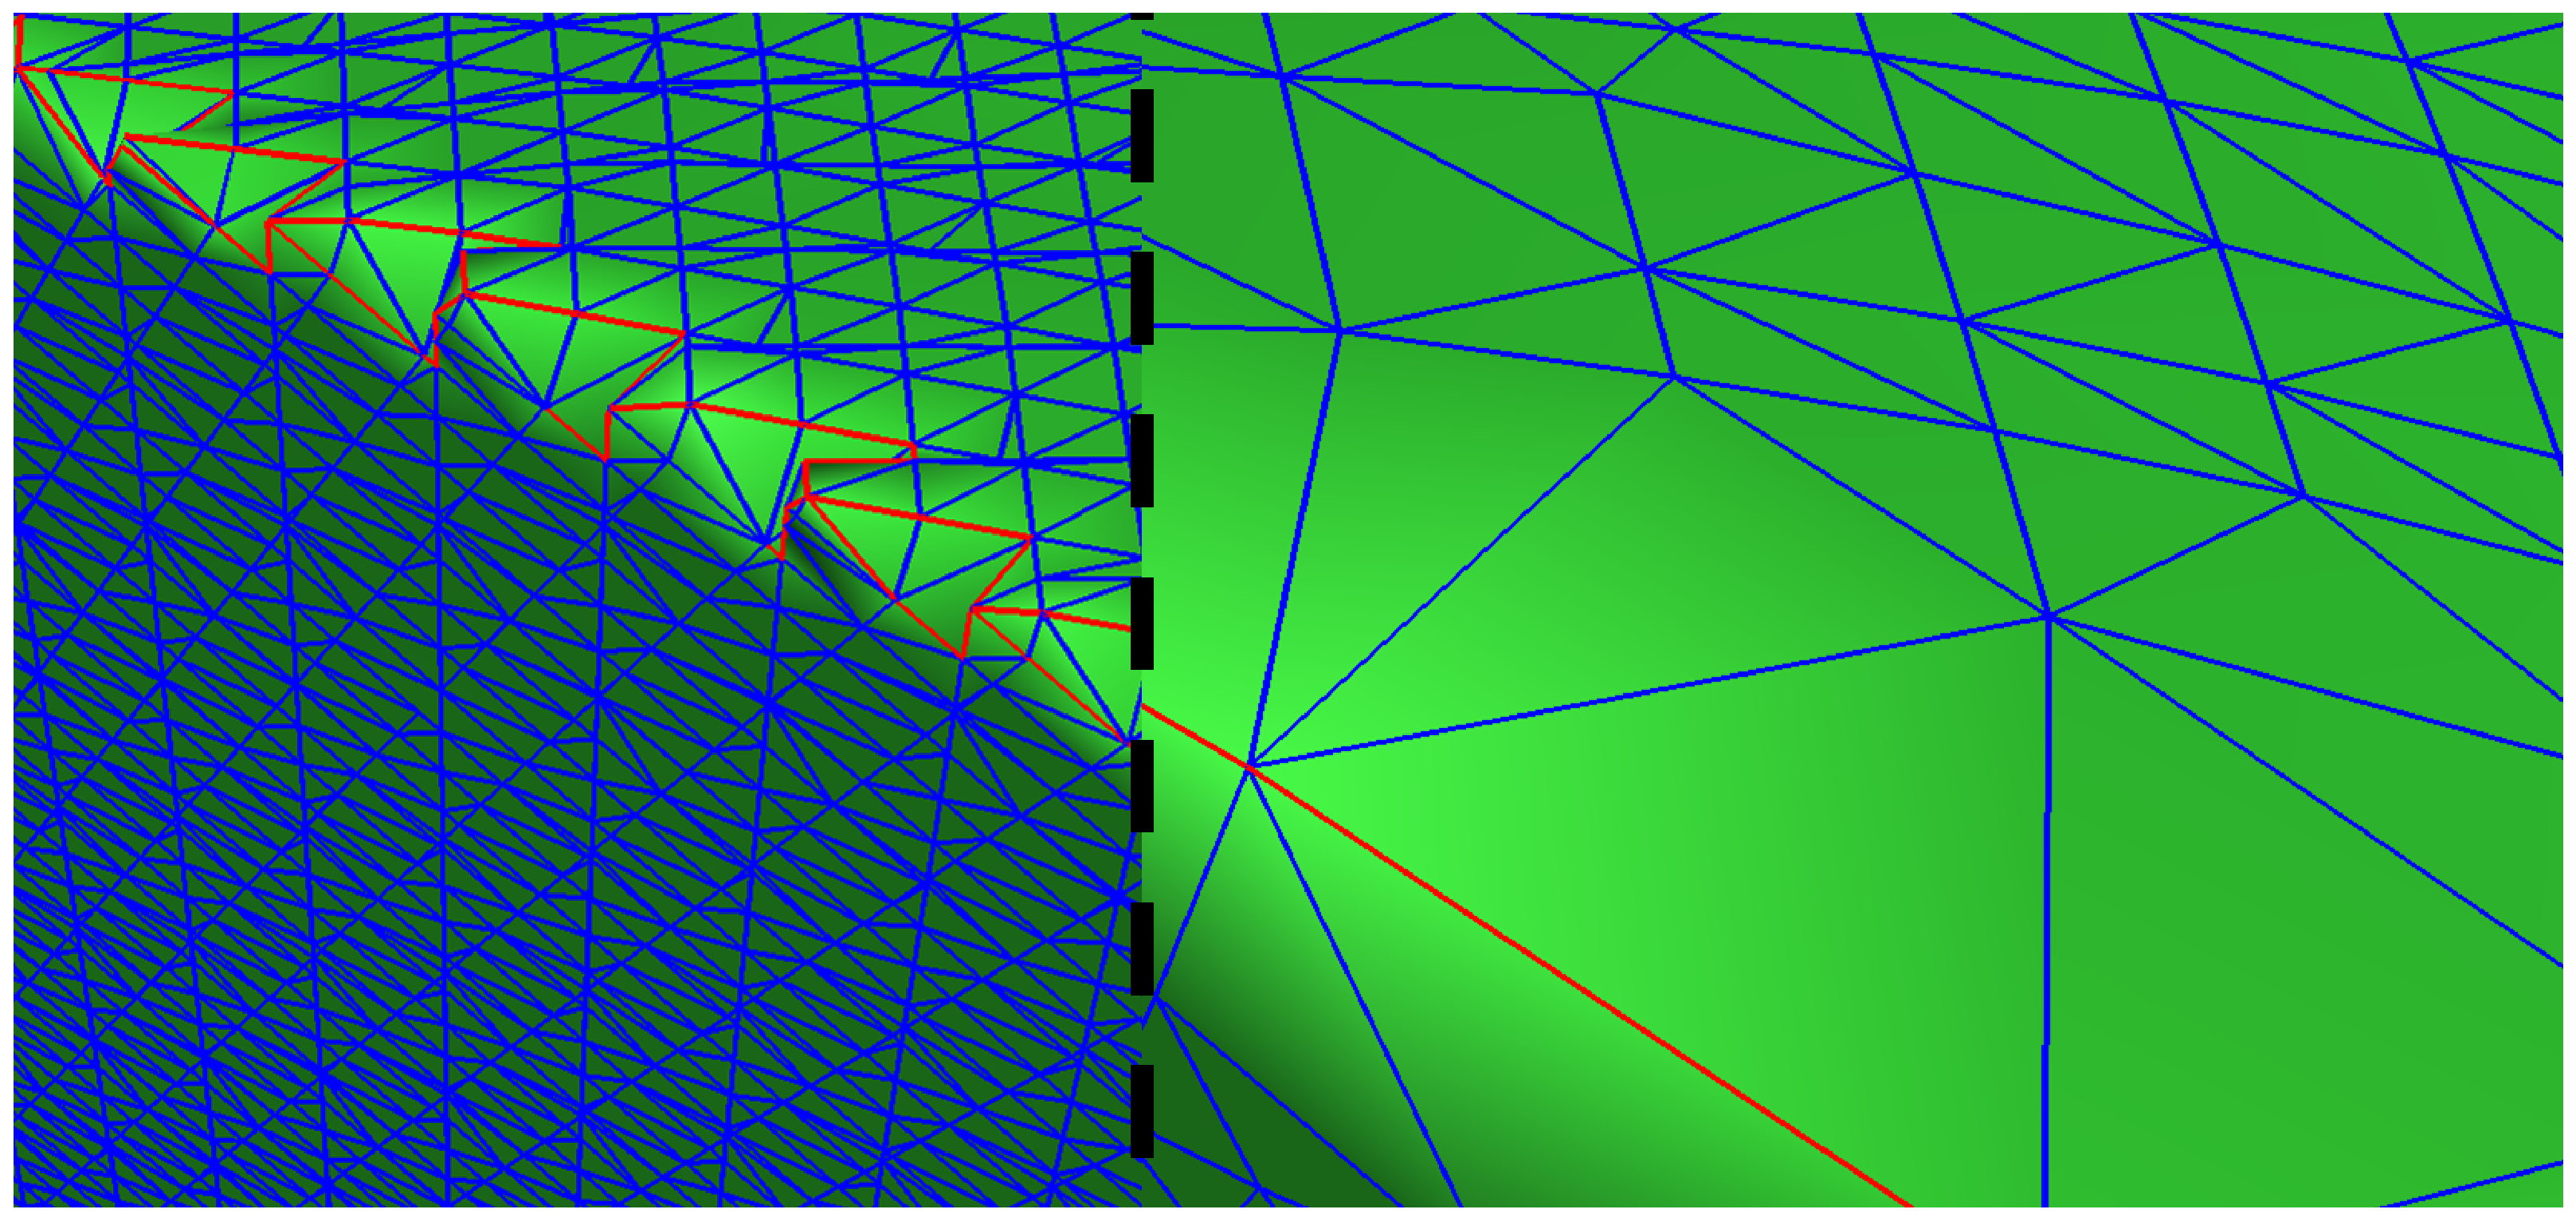
\includegraphics[width=0.4\linewidth]{images/polymender_cone_merge_3.eps}\label{fig:polymender:cone:c}}
			\caption{Shrec vs Polymender. Figure~\protect\subref{fig:polymenderB:a} shows SHREC on a part of the flange dataset. Figure~\protect\subref{fig:polymenderB:b} shows Polymender results. Figure~\protect\subref{fig:polymenderB:c} shows the number of simplices with angle comparison between SHREC and Polymender for this dataset. Figure~\protect\subref{fig:polymender:cone:a} cone dataset using SHREC. Figure~\protect\subref{fig:polymender:cone:b} cone data set using Polymender. Figure~\protect\subref{fig:polymender:cone:c} magnified region showing both. }
					\label{fig:polymenderB}
\end{figure*}
\paragraph{Extended Marching Cubes comparison;}

\begin{figure*}
	\centering
	\subfloat[]{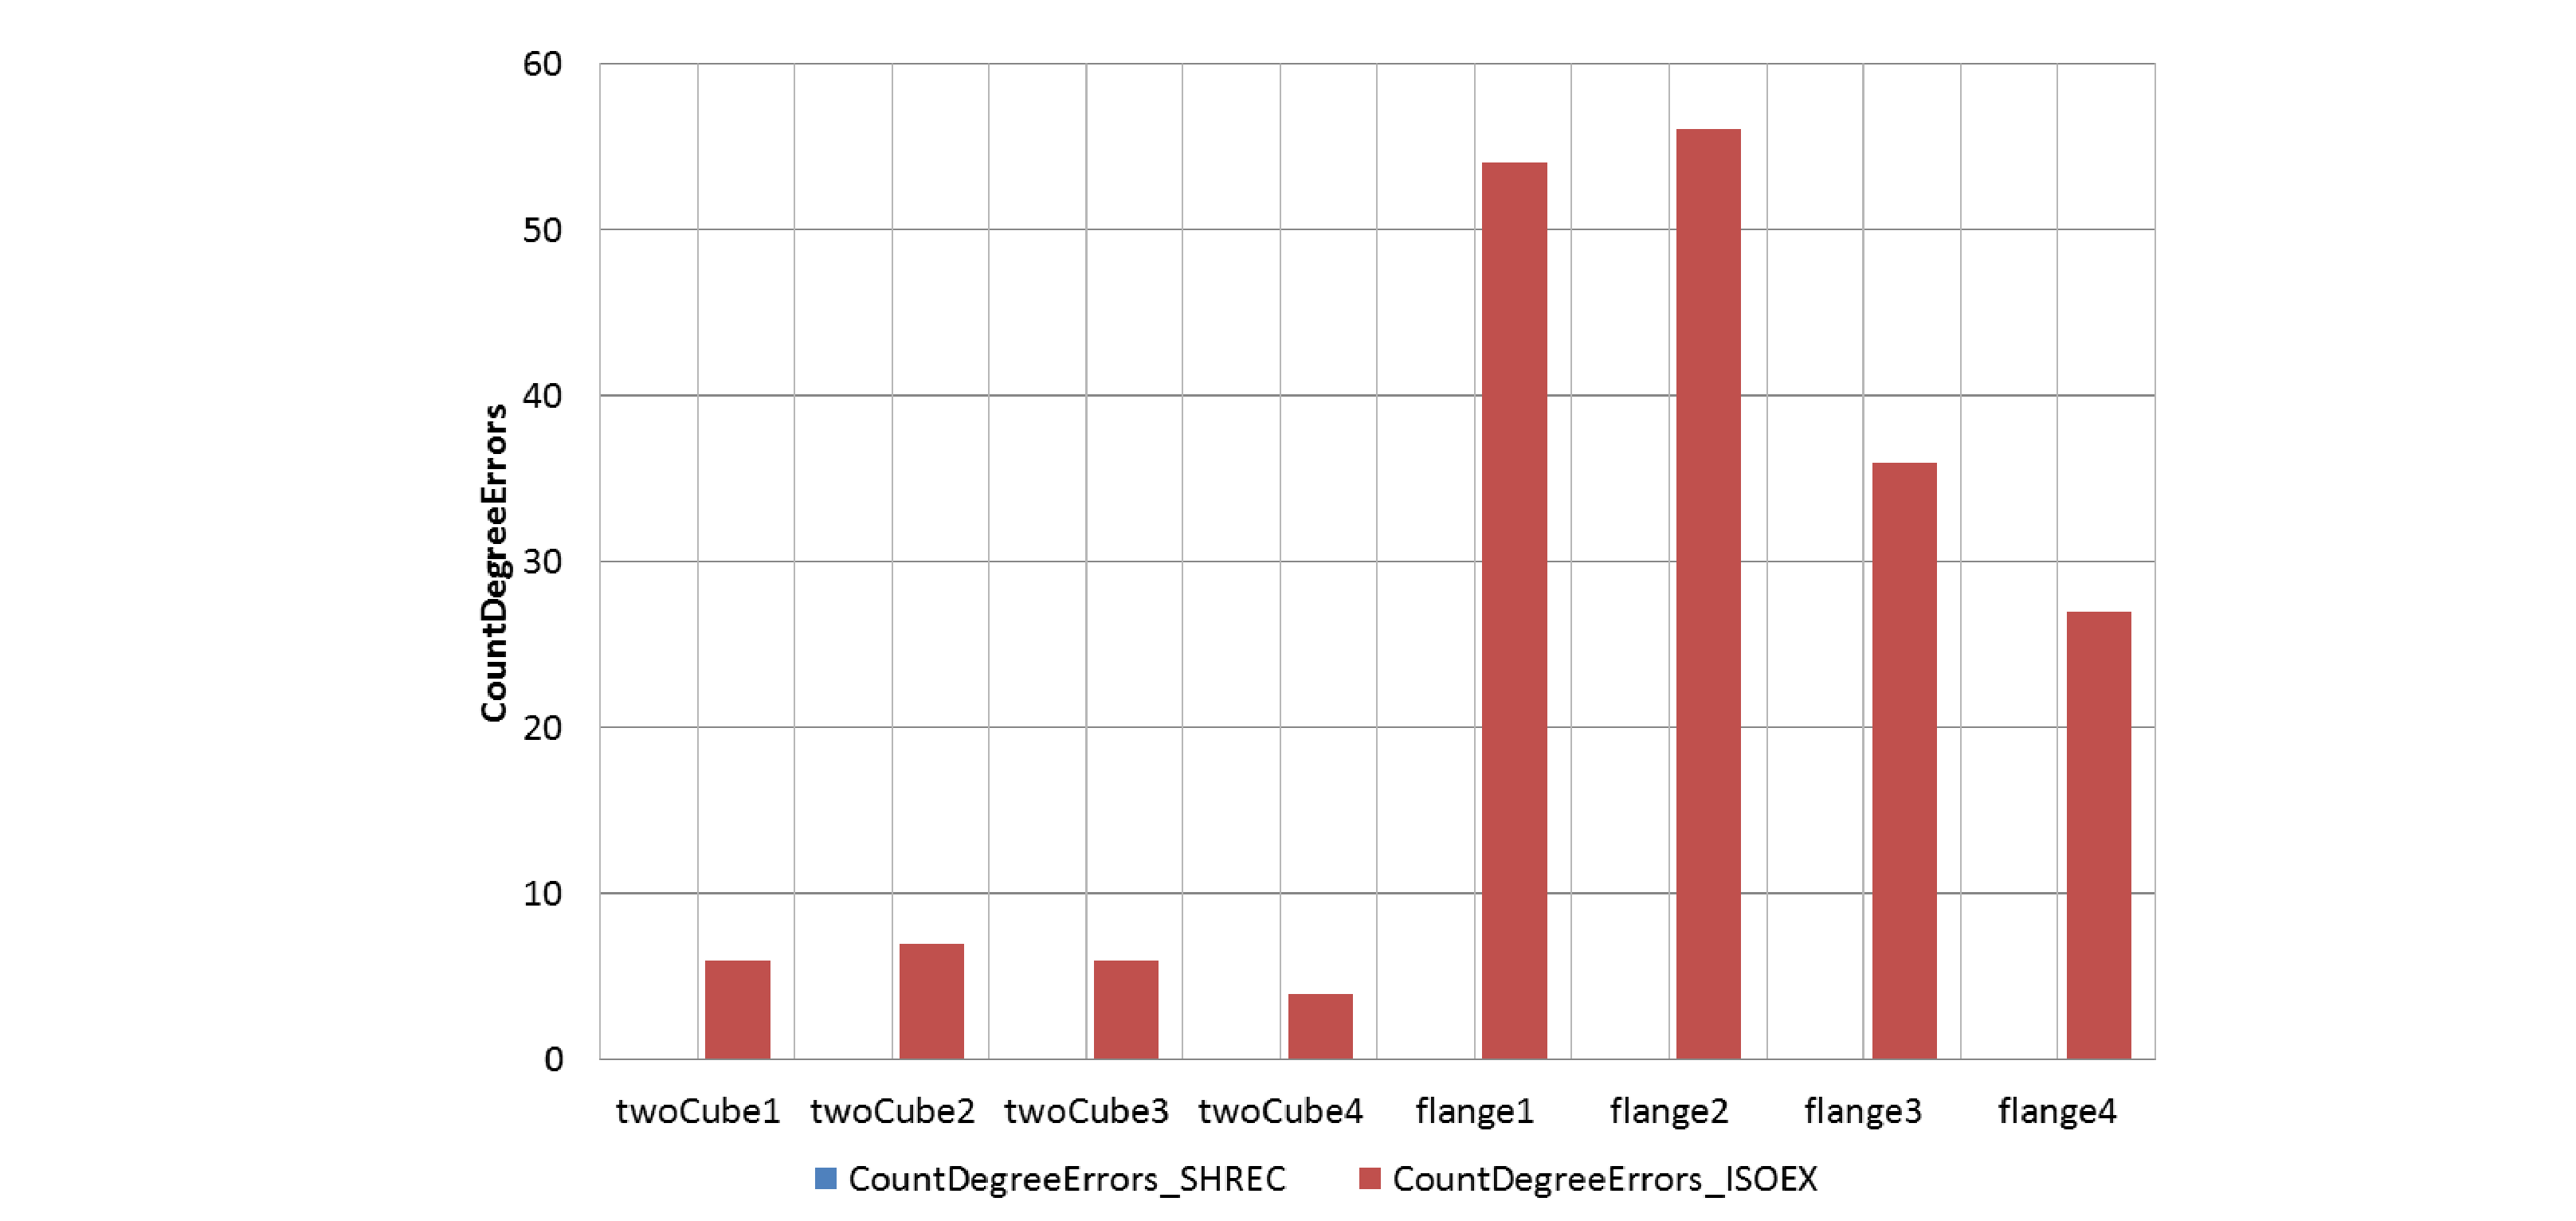
\includegraphics[trim={5cm 0 5cm 0},clip,height=0.2\linewidth]{images/countDegree_isoex.eps}\label{fig:isoEx_summ:a}}
	\subfloat[]{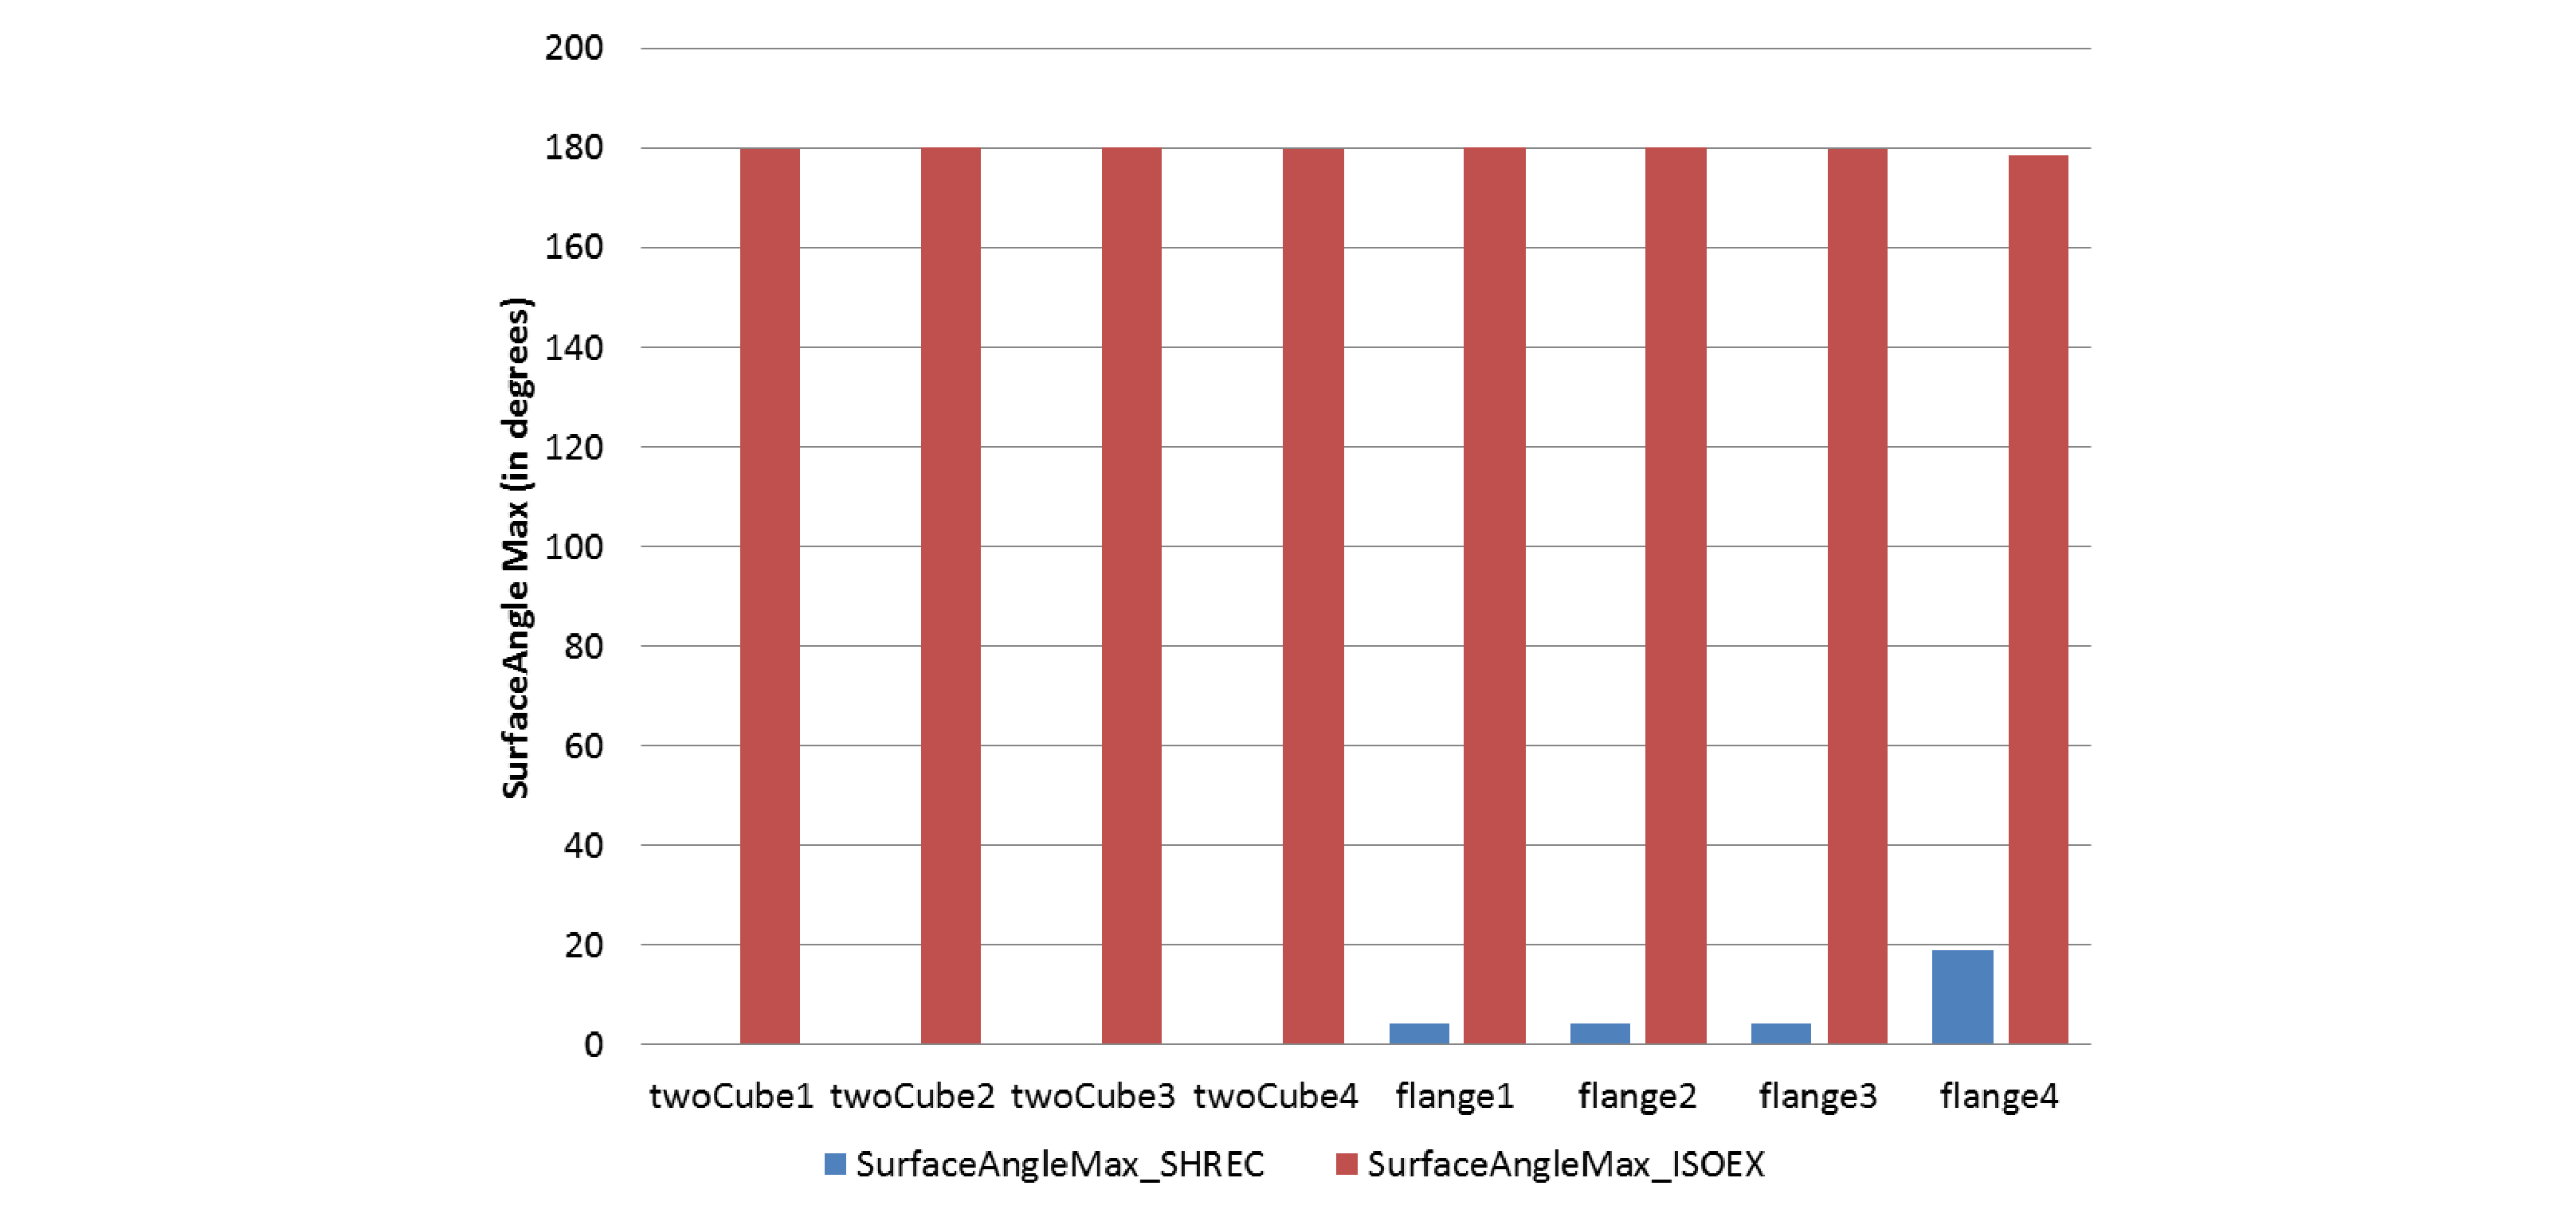
\includegraphics[trim={5cm 0 5cm 0},clip,height=0.2\linewidth]{images/max_angle_isoex.eps}\label{fig:isoEx_summ:b}}
	\subfloat[]{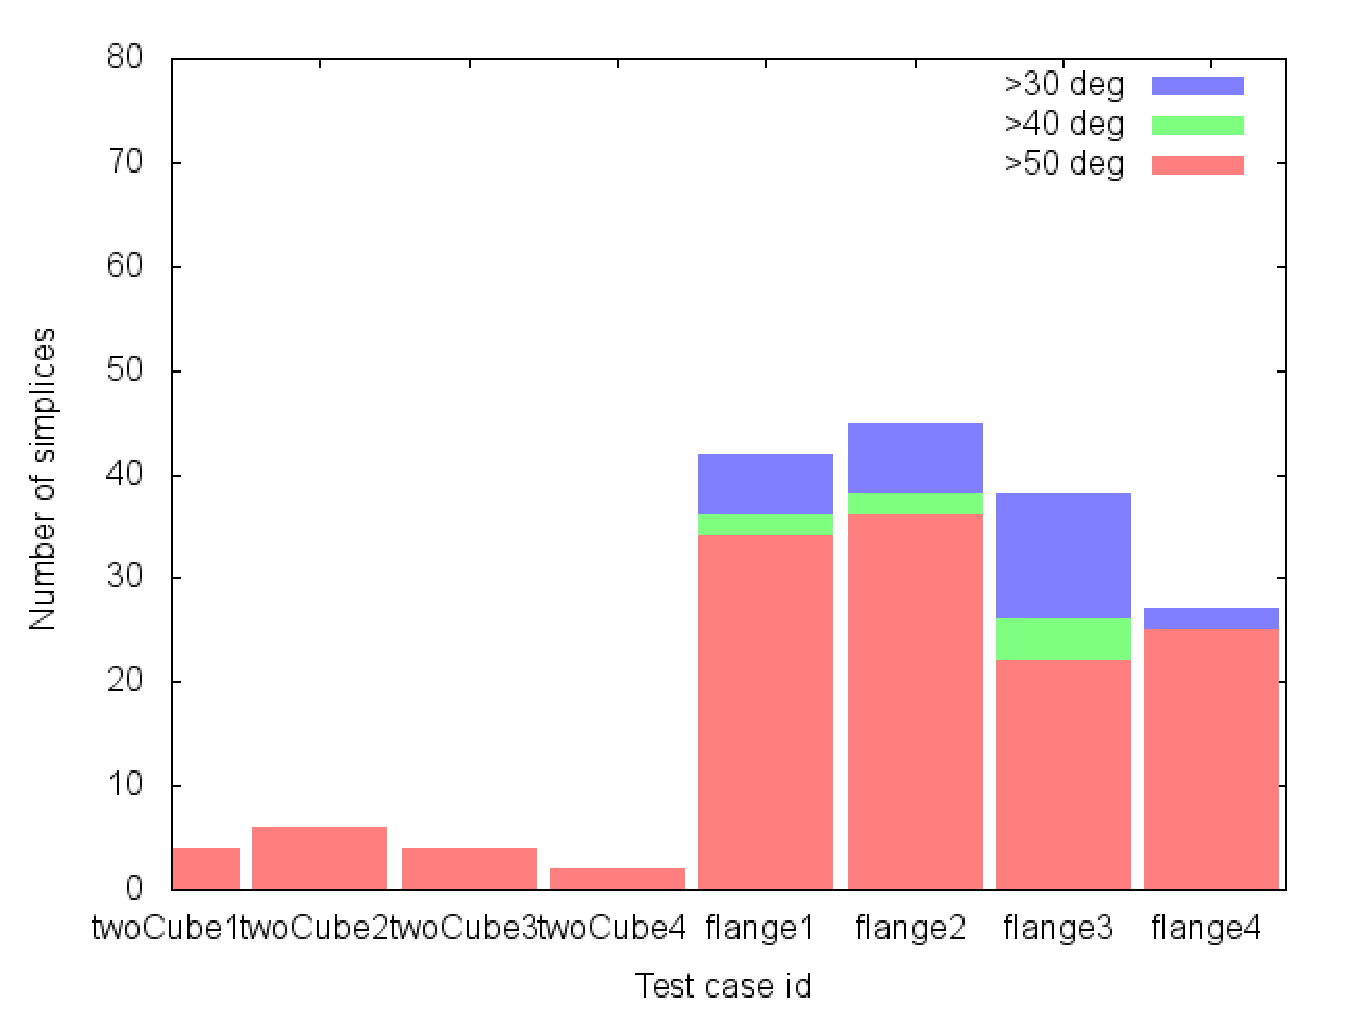
\includegraphics[height=0.2\linewidth]{images/isoex_surf_angle_dist.eps}\label{fig:isoEx_summ:c}}\\
	\subfloat[]{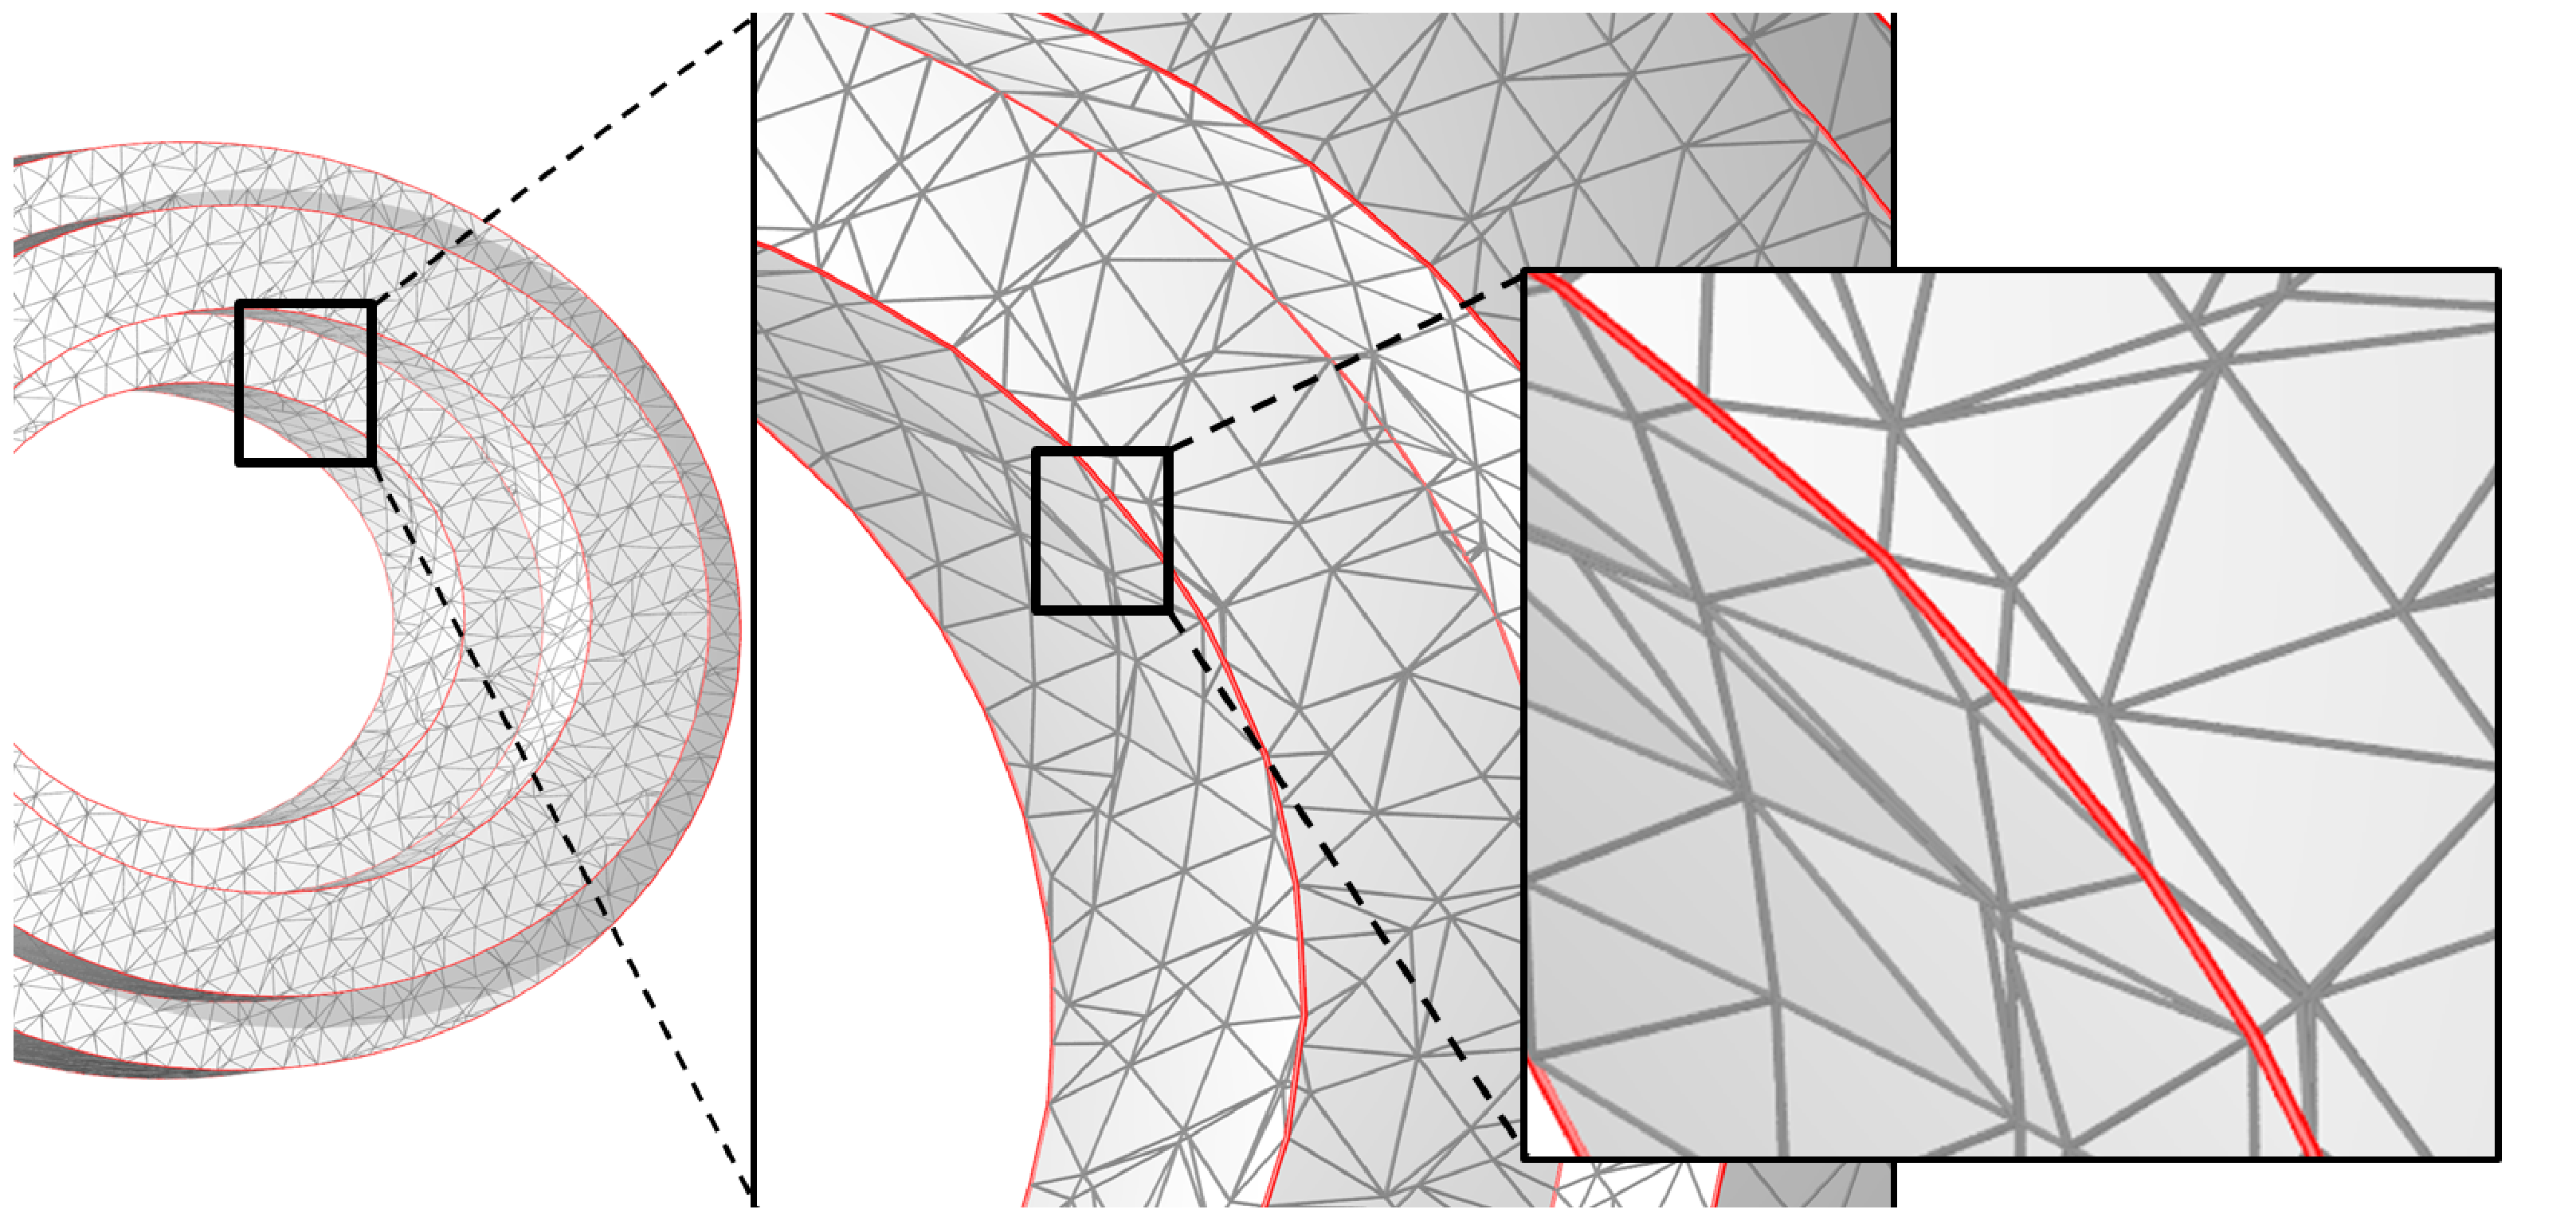
\includegraphics[width=0.5\linewidth]{images/isoExFlange.eps}\label{fig:isoEx:a}}
	\subfloat[]{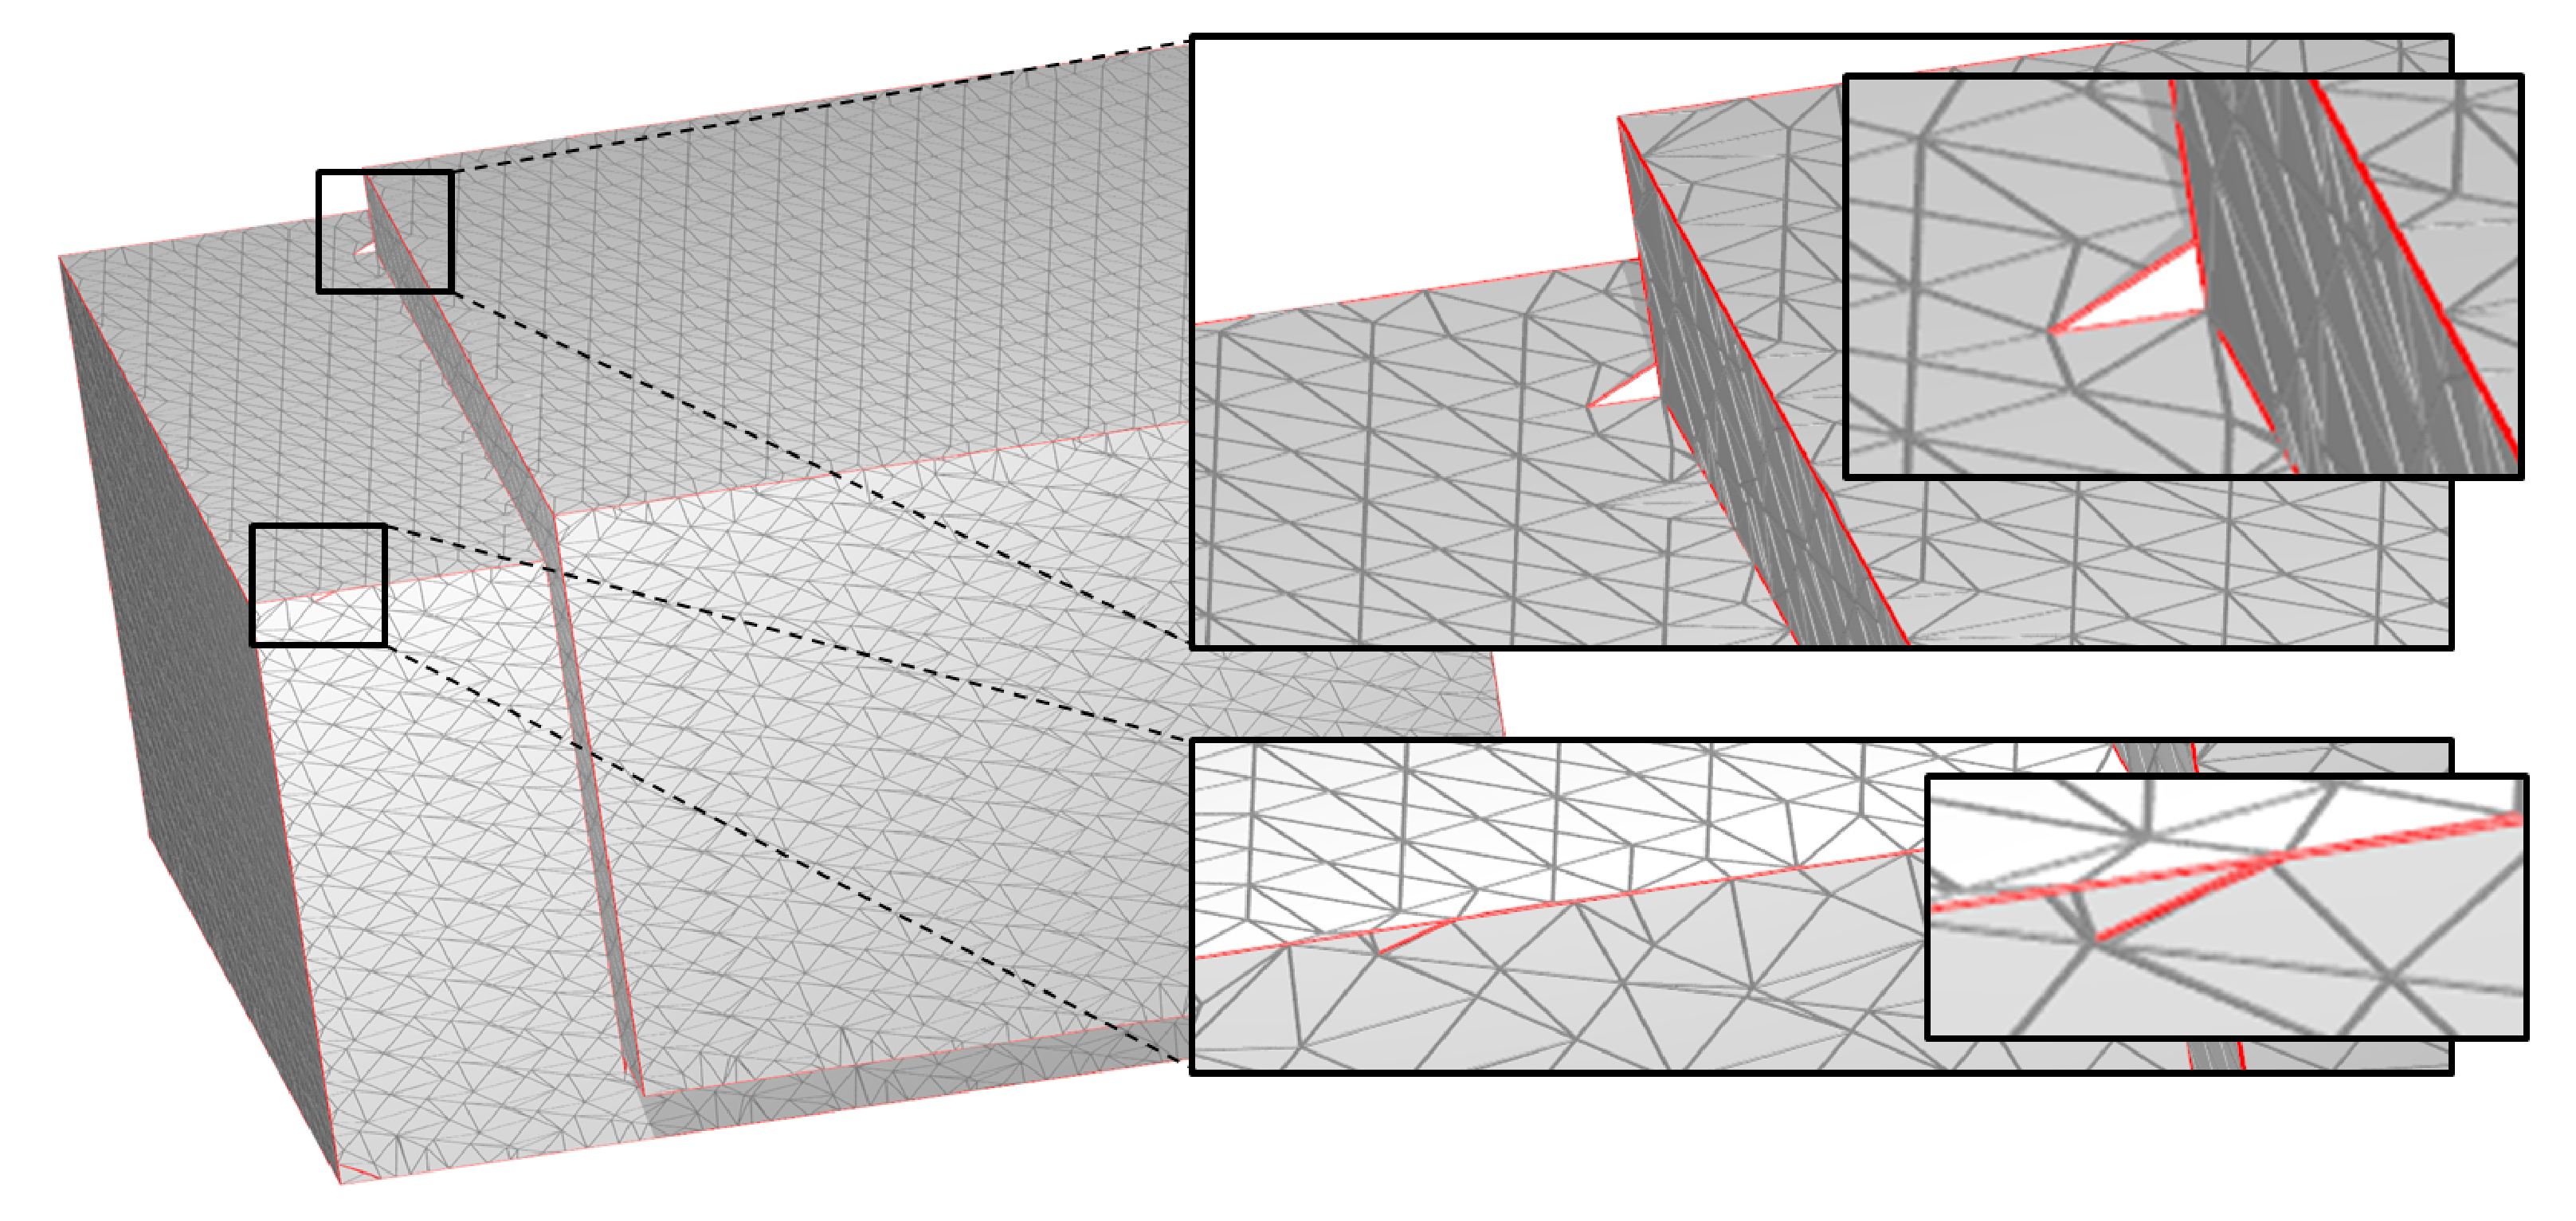
\includegraphics[width=0.5\linewidth]{images/isoExTwoCube.eps}\label{fig:isoEx:b}}\\
	%\subfloat[]{\includegraphics[width=0.45\linewidth]{images/isoex_compare1.eps}\label{fig:isoEx:a}}\quad
	%\subfloat[]{\includegraphics[width=0.45\linewidth]{images/isoEx_compare2.eps}\label{fig:isoEx:b}}
	\caption{Extended Marching Cubes results. (a) Extended Marching Cubes on a Flange dataset. (b) Extended Marching Cubes on a TwoCube dataset.}	
\end{figure*}

We also compare our algorithm to Extended Marching Cubes by Kobbelt et al.~\cite{kbsh-fssev-01}. For this we extended the implementation available at \url{https://www.graphics.rwth-aachen.de/software/} \href{https://www.graphics.rwth-aachen.de/software/}{}, to include twoCube and Flange data types. We ran extended marching cubes on 4 randomly selected twoCube dataset and 4 randomly selected flange dataset. Figure~\protect\subref*{fig:isoEx_summ:a} shows the countDegree results on the test cases using both extended marching cubes and SHREC. SHREC generates no countdegree errors in these testcases, in comparison all test cases using extended marching cubes generate countdegree errors, with the flange testcases generating more errors than the twoCube datasets. Example errors for flange and twoCube are shown in Figure~\protect\subref*{fig:isoEx:a} and Figure~\protect\subref*{fig:isoEx:b} respectively. Figure~\protect\subref{fig:isoEx_summ:b} shows the maximum surface angle difference comparison between SHREC and extended marching cubes. The maximum surface angle difference to the synthetic mesh is less than 20$^\circ$ when using SHREC, but is around 180$^\circ$ for extended marching cubes due to triangle flipping. Finally, Figure~\protect\subref*{fig:isoEx_summ:c} shows the angle distribution for extended marching cubes on the 15 datasets, the reconstruction generates numerous simpices which are at angles greater than 50 $^\circ$ from the synthetic mesh. 

Extensive comparison with the state of the art algorithms show that SHREC with both synthetic gradients and gradients computed from RELIGRAD can out-perform these algorithms and reconstruct sharp features effectively. 


\subsection{Timings}

